\documentclass[10pt,a4paper]{article}
% usepackages
\usepackage[utf8]{inputenc}
%\usepackage[latin1]{inputenc}
%\usepackage[english]{babel}
% math
\usepackage{amsmath}
\usepackage{amsthm}
\usepackage{amsfonts}
\usepackage{amssymb}
\usepackage{mathtools}
\usepackage{latexsym}
% formatting
\usepackage{parskip}
\usepackage{fullpage}
\usepackage{pgf,tikz}
\usepackage{mathrsfs}
\usetikzlibrary{arrows}
\usepackage[round]{natbib}
\usepackage{multirow}
%\pagestyle{empty}
% graphics
%\usepackage[pdftex]{graphicx}
\usepackage{caption}
\usepackage{subcaption}
%\usepackage[below,section]{placeins} % the one below is better for short assignments
\usepackage{float} % provides H as float placement specifier
% extras
\usepackage[pdftex,a4paper,colorlinks=true,urlcolor=blue]{hyperref}
\urlstyle{same}
\usepackage{moreverb} %\verbatimtabinput{filename.py} preserves indentation
\graphicspath{ {images/} }
%Numbering first level list roman (i,ii,iii) instead of arabic (1,2,3)
% options are \roman \Roman \alph \Alph \arabic
%\renewcommand{\theenumi}{\roman{enumi}} 
%\renewcommand{\theenumii}{\roman{enumii}}
%\newcommand{\Int}{\int\limits}
\pagenumbering{arabic}
% Also achieved with the enumerate package
\usepackage{enumerate}
%\numberwithin{equation}{section}%

% author/title details
\author{Alice NANYANZI (\href{mailto:alicenanyanzi@aims.ac.za}{alicenanyanzi@aims.ac.za})}
% \title{Course Title: Assignment X}
% Theorems are in italics.
\theoremstyle{plain}
\newtheorem{thm}[subsection]{Theorem}
%
% Rest is not in italics.
\theoremstyle{definition} 
\newtheorem{lem}[subsection]{Lemma}
\newtheorem{cor}[subsection]{Corollary}
\newtheorem{conj}[subsection]{Conjecture}
\newtheorem{prop}[subsection]{Proposition}
\newtheorem{exa}[subsection]{Example}
\newtheorem{defn}[subsection]{Definition}
\newtheorem{rem}[subsection]{Remark}

\title{THESIS DRAFT}
\date{\today}
\begin{document}
	\maketitle
	\section*{Abstract}
	\newpage
	\listoffigures
	
	\listoftables
	\newpage

	
	\section*{Outline of the Thesis}
	\begin{enumerate}
		\item Abstract
		\item Introduction
		\begin{itemize}
			\item Brief intro of networks
			\item Gaps
			\item Say what you are going to do
			\item Why and how are you going to do the above (importance, how it addresses the Gaps) 
			\item Context - compare to others
			\item Structure of the thesis
		\end{itemize}
	    \item Chapter 1: Review of networks
	     \begin{itemize}
	     	\item Similarity in networks
	     	\item Voronoi Tesselation
	     	\item Delaunay graphs
	     	\item Harris corner detection
	     	\item Image manipulation such as cropping, rotation, etc
	     	\item Data analysis include PCA, etc
	     \end{itemize}
        \item Chapter 2: Diffusion on networks
        \item Chapter 3: Laplacian centrality of an edge
        \begin{itemize}
        	\item Laplacian centrality of a node
        	\item Motivation for edge centrality
        \end{itemize}
        \item Chapter 4: New horizons
        \begin{itemize}
        	\item Heat kernel Centrality
        	\item Communicability Centrality with $k$-hop (Do some toy models)
        \end{itemize}
        \item Conclusions
	\end{enumerate}
	
	\newpage
	\section*{Introduction}
	Diffusion on networks is one of the most common methods of developing simple models of process in real world for example spread of epidemics, dissemination of information with in social network, among others. To start with, researchers have developed such models in which diffusion is considered to occur through interactions along edges of a graph. In otherwords, there is no interaction between non-nearest neighbours. However, in many real-world situations, it was discovered that there exists some kind of interactions between nodes that are not directly connected to each other. This kind of interactions, known as long-range interactions, were not accounted for in the previously discussed case though they contribute significantly to the diffusion process. Various methods have been put forward to account for these long-range range interactions as in . In this work, however, we will focus on the method introduced in \citep{estrada2012path,estrada2017long} which is based on Laplace and Mellin transforms of the $k$-path Laplacian matrices. The summation of the $k$-path Laplacian matrices for $k$ in the interval $[1,d_{max}]$, (where $d_{max}$ denotes the diameter of the graph) results into a matrix we term as the generalised Laplacian matrix.
	Through simulations, we will explore the impact of long-range effects on networks of different structures that is the Random graphs particularly Erdos Renyi networks and scale free networks specifically Barabasi Albert networks. 
	
	Moreover, we discuss the heat kernel. It is the fundamental solution of the heat equation and it is obtained by exponentiating the eigensystem of the Laplacian matrix over time. Most importantly, the heat kernel describes the flow of information across edges with in a graph. Xiao \citep{xiao2009graph} explains the possible utility of the heat kernel invariants such as the trace, zeta function, derivative of zeta function, and heat content in the characterisation of graphs for purposes of clustering. Our contribution in this area will involve extending this concept in a way that we define the heat kernel based on the generalised Laplacian matrix. We choose to call it the generalised heat kernel. We will then explore the invariants of the new heat kernel and ascertain it's utility in graph characterisation.
	\newpage
	\section{Review of Networks}
	
\subsection{Graphs and Networks. An introduction}

According to \citep{estrada2011structure}, in mathematics the study of networks is known as graph theory. In this thesis, we will use the two words: 'graph' and 'network' interchangeably.  To begin with, let us discuss some of the terminology that we will use often in this work.

%the earliest representation of a graph by the famous Swiss mathematician, Euler.

%\subsection{K\"{o}nigsberg bridge problem}
%In Prussia, there was a city called  K\"{o}nigsberg (now Kaliningrad, Russia) which was set on both sides of the branched Pregel river forming two islands. These islands were connected to each other and the mainland by seven bridges (see Fig.~\ref{bridgeproblem}(\subref{kornbridge})). The challenge to the citizens was to find a walk around the city that crosses each bridge exactly once (known as the K\"{o}nigsberg bridge problem). In the attempt to solve the problem, Euler reformulated and represented the K\"{o}nigsberg bridge problem in a way that is similar to what is referred to as a graph as shown in Fig.~\ref{bridgeproblem}(\subref{bridgegraph}). It was then that the story of graph theory begun \citep{estrada2011structure}.



\subsection{Graph/Network terminology}
\begin{defn}[Graph]
	A graph is a pair $G = (V,E)$, where $V$ is a set of vertices or nodes, and $E$ is a set of edges connecting vertices, $E \subseteq \{(u, v )|u, v \in V \}$. A graph may be undirected where edges have no directions or it may be directed (known as digraph) in which each edge has a direction, pointing from one vertex to another. Such edges are called directed edges and are represented by drawing a line with an arrow at one end. The order (or size) of a graph $G$, denoted as $|G|$, is the number of vertices of a graph. On the other hand, the number of edges of a graph is denoted by $\Vert G \Vert$. The size of a graph determines whether it is finite or infinite. A graph with multiple edges is a multi-graph. On the otherhand, a simple graph is a graph with neither multiple edges or self loops. Moreover, a weighted graph is a graph in which each edge $e=\{i,j\}$ is associated with a value or weight $w_{i,j}$ which is usually a real number. The weights take on different interpretations depending on what the graph represents for example transportation costs, distance covered, frequency of information flow and many others. \citep{newman2010networks}.\\	
%	 Fig.~\ref{bridgeproblem}(\subref{bridgegraph}) is an example of a simple undirected graph.\\
\end{defn}

\begin{figure}[!h]
	\centering
	\begin{subfigure}[b]{0.24\textwidth}
		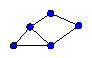
\includegraphics[width=\textwidth]{images/simple-graph.pdf}
		\caption{}
		\label{simplegraph}
	\end{subfigure}
	~
	\begin{subfigure}[b]{0.24\textwidth}
		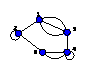
\includegraphics[width=\textwidth]{images/multi-graph.pdf}
		\caption{}
		\label{multigraph}
	\end{subfigure}
	~
	\begin{subfigure}[b]{0.22\textwidth}
		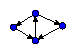
\includegraphics[width=\textwidth]{images/directed-graph.pdf}
		\caption{}
		\label{directedgraph}
	\end{subfigure}
	~
	\begin{subfigure}[b]{0.23\textwidth}
		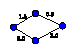
\includegraphics[width=\textwidth]{images/weighted-graph.pdf}
		\caption{}
		\label{weightedgraph}
	\end{subfigure}
	\caption{Classifications of graphs: (\subref{simplegraph}) A simple graph. (\subref{multigraph}) A graph with multiple edges and loops. (\subref{directedgraph}) A directed graph. (\subref{weightedgraph}) A weighted graph.}
	\label{fig:graphtypes}
\end{figure} 

\begin{rem} 
	In this  study, we will be working with simple connected undirected graphs or networks unless stated otherwise.\\
	\end{rem}
\begin{defn}[Subgraph]
	Given a graph $G=(V,E)$, we say $G'=(V',E')$ is a subgraph of $G$ if and only if $V' \subseteq V$ and $E' \subseteq E$. $G$ is called the supergraph \citep{estrada2015first}. \\ 
\end{defn}

\begin{defn}[Incidence]
	Given a graph $G=(V,E)$. We say that node $v$ and edge $e$ are incident if $v$ is one of the nodes to which edge $e$ connects. Two edges $e_1$ and $e_2$ are said to be incident if they share a vertex $v\in V$ \citep{newman2010networks}. \\
	%Formally, $\exists~ v \in V | v \in e_1 \cap e_2$ 
\end{defn}

\begin{defn}[Vertex adjacency]
	For a given network, two vertices $v_i$ and $v_j$ are adjacent if there exists an edge, $e$, connecting the two vertices, that is, $e = \{v_i,v_j\}$. With the understanding of adjacency, we can represent a network using a matrix known as adjacency matrix $\mathbf{A}$ \citep{newman2010networks}.\\
\end{defn}

\begin{defn}[Neighborhood ($N_G(v)$)]
	The neighborhood of a vertex $v \in V$ is a set of all vertices that are adjacent to $v$ \citep{newman2010networks}. Mathematically, $N_G(v) = \{u \in V \vert uv \in E \}$\\
\end{defn}

\begin{defn}[Degree of a node ($k_v$)]
	The degree of a vertex $v$ is the number of edges incident to it. A self-edge is counted as two edges. The degree of a node $v$ is the number of nearest neighbors of $v$, that is, $k_v = |N_G(v)|$. If $k_v = 0$, then node $v$ is said to be isolated in $G$, and if $k_v = 1$, then $v$ is a leaf of the graph. The minimum degree $k_{min}(G)= min\{k_v \vert v \in G\} $ and the maximum degree $k_{max}(G)= max\{k_v \vert v \in G\}$. For a directed network, we consider two types of degrees, namely in-degree ($k_v^{in}$) and the out-degree ($k_v^{out}$), which are the number of edges pointing towards or departing from a node $v$ respectively \citep{estrada2011structure}. The total degree $k_v$ is $k_v = k_v^{in}+ k_v^{out}$.\\
\end{defn} 

%\begin{lem}[Handshaking]
%	For any given undirected network $G=(V,E)$, the sum of all vertex degrees is equal to twice the number of edges \citep{newman2010networks}.
%	\begin{eqnarray}
%	\sum_{v\in V} k_v = 2~|E|.
%	\end{eqnarray}
%\end{lem}


\begin{defn}[Walk]
	A walk in a network is a series of edges (not necessarily distinct)
	\begin{eqnarray*}
		(u_1,v_1),(u_2,v_2),\ldots,(u_k,v_k),\quad \text{ for which }  v_i=u_{i+1} ~(i=1,2,\ldots,l-1).
	\end{eqnarray*}
	
	A trail is a walk in which all the edges are distinct \citep{estrada2015first}. A walk of length $k$ is referred to as a $k$-walk. We can compute the number of $k$-walks between any pair of nodes in a network using the entries of $\mathbf{A}^k$ where $\mathbf{A}$ is the Adjacency matrix of a graph which we discuss in subsequent subsections.\\
\end{defn}

\begin{defn}[Path]
	A path of length $l$ is a walk of length $l$ in which all the nodes and edges are distinct. A closed path is called a cycle \citep{estrada2011structure}. For any pair of nodes $v_i$,$v_j$ in a connected graph, there exists at least one path connecting $v_i$ to $v_j$. The paths with minimum length are referred as shortest-paths.\\
\end{defn}

\begin{defn}[Irreducible set of shortest paths]
	
	An irreducible set of shortest paths of length $l$ is the set $P_l ={P_l(v_i,v_j),P_l(v_i,v_r),\cdots, P_l(v_s,v_t)}$ in which the endpoints of every shortest-path $P_l(v_i,v_j)$ in the set are different.
	Each path in this set is referred to as an irreducible shortest-path \citep{estrada2012path}.\\
\end{defn}


\begin{defn}[Connectivity of a graph]
	A non-empty graph $G$ is said to be connected if there exists a path between any two pair of vertices (Diestel,2000). \\
\end{defn}

\begin{defn}[Connected component of a graph]
	A component of an undirected graph is a subgraph in which any two vertices are connected to each other by paths, and which is connected to no additional vertices in the supergraph \citep{newman2010networks}. 
	A connected component is also referred to as a maximal connected subgraph of a graph. \\
\end{defn}

Some special categories of graphs include:\\

\begin{defn}[Star graph]
	A star graph, denoted as $S_n$, is a complete bipartite network $K_{1,n}$ \citep{wilson1970introduction}.\\
\end{defn}

\begin{defn}[Complete graph]
	A graph $G = K_{V (G)}$ is a complete graph on $V(G)$, if every two nodes are adjacent: $E = E(G)$. We denote a complete network of order $n$ by $K_n$. \\
\end{defn}

\begin{defn}[Regular graph]
	A graph network is a graph $G$ in which every node has the same degree. A $k$-regular graph is one in which every node has degree equal to $k$.\\
\end{defn}

\begin{defn}[Cycle]
	A cycle graph is a connected graph in which there exists an edge connecting one node to another and each node has degree $2$. A cycle with $n$ nodes is denoted as $C_n$ \citep{wilson1970introduction}.\\
\end{defn} 

\begin{defn}[Bipartite]
	A network $G=(V,E)$ is bipartite if the nodes can be divided into disjoint sets $V_1$ and $V_2$ such that $(u,v) \in E$ implies that $u \in V_i$, $v \in V_j$, $i\neq j$. A  bipartite graph in which each node of $V_1$ is connected to each node of $V_2$ is known as a complete bipartite graph; if $|V_1|= m$ and $|V_2|= n$, such a graph is denoted by $K_{m,n}$ \citep{newman2010networks}. \\
\end{defn}

\begin{defn}[Tree]
	A tree is a connected undirected graph that contains no closed loops \citep{newman2010networks}. It is important to note that a tree with $n$ vertices has $(n-1)$ edges. A spanning tree of a graph $G=(V,E)$ is a subgraph of $G$ with vertex set $V$, which is a tree. $G$ has a spanning tree if and only if $G$ is connected. \\
\end{defn}

\begin{figure}[H]
	\centering
	\begin{subfigure}[b]{0.19\textwidth}
		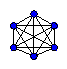
\includegraphics[width=\textwidth]{images/complete-graph.pdf}
		\caption{}
		\label{complete}
	\end{subfigure}
	~
	\begin{subfigure}[b]{0.19\textwidth}
		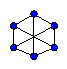
\includegraphics[width=\textwidth]{images/regular-graph.pdf}
		\caption{}
		\label{regular}
	\end{subfigure}
	~
	\begin{subfigure}[b]{0.20\textwidth}
		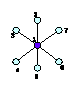
\includegraphics[width=\textwidth]{images/star.pdf}
		\caption{}
		\label{star-graph}
	\end{subfigure} ~
    \begin{subfigure}[b]{0.24\textwidth}
    	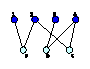
\includegraphics[width=\textwidth]{images/bipartite-graph.pdf}
    	\caption{}
    	\label{bipartite}
    \end{subfigure}
	\caption{ (\subref{complete}) A complete graph with $6$ nodes. (\subref{regular}) A $3$-regular graph. (\subref{star-graph}) A star graph, $S_6$. (\subref{bipartite}) A bipartite graph with $m=4$ and $n=3$.}
	\label{fig:compreggraphs}
\end{figure}

\begin{defn}[Network]
	A network is a diagrammatic representation of a system. It consists of nodes (vertices), which represent the entities of the system. Pairs of nodes are are joined by links (edges), which represent a particular kind of interconnection between those entities \citep{estrada2011structure}.
	\label{def:network}\\
\end{defn}
However, Definition \ref{def:network} does not exploit the different ways in which the nodes are connected and their directions. For instance, directed edges, self-loops and multiple edges. It is because of such issues that \citep{gutman2012mathematical} suggested definitions for a simple network as well as a more general definition of networks. First, let us understand the term `relation'.\\

\begin{defn}[Relation]
	Consider a finite set $V=\{v_1,v_2, \cdots,v_n \}$ of unspecified elements, and let $V \otimes V$ be the set of all ordered pairs $[v_i,v_j]$ of the elements of $V$.
	A relation on the set $V$ is any subset $E \subseteq V \otimes V$. The relation $E$ is symmetric if $[v_i, v_j] \in E$ implies $[v_j, v_i] \in E$ , and it is reflexive if $\forall~ v \in V$, $[v,v] \in E$. The relation $E$ is antireflexive if $[v_i,v_j] \in E$ implies $[v_i \neq v_j]$ \citep{estrada2011structure}.\\
\end{defn}

\begin{defn}[Network: More general definition]
	A network is a triple $ G = (V,E,f)$, where $V$ is a finite set of nodes, $E \subseteq V \otimes V = \{e_1,e_2,\cdots,e_m \} $ is a set of links, and $f$ is a mapping which associates some elements of $E$ to a pair of elements of $V$, such as that if $v_i \in V$ and $v_j \in V$, then $f: e_1 \rightarrow [v_i,v_j]$ and $f:e_2 \rightarrow [v_j,v_i]$. A weighted network is created by replacing the set of links $E$ by the set of link weights   
	$W=\{w_1,w_2,\cdots,w_m \}$, such that $w_i \in \mathcal{R}$ . Then, a weighted network is defined by $G=(V,W,f)$ \citep{estrada2011structure}.\\
\end{defn}



\subsection{Complex systems and complex networks}

Complex systems are very vital in our daily lives. They exist in fields such as social, economic, science, technology among others.  During his interview with San Jose Mercury News on January 23, 2000, Stephen Hawking referred to the $21$st century as a century of complexity \citep{Hawkinginterview}. 

Complex systems are composed of interconnected components, however, it has been observed that many complex systems display a behaviour phenomenon (also known as emergent behaviour) that cannot be explained by any conventional analysis of the system's constituent parts \citep{EncyBrit}. In otherwords, for one to understand the behaviour of a system, it is necessary for one to consider a holistic system-level view point. There are different approaches to study of complex systems for instance statistical description, empirical data analysis, simulations, analytical approach and network approach. 

In this work, we focus on the network approach in which we represent complex systems by complex networks whose nodes (vertices) and links(edges) represent the components and the interactions among components respectively.  For example, a transportation system can be represented by network where nodes are cities or towns and the links are the roads, railways or flight routes. This is then followed by mathematical formulation of the problem, modelling and validation.  

%	Second, is network analysis which entails studying the structure of the network from which the properties of the network (and the system) are drawn.  First, as Estrada \citep{estrada2015first} mentioned that complex networks are the skeletons of complex systems,
An interesting early historical application of the network approach to the study of complex systems is the K\"{o}nigsberg bridge problem which is described in \citep{euler1976solution,euler1953leonhard}. Euler solved the problem by reformulating it in terms of a graph where vertices represent islands while edges represent the seven bridges joining any two islands as shown in Fig~\ref{bridgeproblem}. Work published by Leonhard Euler \citep{euler1976solution} is considered the genesis of the story of network theory.

\begin{figure}[!h]
	\centering
	\begin{subfigure}[b]{0.45\textwidth}
		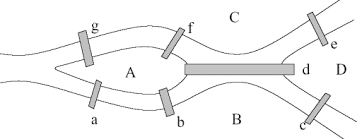
\includegraphics[width=\textwidth]{images/koningsberg.png}
		\caption{}
		\label{kornbridge}
	\end{subfigure}
	\qquad
	\begin{subfigure}[b]{0.19\textwidth}
		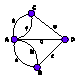
\includegraphics[width=\textwidth]{images/bridge-graph.pdf}
		\caption{}
		\label{bridgegraph}
	\end{subfigure}
	\caption{The K\"{o}nigsberg bridges: (\subref{kornbridge}) is a schematic diagram of the seven K\"{o}nigsberg bridges. (\subref{bridgegraph}) is a graph representing the K\"{o}nigsberg bridges. Source: \citep{bridgeimage}. }
	\label{bridgeproblem}
\end{figure} 


As the size of network increases from just graphs of tens or hundreds of nodes which could easily be analysed by direct use of eye so as to ascertain the structure of the network  to complex networks consisting of million or billion of nodes which call for advanced analytic approach that involves development of statistical methods to quantify such large networks. The statistical methods aid in answering questions such as how many nodes or edges should be removed for the network to break down, what  the shortest path length of the network is, and many others. 

%Some of the characteristics of complex systems include: emergent behaviour, self organisation, decentralised organisation of components, evolving nature of complex systems, among others.


\subsection{Examples of real-world networks}
Networks are used in many fields such as in biology, chemistry, computer science, transport, psychology, social sciences among others. For instance, in computer science, a network can be a representation of computers, routers, or any other electronic devices that are connected together by wires or wireless connections.
In his work \citep{newman2003structure}, Newman considered a loose categorisation of networks: social networks, communication networks, technological networks, and biological networks.
\begin{enumerate}[a.]
	\item Social Networks
	
	Networks considered as social networks are ones whose nodes correspond to people or groups of people while the edges represent the interactions or relationship between them \citep{jackson2010social}. For instance friendship networks such as facebook, twitter in which the interactions represent friendship ties among acquaintances, networks of intermarriages between families, social interaction networks which capture peoples' interactions through social activities or events, employee networks with companies, and many others.
	Some common networks that researchers have frequently experimented upon include: the Zachary karate network which consists of two communities centred at the administrator and instructor as a result of misunderstanding that prevailed with the karate club earlier on. The nodes in the network are the members of the club as the links represent interactions between members during non-club activities \citep{zachary1977information}. Other networks include the dolphin network \citep{williams1993abundance}, terrorist networks \citep{magouirk2008connecting}, among others .
	
	\item Information networks: 
	
	Information networks are also referred to as knowledge networks. Examples of networks under this category include: 
	The world wide web which consists of billions of web pages as nodes that are linked together through links known as hyperlinks \citep{huberman2001laws}.
	Another network categorised as information networks are citation networks that are composed of nodes which are articles while directed link between two nodes written as $i\longrightarrow j$ indicate article $i$ cites article $j$.
	\item Technological networks:
	
	This category consist of networks made by man to aid in distribution or transfer of resources, services or commodities such as electricity, water, transportation services, and many others. Examples of such networks include the internet, transportation networks, power grids, to mention but a few \citep{faloutsos1999power,pagani2013power,banavar1999size}.
	\item Biological networks: 
	
	Biological networks exists in areas related human and processes that take place with in the human body, animals and their ways of survival, chemistry. Such networks include the human brain network, protein-protein interaction network, network of metabolic path ways, ecological networks \citep{estrada2011structure,sporns2004organization,schwikowski2000network}.
\end{enumerate}
\begin{figure}[H]
	\centering
	\begin{subfigure}[b]{0.4\textwidth}
		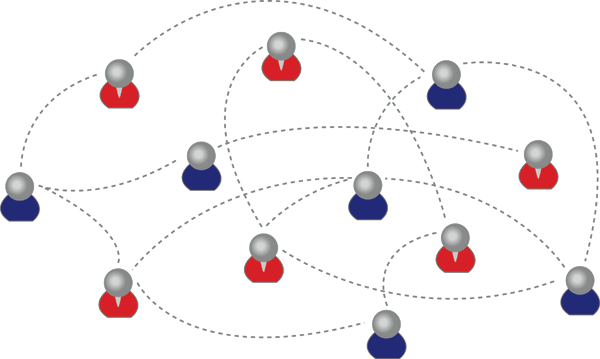
\includegraphics[width=\textwidth]{images/social-network_3.png}
		\caption{}
		\label{socialnetwork}
	\end{subfigure}
	\quad 
	\begin{subfigure}[b]{0.4\textwidth}
		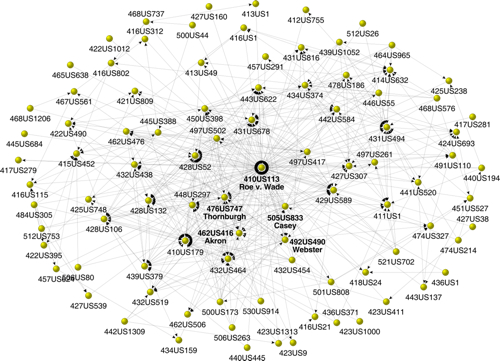
\includegraphics[width=\textwidth]{images/citation.jpg}
		\caption{}
		\label{citationntk}
	\end{subfigure}
	
	\begin{subfigure}[b]{0.4\textwidth}
		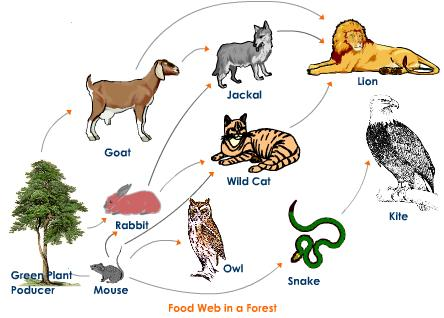
\includegraphics[width=\textwidth]{images/foodweb.jpeg}
		\caption{}
		\label{foodweb}
	\end{subfigure}
	\quad 
	\begin{subfigure}[b]{0.4\textwidth}
		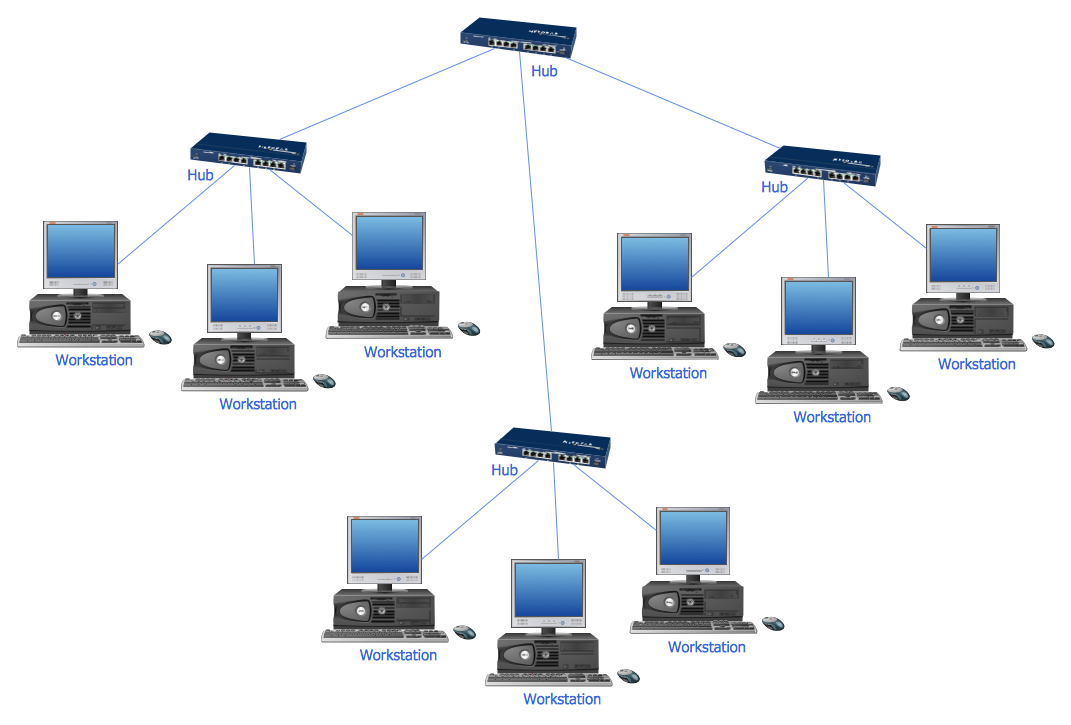
\includegraphics[width=\textwidth]{images/computer-2.png}
		\caption{}
		\label{internet}
	\end{subfigure}
	\caption{Networks in real world: (\subref{socialnetwork}) A social network. (\subref{citationntk}) A citation network. (\subref{foodweb}) A food web.  (\subref{internet}) Computer network. Source: \citep{googleimages}}
	\label{fig:Tree}
\end{figure} 



%\subsubsection{Characteristics of complex systems}
%\begin{enumerate}
%	\item Emergence
%	
%	Complex systems are emergent phenomena as they are the spontaneous outcome of the interactions among the many constituent units \citep{barrat2008dynamical}. Complex systems, unlike engineering systems, they are not formed based on a blue print. They instead evolve to form emergent architecture and they exhibit unexpected properties and characteristics.
%	\item Self organisation	
%	
%	Complex systems are characterised by self organising properties that are exhibited through the collective and unsupervised dynamics of the components of the system. The collective behaviour justifies the fact that one cannot understand the whole system and its dynamics by dismantling the system and studying each component in isolation. Taking the internet for example, there is no central authority responsible for controlling the addition of new computers(nodes) or connection lines (links) onto the network. Another example is the eco-system in which feeding pattern followed by animals is in no way controlled by any central agent. 
%	
%	\item No central organising mind
%	
%	In complex systems, it appears as though there exists a central control. However, in reality, control is spread over a decentralised structure that is to say system behaviour is due to the combination of the different components that make up the system \citep{EncyBrit}. This property of complex systems makes them resilient as failure of some of the components may not critically affect the functioning of the whole system.
%	
%	\item Uncertainty
%	
%	Complex systems exhibit an unpredictable kind of behaviour. For instance, in a transportation system of a city, opening new free ways may result into an increase in traffic jam.
%	
%	Other characteristics of complex systems include their evolving and adaptive nature. In addition, no conventional way can be used to describe complex systems.
%	%	\item Evolving
%	%	\item Adaptive
%	%	\item No conventional way of description
%\end{enumerate}

\subsection{Matrix representations of graphs}
Graphs can be represented in a number of ways namely edge lists, matrices, and many others. However, matrices are the most widely used technique for representation of graphs especially for large graphs whose structure cannot be captured by human eye. In addition, representing graphs by matrices enables the application of mathematical and computer tools on networks for purposes of summation, pattern identification and many others \citep{chandak2017novel,turan1984succinct}. In the subsequent subsections, we discuss the most common matrices used in the field of graph theory as well as their properties.

\subsection{Adjacency Matrix}
The Adjacency matrix is very useful and simple matrix commonly used in graph representation. It captures the connection between nodes in the graph that is to say, which node is connected to which one in the graph. The adjacency matrix (also known as binary adjacency) is square matrix whose entries are given by
\begin{eqnarray}
\mathbf{A}_{ij} = \begin{cases} 1 &\mbox{if } i \text{ and } j \text{ are adjacent}, \\
0 & \text{otherwise}.
\end{cases}
\end{eqnarray}
The summation of the $i$th row or column is equivalent to the total number of immediate neighbours, known as degree, of  vertex $v_i$. For simple undirected networks, the matrix is symmetric with zeros entries at the main diagonal. However, for directed networks, the matrix may be asymmetric since direction of edges have to be considered. For multigraphs, the entries  are the number of edges between each pair of vertices and for graphs with loops the diagonal entries are non-zero due to self-loops which may be counted once or twice based on whether the network is directed or undirected \citep{biggs1993algebraic,godsil2001algebraic}. For graphs with weighted edges, the adjacency matrix is given by 
\begin{eqnarray}
\mathbf{A}_{ij} = \begin{cases} w_{i,j} &\mbox{if } i \text{ and } j \text{ are adjacent}, \\
0 & \text{otherwise}.
\end{cases}
\end{eqnarray}


The spectrum, which is the eigenvalues and their multiplicities, of the Adjacency matrix is such a rich one and is thus used to mine interesting information about the graph. For example, the multiplicity of the largest eigenvalues is equal to the number of connected components of the graph \citep{cvetkovic2004spectral}. 

The summation of the absolute values of the eigenvalues of the adjacency matrix is referred to as the energy, $E$, of the graph. It is given by
\begin{equation}
E = \sum_{i} |\lambda_i|,
\end{equation}
where $\lambda_i$ is the $i$th eigenvalue of $\mathbf{A}$. The concept of energy of a graph has its origin in chemistry (by Gutman in 1978) where it is used in approximating the total $\pi$ electron energy of molecules \citep{gutman2001energy}. This concept has however been extended to other matrices resulting into different kinds of graph energy as discussed in \citep{ramane2008bounds,gutman2009incidence,gutman2006laplacian}


\subsection{Degree matrix}
	The degree matrix is a diagonal matrix that provides information about the degree of each node in a given network \citep{newman2010networks}. Given a network $G=(V,E)$ with $n=|V|$, the degree matrix $\mathbf{D(G)}$ is defined as
	\begin{eqnarray}
	D_{i,j} =  \begin{cases} k_i &\mbox{if } i = j \\
	0 & \text{otherwise}.
	\end{cases}
	\end{eqnarray}
	In a directed network the degree of node may be the in-degree or the out-degree.


\subsection{Distance matrix}
The distance matrix also known as the all-pairs shortest path matrix denoted by $\mathbf{S}$ is a symmetric matrix whose elements are defined as 
\begin{equation}
	S_{i,j} =  \begin{cases} l_{i,j} &\mbox{if } i \neq j \\
0 & \text{otherwise},
\end{cases}
\end{equation}
where $l_{i,j}$ is the length of the irreducible shortest path between nodes $i$ and $j$.

\subsection{Incidence matrix}
	Consider a network with vertex set $V=\{v_1,v_2, \cdots,v_n\}$ and edge set $E =\{e_1,e_2,\cdots,e_m \}$. Let us consider an arbitrary orientation of every edge in the network, say, we label each edge $\{v_i,v_j\}$ in a way that $v_i$ is the positive end and $v_j$ is the negative end. It should be, however, noted that the orientation does not matter. Then the oriented incidence matrix $\mathbf{B(G)}$ has entries defined as
	\begin{eqnarray}
	B_{ij} = \begin{cases} +1 &\mbox{if } \text{ node $v_i$ is the positive end of the edge } e_j \\
	-1 &\mbox{if }  \text{ node $v_i$ is the negative end of the edge } e_j\\
	0 & \text{otherwise}.
	\end{cases}
	\end{eqnarray}

\subsection{Laplacian Matrix}
The Laplacian matrix or graph Laplacian is one of matrices used to represent a graph or network. Recently, a number of researchers have been deeply involved in the study of the Laplacian matrix of a graph since this matrix has interesting spectral properties that provide more useful information about the structure of a graph as compared to other matrices such as the adjacency matrix. The Laplacian plays a key role as a natural link between discrete representations like graphs and continuous representations such as vector spaces and manifolds. 
There are various applications of the graph Laplacian which include spectral clustering, spectral matching, diffusion on networks, centrality measure, among others, which we explore later on. 

The Laplacian matrix takes on different versions namely the normalised and unnormalised Laplacian matrices.

\subsection{Definitions and properties of the Laplacian matrix}

\begin{defn}[Combinatorial Laplacian Matrix]
	The Combinatorial Laplacian or unnormalised Laplacian matrix of a network is defined as the difference between the Degree matrix $\mathbf{D}$ and the Adjacency matrix $\mathbf{A}$ of a network. That is,
	\begin{eqnarray}
	\mathbf{L} = \mathbf{D} - \mathbf{A}.
	\end{eqnarray}
	Given a simple network $G=(V,E)$, the entries of the combinatorial Laplacian matrix $\mathbf{L(G)}$  are defined as
	\begin{eqnarray}
	L_{ij} = \begin{cases} k_{v_i} &\mbox{if } i = j \\
	-1 &\mbox{if } i \neq j \text{ and } v_i \text{ is adjacent to } v_j \\
	0 & \text{otherwise},
	\end{cases}
	\end{eqnarray}
	where $k_{v_i}$  denotes the degree of node $i$ \citep{estrada2011structure}.
	
	Alternatively, we can define the combinatorial Laplacian matrix of a graph in terms of the vertex-edge incidence matrix $\mathbf{B}$. That is,
	\begin{eqnarray}
	\mathbf{L} =  \mathbf{B} \mathbf{B}^T,
	\label{lintermsb}
	\end{eqnarray}
	where $\mathbf{B}^T$ is the transpose of $\mathbf{B}$ \citep{estrada2011structure}.
\end{defn}

Some of the properties of the Combinatorial graph Laplacian  include the following:
\begin{enumerate}	
	\item{Real and symmetric matrix} 
	
	The entries of the Laplacian matrix are real numbers and are symmetric with respect to the main diagonal \citep{das2004laplacian}. Thus, the spectrum is real.
	\item{Singular matrix}
	
	The Laplacian matrix is a square matrix that is not invertible. Its determinant is equal to zero \citep{das2004laplacian}.
	\item{Positive semi-definite}
	
	A matrix is positive semi-definite if and only if all its eigenvalues are non-negative. For a given matrix $\mathbf{L}$, this property is denoted by $\mathbf{L}\geq 0$. This property of the Laplacian matrix makes it more suitable for spectral analysis compared to the adjacency and incidence matrices.
	
\end{enumerate}
\subsubsection{Spectrum of the combinatorial Laplacian matrix}
As mentioned earlier, the spectrum of the Laplacian provides useful information about the structure of a network. The spectrum of the Laplacian matrix is the set of all its eigenvalues and their multiplicities \citep{estrada2011structure}. Let $\lambda_1 < \lambda_2 < \ldots < \lambda_n$ be the distinct eigenvalues of $\mathbf{L}$ and let $m(\lambda_1),m(\lambda_2), \ldots,m(\lambda_n)$ be their multiplicities. Then, the spectrum of $\mathbf{L}$ is written as
\begin{eqnarray}
Sp\mathbf{L} = 
\renewcommand*{\arraystretch}{1.1}
\begin{pmatrix*}
\lambda_1 & \lambda_2 & \ldots & \lambda_n \\
m(\lambda_1) & m(\lambda_2) & \ldots & m(\lambda_n)
\end{pmatrix*}.
\end{eqnarray}

We consider the non increasing order of the eigenvalues of $\mathbf{L}$: $\lambda_n  \geq \lambda_{n-1} \geq  \cdots \geq \lambda_2 \geq \lambda_1 =0 $. Some of the results associated with the spectrum of the Laplacian matrix include:
\begin{itemize}
	\item The eigenvalues of $\mathbf{L}$ are bounded as 
	$ 0 \leq \lambda_j \leq 2k_{max} \quad \text{and} \quad \lambda_n \geq k_{max} $ \citep{estrada2011structure}.
	\item The eigenvalue $\lambda_1$ is always equal to zero \citep{estrada2011structure}. At least one eigenvalue of the Laplacian is $0$.
	\begin{proof}
		Consider the vector $v= (1/\sqrt{n}, \cdots, 1/\sqrt{n}) $. We know that the $i$th entry of $Lv$ is 
		
		$\sum_{i\sim j} v_{(i)}- v_{(j)} = \sum_{i\sim j} (1/\sqrt{n} - 1/\sqrt{n}) = 0 = 0 \cdot v_{(i)}$.
	\end{proof}
	%\item The smallest non-zero eigenvalue of $\mathbf{L}$ is called the spectral gap.
	\item The multiplicity of $0$ as an eigenvalue of $\mathbf{L}$ is equal to the number of connected components in the network \citep{estrada2011structure}.
	\item Every row sum and column sum of $\mathbf{L}$ is zero. Thus, the vector $\mathbf{v_1}$ of all ones is an eigenvector associated with $\lambda_1 =0$, since $\mathbf{Lv_1} = \mathbf{0} $ \citep{das2004laplacian}.
	\item  A network is connected if its second smallest eigenvalue is nonzero. That is, $\lambda_2> 0$ if and only if $G$ is connected. The eigenvalue $\lambda_2$ is thus called the algebraic connectivity of a network, $a(G)$. The magnitude of this value depicts how well connected the overall graph is. The algebraic connectivity has significant implications for properties such as clustering and synchronizability.
	The eigenvector corresponding to the eigenvalue $\lambda_2$ is called the Fiedler vector \citep{estrada2015first}.
	
	\item Let $G$ be a graph with $n$ connected components $G_i (1 \leq i \leq n)$. Then the spectrum of $G$ is the union of the spectra of $G_i$ (and multiplicities are added) \citep{brouwer2011spectra}.
	
	\item For a graph $G$, the sum of the eigenvalues, that is, the trace of $\mathbf{L}$ is twice the number of edges of $G$. Mathematically, $\sum_{i=1}^n \lambda_i = Trace(\mathbf{L}) = 2E.$ \citep{brouwer2011spectra}\\
\end{itemize}


\begin{thm}[Fiedler, 1975]
	Suppose $G = (V,E)$ is a connected network with graph Laplacian $\mathbf{L}$ whose second smallest eigenvalue is $\lambda_2 > 0$. Let $x$ be the eigenvector associated with $\lambda_2$. Let $r \in \mathbb{R}$ and partition the nodes in $V$ into two sets
	\begin{eqnarray}
	V_1 = \{i \in V|x_i \geq r\}, ~ V_2 = \{i \in V | x_i < r\}, 
	\end{eqnarray}
	then the subgraphs of $G$ induced by the sets $V_1$ and $V_2$ are connected \citep{estrada2015first}.
	\label{fiedler}\\
\end{thm}
This result is useful for partitioning a network while ensuring that all the parts remain connected. This method of partitioning using eigenvalues is known as spectral clustering. For clusters of equal size, we choose $r$ such that it is the median value of $x$. 


Some analytic expressions for the spectra of different kinds of simple networks are:
\begin{itemize}
	\item Star, $S_n$ : $Sp(\mathbf{L}) = \{ 0~ 1^{n-2}~n\}$. 
	
	\item Complete, $K_n$ : $Sp(\mathbf{L}) = \{ 0~ n^{n-1} \}$. 
	
	\item Complete bipartite, $K_{m,n}$ : $Sp(\mathbf{L}) =\{ 0 ~ m^{n-1} ~ n^{m-1}\}$ \citep{estrada2011structure}.\\
	
\end{itemize}

\begin{thm}[Kirchoff's Matrix-Tree Theorem]
	If $G$ is a connected graph with Laplacian matrix $\mathbf{L}$, then the number of unique spanning trees of $G$ is equal to the value of any cofactor of the matrix $\mathbf{L}$ \citep{harris2008combinatorics}.
	\label{thm:kirchoff}
\end{thm}

\subsection{Normalized Laplacian matrix}
One format of normalized Laplacian matrix also known as symmetric normalised Laplacian is defined as 
\begin{eqnarray*}
	\mathcal{L}_{ij} = \begin{cases} 1, &\mbox{if } i = j \text{ and } k_i \neq  0, \\
		- \frac{1}{\sqrt{k_i k_j}}, &\mbox{if } v_i \text{ and } v_j \text{ are adjacent,} \\ 
		0, & \text{otherwise}.
	\end{cases}
\end{eqnarray*}

We can also write 

\begin{eqnarray*}
	\mathbf{\mathcal{L}} = \mathbf{D}^{-1/2} \mathbf{L} \mathbf{D}^{-1/2} = \mathbf{I} -\mathbf{D}^{-1/2} \mathbf{A} \mathbf{D}^{-1/2}
\end{eqnarray*}
where $\mathbf{D}^{-1/2}$ is the diagonal matrix determined by the inverse square root of each diagonal entry of the degree matrix \citep{estrada2011structure}. For a $k$-regular graph, we have
\begin{equation}
\mathcal{L} = \mathbf{I}-\frac{1}{k} \mathbf{A}.
\end{equation}

The matrix $\mathcal{L}$ is symmetric with real and nonnegative eigenvalues which satisfies:
\begin{equation*}
0  = \lambda_1(\mathcal{L}) \leq  \lambda_2(\mathcal{L}) \leq \cdots \leq  \lambda(\mathcal{L}) \leq 2.
\end{equation*}
It is very convenient to work with the spectrum of the normalised Laplacian because of the small interval ($[0,2]$) for example it is easier to compare the spectrum of the normalised than the unnormalised Laplacian of two graphs. In addition, the eigenvalues of the normalised Laplacian are consistent with the eigenvalues in spectral geometry and in stochastic processes. Using this spectrum, results that were only known for regular graphs can be extended to general graphs \citep{chung1997spectral}. It is for these reasons that we will, in most cases, consider the normalised version of the Laplacian.
The largest eigenvalue, $\lambda_n(\mathcal{L})$, is equal to $2$ only for a bipartite graph. Like the combinatorial Laplacian, the smallest eigenvalue is zero and its the multiplicity is equal to the number of connected components of the corresponding graph. 

For a graph $G$ with $n$ vertices, $\sum_{i}\lambda_i(\mathcal{L}) \leq n$ and inequality only holds when $G$ consists of isolated vertices.

\subsection{Random walk normalised Laplacian}
This variant of the Laplacian matrix is based on the random walks in the graph. It is an unsymmetric matrix defined as 
\begin{equation}
\mathbf{L}_r = \mathbf{L} D^{-1}
\end{equation}
The relationship between $\mathbf{L}_r$ and $\mathcal{L}$ is :
\begin{equation}
\mathbf{L}_r = \mathbf{D}^{1/2} \mathbb{L} \mathbf{D}^{-1/2}.
\label{randomNorm}
\end{equation}
By diagonalizing $\mathcal{(L)}$, Eqn.\ref{randomNorm} can be rewritten as 
\begin{equation}
\mathbf{L}_r = (\mathbf{D}^{1/2} \mathbf{\Phi}) \mathbf{\Lambda} (\mathbf{D}^{1/2} \mathbf{\Phi})^{-1},
\label{decomprandom}
\end{equation}
where $\mathbf{\Lambda}$ is a diagonal matrix of eigenvalues of $\mathcal{(L)}$ and $\mathbf{\Phi}$ is the eigenvector matrix. Thus, $\mathbf{L}_r$ can is diagonizable and it shares the same set of eigenvalue as $\mathcal{L}$ though the corresponding eigenvectors are different. From this relationship, some applications would use the random matrix $\mathbf{L}_r$ in place of $\mathcal{(L)}$.

A detailed account of other variants of the Laplacian matrix can be found in \citep{tsiatas2012diffusion}.

\subsection{Randi\'{c} matrix}
Let $G=(V,E)$ be a graph with vertex set ${v_1,v_2, \cdots, v_n}$. Let $d_i$ denote the degree of a vertex $v_i$. The entries of the Randi\'{c} matrix (name proposed in \citep{bozkurt2010randic}) are given by
\begin{equation*}
\mathbf{R}_{ij} = \begin{cases} 0, &\mbox{if } i = j \\
\frac{1}{\sqrt{k_i k_j}}, &\mbox{if } v_i \text{ and } v_j \text{ are adjacent} \\ 
0, & \text{otherwise}.
\end{cases}
\end{equation*}
The sum of all elements of $\mathbf{R}$ is $2R$, where $R$ is known as the Randi\'{c} index. This index has numerous applications in chemistry with a historical one being its usage as a molecular structure descriptor, introduced by Milan Randi\'{c} \citep{randic1975characterization}.

The Randi\'{c} matrix is related to the symmetric normalised Laplacian matrix by
\begin{equation}
\mathcal{L} = \mathbf{I} -\mathbf{R},
\end{equation}

Let $p_i$ denote the $i$th eigenvalue of $\mathbf{R}$, then 
$\lambda_i (\mathcal{L}) = 1- p_i$. Moreover, for a graph without isolates, the Randi\'{c} energy (given by $E_{R}(G) = \sum_{i} p_i$) is equal to the combinatorial normalised Laplacian energy ( given by $ E_{\mathcal{L}} (G) = \sum_{i} \lambda_i (\mathcal{L})$).

\subsection{Transition matrix of a random walk on a Graph}
It is an $n \times n$ matrix $\mathbf{P}_G$ whose entries are given by
\begin{equation}
\mathbf{P}_{ij} = \frac{1}{k_i} \mathbf{A}_{ij},
\end{equation}
In other words, $\mathbf{P}_G = \mathbf{D}_{G} ^ {-1} \mathbf{A}$ which is the normalised adjacency matrix.

The entry at $\mathbf{P}_{ij}$ indicates the probability for a random walker moving from vertex $i$ to $j$. Like any other stochastic matrix, the eigenvalues of $\mathbf{P}$ are such that $|\lambda_i(\mathbf{P})| \leq 1$.

The transition matrix is normally encountered in the study of Markov chains where its spectrum is used to compute the time it takes for the chain to reach its stationary distribution (mixing time) as discussed in \citep{behrends2000introduction}.

%\section{Characteristics of Networks}


\section{Structure of a network}

The structure of a network is a description of how nodes are connected to each other in a network. 
The study of network structure for purposes of understanding and predicting properties of networks was first and much embraced by chemists who used graphs to represent chemical molecules where vertices are used to represent atoms and edges to represent chemical
bonds.  In their work \citep{brown1868connection}, Crum Brown and Fraser were among the earliest researchers who put forward the idea that the properties of a chemical molecule are greatly dependent on its structure.  This structure-property relationship has further been explored using graph-theoretical approach not only in chemistry but in other fields such as social networks, biological networks and many others \citep{mihalic1992graph,smith2004associations,wellman1988social,wey2008social}.  

As pointed out in previous chapters, complex networks are used to represent complex systems. The behaviour exhibited by complex systems is due to the interconnectedness between system components not individual components. In order to understand behaviour and properties of these system, we need to study the structure of the corresponding networks from which we deduce properties of the networks from which the behaviour of the systems can be drawn. Let us discuss some of the properties that characterise the static structure of a network, that is where the interconnections between nodes remain constant with time:

\subsection{Average degree of the nearest neighbors}
The average degree of the nearest neighbor of a vertex $i$ is given by
\begin{equation}
k_{nn,i} = \frac{\sum_{j=1}^{n} a_{ij} k_j}{k_i},
\end{equation}
where $a_{ij}$ is the $(i,j)$th element of the adjacency matrix and $n$ is the number of nodes in the network.
This measure checks the correlation between the degrees of different vertices.

\begin{defn}[Distance between a pair of nodes]
	In a network, the distance $d_{ij}$ between two nodes, labelled $i$ and $j$ respectively, is defined as the length of the shortest path (or geodesic path) connecting them \citep{wang2003complex}. It is also known as geodesic distance. It is possible to have more than one shortest path between a pair of nodes.\\
\end{defn}

\begin{defn}[Diameter of a network]
	The diameter of a network is the maximum distance between any two
	nodes in the network \citep{wang2003complex}. The diameter of a graph $G= (V,E )$ is defined as \[ \text{diam}(G ) = \max_{i,j \in V} d_{ij}.\] For a disconnected network, the diameter is undefined and therefore, for such a case, we take the efficiency.
\end{defn}	

\begin{defn}[Efficiency]
	The efficiency, $\bar{e}$, of a network is a measure defined as
	\begin{eqnarray*}
		\bar{e} =\frac{1}{n(n-1)} \sum_{i,j \in V,i\neq j} \frac{1}{d_{ij}},
		\label{eqn:eff}
	\end{eqnarray*}
\end{defn}
where $d_{i,j}$ is the shortest path between vertices $i$ and $j$, and $n$ is the size of the network.

The efficiency of a network is a measure of how efficiently information spreads between vertices, thus networks with high values of efficiency are considered fast spreaders of information and a large percentage of vertices are reached compared to their counterparts with lower values of efficiency.\\

\begin{defn}[Average path length]
	The average path length of a network is the average number of steps along the shortest paths for all possible pairs of network nodes. Let $G = (V , E )$ be a graph the average path length $L_G$ is defined by
	\begin{eqnarray}
	L_G = \frac{1}{n(n-1)} \sum_{i,j \in V,~i \neq j} d_{ij},
	\end{eqnarray}
	where $d_{ij}$ is the shortest path between node $i$ and $j$ and $n$ is the total number of nodes in $G$. The value of $L$ determines the size of a network and helps to determine the efficiency of information flow or disease spread over a network \citep{wang2003complex}.
\end{defn}

\subsection{Clustering coefficient}
The clustering coefficient is a measure of the degree to which nodes tend to cluster together. Such behaviour is more evident in real-world networks, especially social networks where nodes tend to form tightly knit groups that have relatively high density of ties among them \citep{estrada2015first}.
Consider three nodes in a network, say, $i$, $j$ and $k$. Suppose $i$ is connected to both $j$ and $k$ (two neighbors of a node will be neighbors themselves), then the likelihood that $j$ and $k$ are also connected is what is known as the clustering coefficient. In other words, clustering coefficient measures the density of triangles in a  network. 
The value of the clustering coefficient is in the interval $[0,1]$. There are two types of clustering coefficients namely, the local and the global clustering coefficients.\\

\begin{defn}[Local clustering coefficient]
	The local clustering coefficient is a measure of the clustering tendency in a node's immediate network. The local clustering coefficient for a node $i$ with degree $k_i$ is formally defined as 
	\begin{eqnarray}
	C_i = \frac{\text{number of pairs of neighbors of } i\text{ that are connected}}{\text{number of pairs of neighbors of }i}= \frac{2 t_i}{k_i(k_i-1)},  
	\end{eqnarray}
	where $t_i$ is the number of triangles attached to node $i$. For nodes with degree equal to zero or one, we set $C_i = 0$ since there are no triangles attached to such nodes \citep{newman2010networks}. The average clustering coefficient for the network is given by
	\begin{eqnarray}
	\bar{C} = \frac{1}{n} \sum_i C_i.\\
	\end{eqnarray} 
\end{defn}

\begin{defn}[Global clustering coefficient]
	The global clustering coefficient is concerned with the density of triplets of nodes in a network. A triplet is defined as three nodes that are connected by either two (open triplet) or three (closed triplet) ties. Global clustering coefficient determines the overall level of clustering in a network \citep{opsahl2009clustering}.
	Mathematically, we define the global clustering coefficient $C$ as
	\begin{eqnarray}
	C = \frac{3 \times \text{number of triangles}}{\text{number of connected triplets of vertices}} = \frac{\sum t_\vartriangle}{\sum t},
	\end{eqnarray}
	where $\sum t_\vartriangle$ is the total number of closed triplets and $\sum t$ is the total number of connected triplets of vertices in the network.
\end{defn}

\subsection{Degree distributions}
The scattering of node degrees over a network is characterised by the distribution function, $p(k)$, which is the probability that a node chosen uniformly at random has degree $k$. We define $p(k)$ to be the fraction of nodes in a network that have degree $k$. That is, $p(k) = n(k)/n,$ where $n(k)$ is the number of nodes with degree $k$ in a network of size $n$. The degree distribution of a network is  referred to as the probability distribution of node degrees over that network. It is represented by plot of $p(k)$ against $k$ \citep{estrada2011structure}. Fig.~\ref{distribution} is of plots of some of the common degree distributions in networks namely Gaussian, Poisson, exponential and power-law degree distributions.

%\begin{exa} We compute the degree distribution for the network in Fig.~\ref{deg-distb}.
%	
%	\begin{figure}[H]
%		\centering
%		\begin{minipage}[t]{.30\textwidth}
%			\centering
%			\vspace{0pt}
%			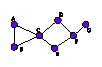
\includegraphics[width=\textwidth]{images/degree-prob.pdf}
%			\captionof{figure}{A network of size $7$.}
%			\label{deg-distb}
%		\end{minipage}
%		\hfill
%		\begin{minipage}[t]{.64\textwidth}
%			\centering
%			\vspace{0pt}
%			\captionof{table}{Degree distribution of nodes in network in Fig.~\ref{deg-distb}.}
%			\setlength{\tabcolsep}{15pt}
%			\renewcommand{\arraystretch}{1.2}
%			\begin{tabular}{|c|c|c|}
%				\hline 
%				Node & Degree, $k$ & $p(k)$ \\
%				\hline
%				G & $1$ & $1/7$ \\
%				A,B,D,E & $2$ & $4/7$ \\
%				F & $3$ & $1/7$ \\
%				C & $4$ & $1/7$ \\
%				\hline
%			\end{tabular}
%		\end{minipage}
%	\end{figure}
%\end{exa}
%
%We use the degree distribution of a network to obtain useful insights about the structure of a network. The structure of a network is a description of how nodes are linked to each other to form a network. It is important to note that networks with different structures can have the same degree distribution which implies that degree distribution gives us some but not all the information regarding the structure of a network. Thus, we cannot deduce a complete structure of a network based on information about its degree distribution alone. Fig.~\ref{distribution} shows some of the common degree distributions in networks.

\begin{figure}[H]
	\centering
	\begin{subfigure}[b]{0.45\textwidth}
		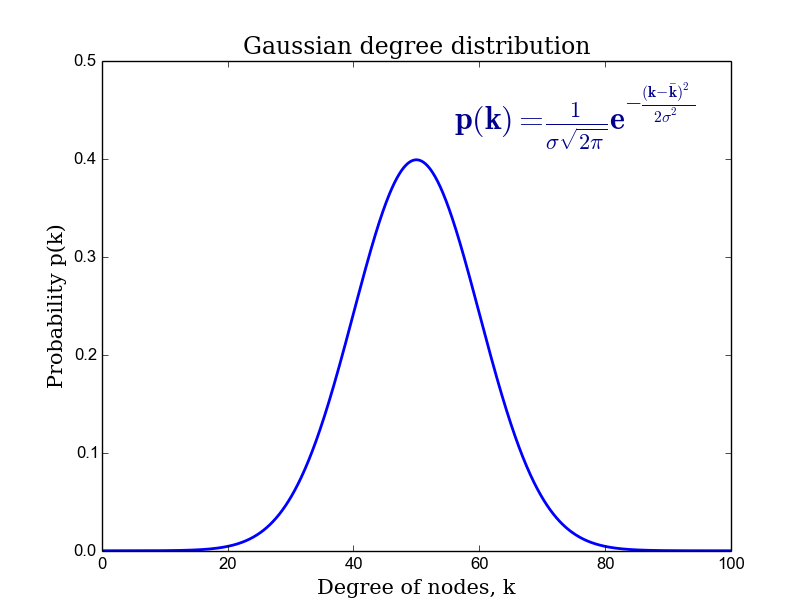
\includegraphics[width=\textwidth]{images/gaussian.png}
		\caption{}
		\label{gauss}
	\end{subfigure}~ 
	\begin{subfigure}[b]{0.45\textwidth}
		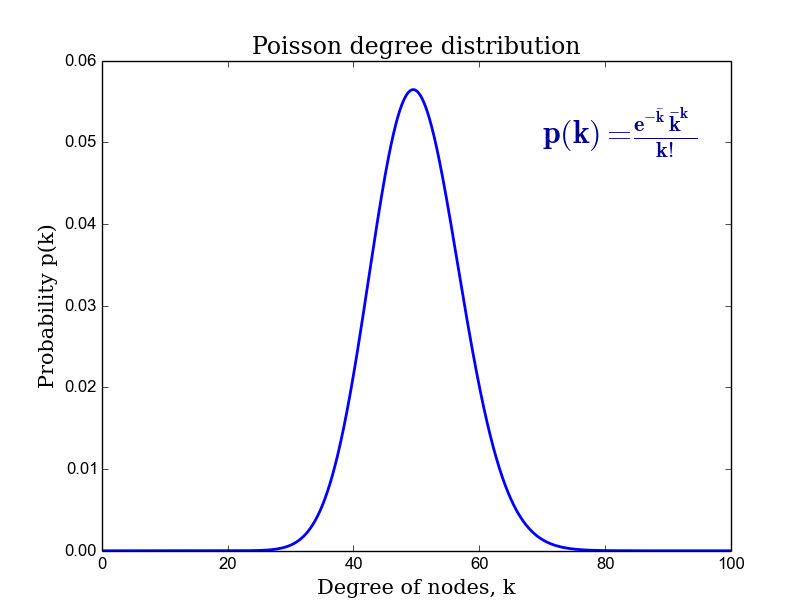
\includegraphics[width=\textwidth]{images/pois.png}
		\caption{}
		\label{poss}
	\end{subfigure} \\   
	\begin{subfigure}[b]{0.45\textwidth}
		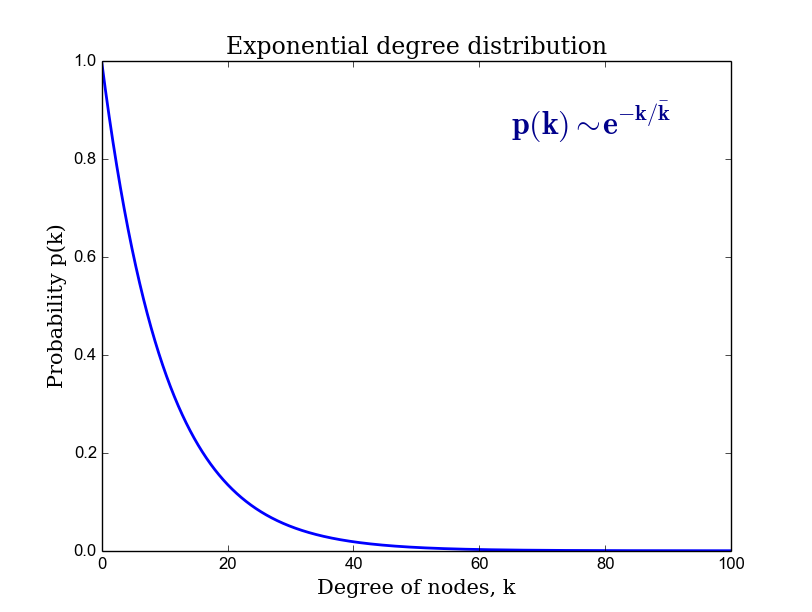
\includegraphics[width=\textwidth]{images/exp.png}
		\caption{}
		\label{expo}
	\end{subfigure}~
	\begin{subfigure}[b]{0.45\textwidth}
		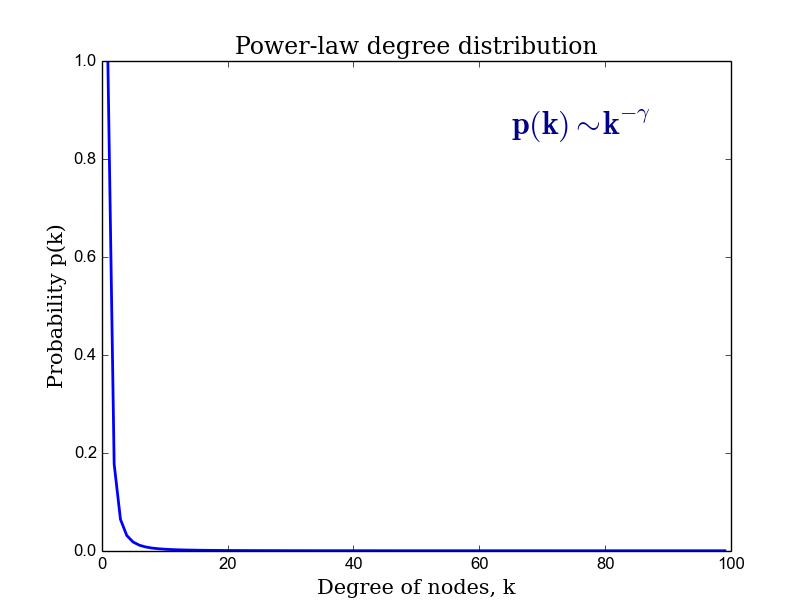
\includegraphics[width=\textwidth]{images/p-law.png}
		\caption{}
		\label{powerlaw}
	\end{subfigure}
	\caption{Common degree distributions of networks: (\subref{gauss}) Gaussian distribution. (\subref{poss}) Poisson distribution. (\subref{expo}) Exponential distribution.(\subref{powerlaw}) Power-law distribution.}
	\label{distribution}
\end{figure} 

\subsubsection{Power-law degree distribution}
In the power-law degree distribution, there exists few nodes with very high degree and many with very low degree. In otherwords, the probability of finding a node with degree $k$ decreases as a negative power of degree $k$. This implies that in such networks, it is less likely to find a node with high degree \citep{estrada2011structure}.
Formally,
\begin{eqnarray}
p(k) = C k^{-\gamma}, \text{ for } 2 \leq \gamma  \leq 3.
\label{eqn:power-law}
\end{eqnarray}

The range of the exponent between $2$ and $3$ was asserted by Barab\'{a}si in Linked \citep{barabasi2003linked}. However, other literature indicate an exponent of grater than zero (that is, $\gamma > 0$).

Using a logarithmic scale, the plot of Equation (\ref{eqn:power-law}) is a straight line, $\ln p(k) = -\gamma \ln k + \ln C $, with a slope equal to $-\gamma $ and an intercept equal to $\ln C$ as illustrated in Fig.~\ref{log-plots}(\subref{noisy}). However, we observe that the part that corresponds to high degrees (tail of the distribution) is very noisy. In order to overcome this problem, one of the solutions is to consider the cumulative distribution function, which is defined as 
\begin{eqnarray*}
	P(k) = \sum_{k'=k}^\infty p(k'),
\end{eqnarray*}
which represents the probability of randomly choosing a node with degree $k$ or greater \citep{estrada2011structure}. The plot of cummulative distribution function on a logarithmic plot is a straight line as shown in Fig.~\ref{log-plots}(\subref{cdf}).

\begin{figure}[H]
	\centering
	\begin{subfigure}[b]{0.38\textwidth}
		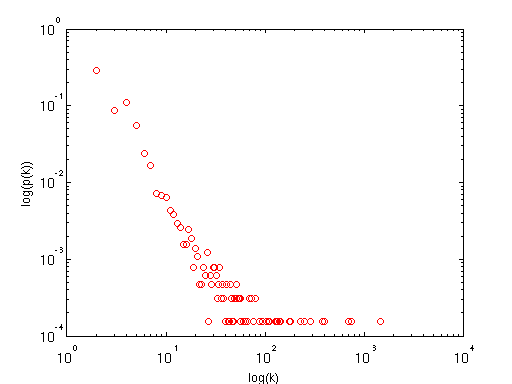
\includegraphics[width=\textwidth]{images/noisyplot.png}
		\caption{}
		\label{noisy}
	\end{subfigure}
	~ 
	\begin{subfigure}[b]{0.38\textwidth}
		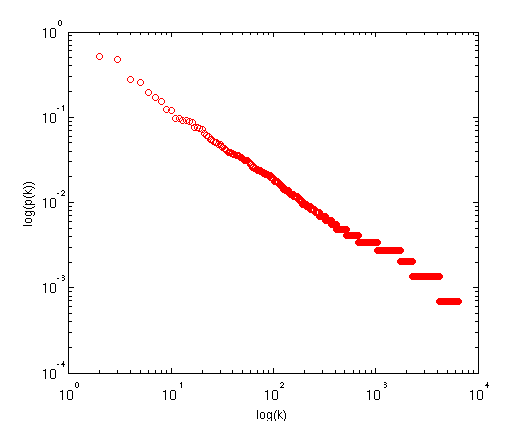
\includegraphics[width=\textwidth]{images/cfdplot.png}
		\caption{}
		\label{cdf}
	\end{subfigure}
	\caption{ Probability (\subref{noisy}) and Cummulative Distribution Function (\subref{cdf}) logarithmic plots for the version of the internet at autonomous system level (where anetwork or a collection of networks that are all managed and supervised by a single entity or organization) following a power-law distribution.  Source: \cite{frankthesis}. }
	\label{log-plots}
\end{figure}

When we scale the degree by a constant factor $a$, we obtain
\begin{eqnarray}
p(k,a) = C(ak)^{-\gamma} = a^{-\gamma} p(k) \propto p(k).
\label{scale}
\end{eqnarray}
Thus, scaling by a constant $a$ multiplies the original power-law relation by the constant $a^{-\gamma}$ which implies that all power laws with a particular scaling factor are scaled versions of each other. Thus, networks that follow a power-law distribution are referred to as scale-free networks.

In network science, there is an ambiguity in language regarding what 'scale free' really means. Some possible suggestions of what a scale free network is include: a network with power degree distribution with exponent in range $2$ to $3$, a network formed by the process of preferential attachment, one that follows a power law on some scales or one that does so throughout, and many others. 

Work published by Barab\'{a}si and his then graduate student R\'{e}ka Albert \citep{banavar1999size} claimed that many real world networks (such as genetic networks and world-wide web) have node connectivities that follow a scale free power law degree distribution. They further explained the observed degree distribution is attributed to the mechanism of formation of these networks known as preferential attachment (also known as rich-get-richer phenomenon) in which a new node coming into the network would most likely get connected to existing high-degree nodes (known as hubs) other than low-degree nodes. However, some researchers pointed out that preferential attachment is not the only mechanism that can be used in modelling networks that follow power law \citep{colman2013complex}. They further drew insights to the fact that networks can have the same power laws but different topologies. Moreover, this work triggered a multitude of publications affirming the existence of scale-freeness in biological, social, and many other real world networks \citep{jasny2003life,alon2003biological,cohen2002all,bray2003molecular}.

The claim that scale free networks are universal has been criticised by some network scientists and experts. For example, the scale freeness of some networks such as the power networks and metabolic networks has been questioned \citep{tanaka2005scale,amaral2000classes}. The most recent and so far the most debatable criticism was raised by Clauset and Broido in \citep{broido2018scale} where they asserted that scale free networks are rare in nature not contrary to what was claimed earlier on. They based their argument on statistical analysis of nearly $1,000$ networks from social, technological, biological and many other fields. Results from their result indicate that only about $4\%$ of the networks qualified highly with strongest direct evidence of scale-freeness in their structure and only $33\%$ exhibited weak levels of direct evidence of scale free structures. On considering a relaxed criteria where indirect evidence of scale free structure in networks was checked, only $53\%$ of the networks datasets passed the statistical tests in \citep{broido2018scale}. A very interesting debate on this issue is still on going as captured in \citep{Quantamagazine}, however, this posses an opportunity for research into this area.



\subsubsection{Structure of network and its degree distribution}
The degree distribution of a graph provides useful insights about its structure though it is not conclusive as 
graphs with different structures can have the same degree distribution which implies that degree distribution gives us some but not all the information regarding the structure
of a graph. Thus, in most cases, we cannot deduce a complete structure of a network based on knowledge of
its degree distribution. To further backup this argument, we consider a simple example of two graphs both of size $5$ (Figs. \ref{samedeg1} \& \ref{samedeg2}) and whose degree distribution is the same (see table \ref{tabdegdist}). We then compute some of the structural properties of the two graphs (as in table \ref{table-properties}) to ascertain whether their structures are the same.

\begin{figure}[H]
	\centering
			\begin{subfigure}[b]{0.35\textwidth}
				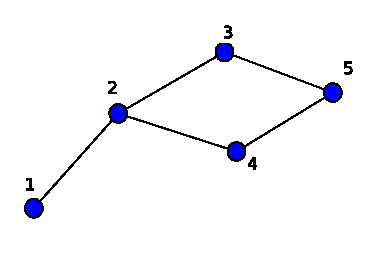
\includegraphics[width=\textwidth]{images/sameDegreeDistribution.pdf}
				\caption{}
				\label{samedeg1}
			\end{subfigure}~
			\begin{subfigure}[b]{0.35\textwidth}
				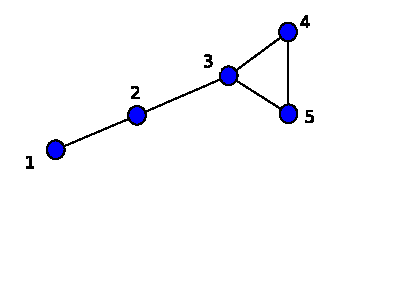
\includegraphics[width=\textwidth]{images/sameDegreeDistribution2.pdf}
				\caption{}
				\label{samedeg2}
			\end{subfigure}~ 
	\begin{subfigure}[b]{.35\textwidth}
		\centering
		\vspace{0pt}
		\setlength{\tabcolsep}{10pt}
		\renewcommand{\arraystretch}{2.0}
		\begin{tabular}{|c|c|}
			\hline 
			Degree, $k$ & $p(k)$ \\
			\hline
			$1$ & $1/5$ \\
			$2$ & $3/5$ \\
			$3$ & $1/7$ \\
			\hline
		\end{tabular}
        \caption{}	
        \label{tabdegdist}
	\end{subfigure}
    \caption{Two simple graphs (\subref{samedeg1} and \subref{samedeg2}) of size $5$ both have the same degree distribution given in table (\subref{tabdegdist}).}
\end{figure}

\begin{table}[H]
	\centering
	\renewcommand{\arraystretch}{1.2}
	\begin{tabular}{|l|c|c|}
		\hline
		&G1 & G2 \\
		\hline
		\multirow{5}{*}{Average neighbour} & $1:3.0$ & $1: 2.0$\\
		& $2: 1.7$ & $2:2.0$\\
		& $3: 2.5$ & $3:2.0 $ \\
		& $4: 2.5$ & $4:2.5 $ \\ 
		& $5: 2.0$ & $5:2.5 $ \\
		\hline
		Diameter & 3 & 3 \\
		\hline
		Average Degree & 1.6 & 1.7 \\
		\hline
		Clustering Coefficient & 0 &0.4667 \\
		\hline
		Global efficiency & 0.7333 & 0.7167 \\
		\hline
	\end{tabular} 
    \captionof{table}{Some of the structural properties of the two graphs (Figs. \ref{samedeg1} \& \ref{samedeg2} ) whose degree distribution is the same. }  
    \label{table-properties}
\end{table}

Table \ref{table-properties} contains some of the selected structural properties computed for the two graphs. First, the average neighbor degree for the $5$ nodes for both graphs is different for example the average neighbor degree for node labelled $1$ in graphs $G1$ and $G2$ is  $1.20$ and $1.30$ respectively. The diameter, however, of both graphs is the same. On the other hand, other properties such as average degree, clustering coefficient and global efficiency have different values for both graphs. For example graph $G1$ has clustering coefficient of $0$ yet graph $G2$  has a value of $0.4667$. From the two values, we can tell that the structure for the two graphs is different.
We can thus conclude that we cannot totally rely on the similarity in degree distribution for both graphs to deduce that the graphs under study are structurally similar since other structural properties indicate otherwise.

\subsection{Network Heterogeneity}
The heterogeneity of a network is the irregularity characterised by the existence of a nodes with degree significantly larger than the average degree of the network \citep{estrada2010quantifying,albert2002statistical,newman2003structure}. The star network is considered the most heterogeneous for which the average degree tends to two as the number of nodes increases. On the other hand, the regular networks is considered the least heterogeneous as all nodes have the same degree, that is to say, regular networks are homogeneous. 

From the degree distribution, we can obtain some useful insights about the heterogeneity of a network. However, this technique may not perform well some cases. For example situation where more than one degree distribution fits for a given network, comparison of between two networks with totally different degree distributions, among others. To work around such cases, various measures that uniquely quantify network homogeneity have been put forward \citep{bell1992note,albertson1997irregularity,estrada2010quantifying}. 


\subsection{Random models of networks}
In the study of real-world networks (such as protein-protein interaction, transport network, food web, etc.), we observe different topological structures of these networks and it is of great importance to understand the mechanisms that are responsible for such structures. We therefore discuss some of the models that mimic real-world networks.
%Let us consider a network formed randomly by taking a collection of $n$ nodes and a pair of nodes $v$ and $u$ with a certain probability $p$. This we do for all $n(n-1)/2$ possible links. If we consider a fixed set of network parameters and that the links are created randomly, then we can create models that are known as random models \citep{estrada2011structure}Some of the most popular random models are discussed below.
\subsubsection{The Erd$\ddot{\text{o}}$s-R\'{e}nyi (ER) model}

This type of random model was introduced by Erd$\ddot{\text{o}}$s and R\'{e}nyi in $1959$. It is the best known model for random networks. In this model, we take $n$ isolated nodes and then fix a probability $p$ with which we link the nodes. For each pair of nodes, we generate a random number, $r$, uniformly from $[0,1]$. If $p>r$, the two nodes are connected forming a network. Networks generated by the ER model have a small average path length and their average clustering coefficient tends to zero as $n$ increases \citep{estrada2011structure}.
%\begin{itemize}
% \item The expected number of edges per node $\bar{m}$ is given by
%$\bar{m} = \frac{n(n-1)p}{2}$.
%\item The node degree $\bar{k} = (n-1)p$.
%\item For a large $n$, the probability $p(k)$ follow a Poisson distribution given by $p(k) = \frac{e^{-\bar{k}} \bar{k}^k}{k}$. 
%\item The average clustering  of the ER networks is $\bar{C} = p = \frac{\bar{k}}{n}$. The value of $\bar{C}$ is less than one which implies that large ER networks have no clustering at all since as $n$ increases the $\bar{C}$ tends to zero.
%\end{itemize}
\subsubsection{The Barab\'{a}si-Albert (BA) model}

Most of the real-world networks follow a power-law degree distribution. This  distribution was not manifested in ER networks and thus, Barab\'{a}si and Albert introduced a network model that generates networks that mimic the degree distribution observed in the real-world networks. This model uses a preferential attachment, or
rich get richer, mechanism to evolve a given initial graph. The preferential attachment technique involves an initial network with $n_0$ nodes, and at each step, a new node is introduced and connected to the existing nodes with a probability proportional to their degrees (or connectivity). The resulting networks are scale-free and have high clustering coefficients \citep{estrada2011structure}. 

\subsubsection{The Watts-Strogatz (WS) model}

An experiment carried out by Stanley Milgram in 1967 \citep{milgram1967small} consisted of randomly selected people in the cities of Omaha and Wichita in the United States of America (USA) who were asked to send letters to target persons living in Boston. The individuals at the starting points were asked to send the letters to persons they knew. Despite the fact that the senders and their respective targets were separated by more than $2000$km and that there was a total of $200$ million inhabitants in the USA by then, results showed that the letters took an average of about six steps to reach the targets and that there was a large group interconnection where an acquaintance of an individual fed back into his own circle, thus eliminating new contacts. In terms of networks, two properties are observed: the former implies a small average path length of $6$ while the latter implies a high clustering coefficient. It is from this experiment that the phrase "six degrees of separation" was born. This phrase explains a small world in which an individual is connected to another by a maximum of six steps. In 1998, \cite{watts1998collective} proposed a model that reproduces the two properties mentioned previously. This model starts with a circulant (or ring) network with $n$ nodes connected to $k$ nearest neighbors. With a fixed probability $p$, an end to each original link is rewired to a new randomly selected node. The WS model interpolates between a regular and a random network as shown in Fig.~\ref{rewire-process}(\subref{rewire-fig}). The intermediate network is a small-world with high clustering coefficient and a very small average path length. 

\begin{figure}[!h]
	\centering
	\begin{subfigure}[b]{0.6\textwidth}
		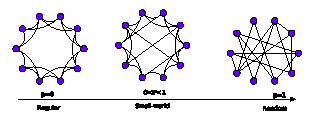
\includegraphics[width=\textwidth]{images/circular-graph.pdf}
		\caption{}
		\label{rewire-fig}
	\end{subfigure}~
	\begin{subfigure}[b]{0.42\textwidth}
		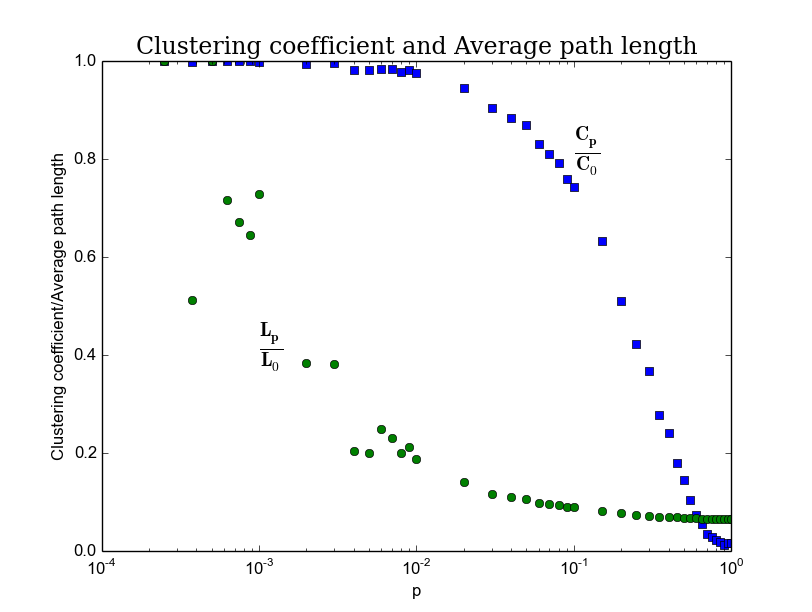
\includegraphics[width=\textwidth]{images/clus-pathlength.png}
		\caption{}
		\label{cluster-average}
	\end{subfigure}
	\caption{The rewiring process: (\subref{rewire-fig}) Interpolation of WS model as probability increases. (\subref{cluster-average}) Illustration of the variation of clustering coefficient and average path length during the rewiring process. }
	\label{rewire-process}
\end{figure}

In Fig.~\ref{rewire-process}(\subref{cluster-average}), as the probability increases during the rewiring process, the average path length and clustering coefficient vary. The region where the average path length is small and the clustering coefficient is high corresponds to the small world network in Fig.~\ref{rewire-process}(\subref{rewire-fig}).

In this study, we will perform simulations on networks developed by the ER and BA models using the following functions implemented in NetworkX:
\begin{verbatim*}
nx.gnp_random_graph(n,p,seed=None)
nx.barabasi_albert_graph(n,m,seed=None),
\end{verbatim*} 

where $n$, $p$, and $m$ are the number of nodes, the probability for edge creation, and number of edges to attach from a new node to existing nodes respectively. The argument seed (an integer) is the seed for random number generator.

\subsection{Robustness of complex systems}
	A complex systems is considered robust if it can withstand failures or perturbations that is to say a system can still perform as expected even in circumstances of failure of one or more components in the system. 
	In other words, robustness intuitively deals with the existence of back-up possibilities. In a network, this can be captured in the existence of alternative paths with in the network.\\
	
	 Robustness of systems plays an important role in a number of fields for instance in Engineering, understanding robustness acts as a basis for designing communication, transportation systems, power grids that can perform basic operation despite failure of some system components. In biology, robustness explains why some mutations lead to diseases while others do not. For ecologists and environmental experts, robustness helps in predicting the failure of an ecosystem when faced with disruptive human behaviours. In general, study of system robustness aids in understanding system operation, improving system performance and designing of new robust systems. \\
	 
	As mentioned earlier, the study of a network or graph underlying a complex system provides insights about the properties and characteristics of that systems. Thus, Barab\'{a}si \citep{barabasi2016network} highlighted the fact that networks play a vital role in robustness of complex systems which implies that exploring robustness of the network reflects that of the system.
	 
	\subsection{Robustness measures in networks}
	According to Ellens \citep{ellens2013graph}, robustness of a network is its ability to perform well when subject to failures or attacks. The attacks take on two forms namely: random attacks and targeted attacks. However, in order to tell whether a particular network is robust, there is need for a measure that quantifies the robustness. In the past, various robustness measures have been put forward by researchers \citep{sydney2008elasticity}. We explore some measures of robustness in networks which are categorised as follows:
	\subsubsection{Connectivity-based measures}
	Here we consider robustness measures that are based on the connectivity of the network. These include the classical connectivity $\kappa$, edge connectivity $\kappa_e$, and vertex connectivity $\kappa_v$. Firstly, the classical connectivity $\kappa$ is a measure whose value $\kappa=1$ for graphs in which there is a path between any pair of vertices that is connected graphs and $\kappa=0$ for unconnected graphs that is graphs in which atleast one pair of vertices  for which no path exists between them. Secondly, the edge connectivity $\kappa_e$ and vertex connectivity $\kappa_v$ are respectively the minimum number edges and vertices that need to be removed to disconnect the graph. The inequality $\kappa_v \leq \kappa_e \leq \delta_{min}$ holds for non-complete graphs, where $\delta_{min}$ is the minimum degree of vertices in a graph.
	\subsubsection{Distance-based measures}
	\begin{enumerate}
		\item Diameter
	
		The diameter of a graph, denoted as $D$, is the maximum distance between pairs of nodes in the graph\citep{wang2003complex}. The diameter of a graph $G= (V,E )$ is defined as \[ D = \max_{i,j \in V} \{d_{ij}\},\] where $d_{ij}$ is the shortest path between node $i$ and $j$. Based on the diameter, a graph is considered more robust if it's diameter is shorter.
		\item Average Path Length
		
		The average path length of a network is the average number of steps along the shortest paths for all possible pairs of network nodes. Let $G = (V , E )$ be a graph the average path length $L_G$ is defined by
		\begin{eqnarray}
		L_G = \frac{1}{n(n-1)} \sum_{i,j \in V,~i \neq j} d_{ij},
		\end{eqnarray}
		where $d_{ij}$ is the shortest path between node $i$ and $j$ and $n$ is the total number of nodes in $G$ \citep{wang2003complex}. 
		On comparing the average path length and diameter as measures of robustness, the former is considered a better measure as it strictly decreases on addition of edges which is not necessarily the case with the latter.
		\item Efficiency
		
		We can observe that we cannot compute the robustness of disconnected graph based on the two distance-based measures discussed previously. However, this is a possibility when we adopt the efficiency measure. 
		The efficiency of a graph, $E$ is defined as
		\begin{eqnarray}
			E =\frac{1}{n(n-1)} \sum_{i,j \in V,i\neq j} \frac{1}{d_{ij}}.
			\label{eqn:eff}
		\end{eqnarray}
		It is important to note that these measures based on distance consider only shortest path distances which implies that other alternative paths are not put into consideration which is a disadvantage for that matter.
	\end{enumerate}
	
	%\subsubsection{Reliability Polynomial}
	
	\subsubsection{Spectral graph measures}
	\begin{enumerate}
		\item Algebraic connectivity
		
		Given the spectrum of the Laplacian matrix of a graph $G$ in which the eignvalues are arranged in non-decreasing order: $0=\lambda_1\leq \lambda_2 \leq \cdots \leq \lambda_n$. The algebraic connectivity is the second smallest eigenvalue $\lambda_2$ of the Laplacian. It is the most common measure of robustness. The algebraic connectivity is equal to zero if and only if the graph is disconnected. The one disadvantage of this measure is the fact that it does not necessarily capture the addition of edges to a graph, that is to say, the value of $\lambda_2$ does not strictly increase on edge addition which implies that this measure is insensitive to edge addition in some cases.
		\item Number of spanning trees
				
		A spanning tree is a subgraph containing $n-1$ edges and no cycles. According to the Kirchoff's Matrix-Tree Theorem, the number of unique spanning trees, $\xi$, of graph $G$ is equal to the value of any cofactor of the Laplacian \citep{harris2008combinatorics}. It  is given by
		\begin{equation}
		\xi = \frac{1}{n} \prod_{i=2}^{n} \lambda_i.
		\end{equation}
		Baras and Hovareshti suggest the number of spanning trees as a global indicator of network robustness to edge removal. It has been proved that for $p$ close to zero, the number of spanning tree gives similar results for robustness as the reliability polynomial \citep{baras2009efficient}.
		
		Let us consider a simple example in which we illustrate how the both the algebraic connectivity behaves on edge addition. 
		\begin{figure}[!h]
			\centering
			\begin{subfigure}[b]{0.3\textwidth}
				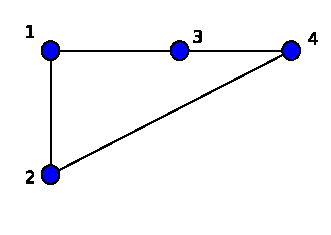
\includegraphics[width=\textwidth]{images/lap-algebraic.pdf}
				\caption{}
				\label{algebraic1}
			\end{subfigure}~
			\begin{subfigure}[b]{0.3\textwidth}
				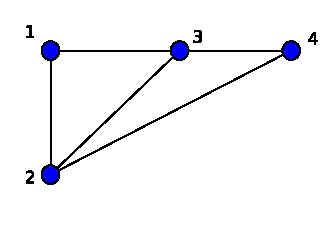
\includegraphics[width= \textwidth]{images/lap-algebraic2.pdf}
				\caption{}
				\label{algebraic2}
			\end{subfigure}
			\caption{The simple network in (\subref{algebraic1}) has algebraic connectivity $\lambda_2 = 2$. Adding a new edge,$e_{2,3}$ to form a network in (\subref{algebraic2}) with algebraic connectivity $\lambda_2 = 2$. We observe that on a change in network through edge addition, the algebraic connectivity remains constant.}
			\label{}
		\end{figure}
	
		\item Effective resistance
		
		The effective graph resistance $R$, also called total effective resistance or Kirchhoff index, is
		defined as the sum of the effective resistances over all pairs of vertices. It can be expressed in terms of the non-zero eigenvalues of Laplacian as
		\begin{equation}
		R = \sum_{1\leq i < j \leq n} R_{i,j} = n \sum_{i=2}^{n} \frac{1}{\lambda_i}
		\end{equation}
		Unlike the algebraic connectivity, the effective resistance involves not only one but all the non-zero eigenvalues of the Laplacian. It is for this reason that any changes due to edge addition or removal are captured which makes the latter a better measure of robustness.
		\item Natural connectivity
		
		This spectral measure of robustness was put forward by Wu et al.\citep{wu2564spectral}. It captures the core of robustness that is the capturing of redundancy of alternative paths. This is achieved by quantifying the weighted number of walks of all lengths in the graph. Closed walks are related to subgraphs of a graph for instance a closed walk of length $k=3$ represents a triangle. The number of closed walks of all lengths is obtained following the principle used in the computing the subgraph centrality as in \citep{estrada2011structure} in which the shorter closed walks have more influence than their longer counterparts. The penalisation entails dividing the sum of closed walks of length $k$ by the factorial of $k$. That is,  
		\begin{equation}
		S = \sum_{k=0}^{\infty} \frac{n_k}{k!},
		\label{sumclosed}
		\end{equation} 
		where $n_k$ is the number of closed walks of length $k$. We also know that,
		\begin{equation}
		n_k = trace(\mathbf{A}^k) = \sum_{i=1}^{N} \lambda_{i} ^k,
		\end{equation}
		where $\lambda_i$ is the $i$th largest eigenvalue of $\mathbf{A}(G)$.
		Substituting for $n_k$ in Eqn.\ref{sumclosed} gives
		\begin{equation}
		S = \sum_{k=0}^{\infty} \sum_{i=1}^{N} \frac{\lambda_{i} ^k} {k!} =  \sum_{i=1}^{N}\sum_{k=0}^{\infty} \frac{\lambda_{i} ^k} {k!}= \sum_{i=1}^{N} e^{\lambda_i}.
		\label{sumexpn}
		\end{equation}
		From Eqn. \ref{sumexpn}, we observe two facts. First, the weighted sum of closed walks can be obtained from the spectrum of the Adjacency matrix of a graph. second, the sum $S$ will be a large number for large $N$ and  thus the need to scale $S$. The scaled version of $S$, termed as the 'average eigenvalue' and denoted by $\bar{\lambda}$  is given by
		\begin{equation}
		\bar{\lambda} = \ln \big( \frac{S}{N}\big) = \ln \Big( \frac{\sum_{i=1}^{N} e^{\lambda_i}}{N} \Big).
		\end{equation}
		Unlike the algebraic connectivity, the natural connectivity changes monotonically when edges are added or deleted which is one of the desired properties of a robustness measure.
	\end{enumerate}

     \subsection{Graph similarity}
     Graph similarity has a wide range of applications such as web searching, chemical structure matching, comparing biological networks, synonym extraction, image clustering, social network mapping among others \citep{zager2008graph, nikolic2012measuring}. 
     The notion of graph similarity can be defined in many different ways based on the application for instance similarity of graphs can be based on whether graphs are identical copies of each other (isomorphism), how much the neighbourhood of a given node in one graph is similar to neighbourhood of a given node in the other graph, how much changes (node or edge deletion, redirection or addition) can be performed to one graph to obtain the other graph, among others \citep{zager2008graph}. Based on different definitions of similarities, measures of similarity can be categorised as follows.
     \begin{enumerate}
     	\item \textbf{Isomorphism based techniques}
     	
     	 Two graphs are isomorphic if there exists a bijective (one-to-one and onto) function between the sets of nodes
     	such that two nodes are connected in one graph if and only if their images under the bijection are connected \citep{zager2008graph}. In otherwords, two graphs are isomorphic if they are structurally identical. Graph isomorphism from $G$ to itself is known as graph automorphism. Formally, an automorphism of a graph $G = (V,E)$ is a permutation $\sigma$ of the vertex set $V$, such that the pair of vertices $(u,v)$ form an edge if and only if the pair $(\sigma(u),\sigma(v))$ also form an edge for example, vertex-transitive graphs are graphs for which any pair of vertices $u$ and $v$, there is an edge-preserving isomorphism mapping $u$ to $v$. Fig.~\ref{isomorphism} is an example of two isomorphic graphs.
     	
     	\begin{figure}[H]
     		\centering
     		\begin{subfigure}[b]{0.35\textwidth}
     			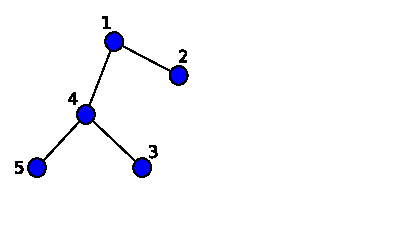
\includegraphics[width=\textwidth]{images/graph-isomorphism1.pdf}
     			\caption{}
     			\label{isomorphic1}
     		\end{subfigure}
     		\begin{subfigure}[b]{0.35\textwidth}
     			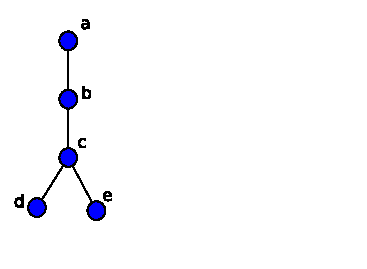
\includegraphics[width=\textwidth]{images/graph-isomorphism2.pdf}
     			\caption{}
     			\label{isomorphic2}
     		\end{subfigure} 
     		\caption{Two simple isomorphic graphs} 
     		\label{isomorphism}
     	\end{figure}
     Two graphs are similar if they are isomorphic, or they have isomorphic subgraphs (minimum or maximum common subgraphs) for which the larger the subgraph then the greater the similarity between the two graphs, or if one graph is isomorphic to a subgraph of another graph (subgraph isomorphism). Subgraph isomorphism can be used in image analysis to ascertain whether a given object is part of another object or a group of objects for instance in scenery study. Detailed algorithms for the three similarity measures can be found in \citep{weinberg1966simple,levi1973note,ullmann1976algorithm}
     
     Alternatively, another known technique is graph edit-distance (considered a generalisation of graph isomorphism) which involves transforming one graph into another by performing edit operations such as edge or node deletions, additions or substitutions, among others. Each operation is associated with a cost and the sequence of operations with the minimum cost is attained which amounts to a measure of similarity between the two graphs \citep{gao2010survey}.
     
     \item \textbf{Feature extraction}
     
     These are statistical methods that measure graph similarity based on properties of graph structure such as degree distribution, betweeness measures, diameter, eigenvalues and many others. Graphs are counted similar if their respective aggregated properties are assessed based on certain similarity measures and similarity is established. This method is very powerful as it maps graphs to various statistics that are smaller and easier to work with compared to original graphs. However, one draw-back of this method is the choice of the statistics which at times may not give intuitive results. Take an example of graphs with different number of nodes but with the same diameter, these graphs may be considered similar which is not actually true.
     
     \item \textbf{Iterative methods}
     
     These methods are based on the idea that two nodes are similar if their neighbourhoods are similar. The methods involve iterative processes in which nodes share similarity scores at each iteration until convergence is attained. A detailed review of some of the algorithms can be obtained in  \citep{jeh2002simrank,melnik2002similarity,zager2008graph}
     \end{enumerate}
     In this work, we use the concept of graph similarity as a basis for performing clustering (also known as graph clustering) on a given set of graphs extracted from objects. Here, we aim at grouping graphs into classes such that graphs belonging to the same class are similar and those belonging to different classes are dissimilar. In the subsequent subsection, we explore some of the key concepts we will encounter when extracting graphs from objects.
    %\subsection{Subgraph Matching}   
 
     \subsection{The Harris corner point detector}
     The detection of feature points in an image is vital in a number of tasks such as object tracking, $3$D scene reconstruction from stereo image pairs and many other tasks in machine vision \citep{trajkovic1998fast}. Though various algorithms for corner detection which are now considered state of the art, in this study we are interested in the Harris corner detection for demonstrating a principle of application and also since we are building on the earlier work of \citep{xiao2009graph,stoica2011delaunay}. Moreover, the algorithm could also be applied in this and other settings.
     
     The Harris corner point detector was introduced by Harris and Stephens \citep{harris1988combined} as an improvement to the Moravec's corner detector \citep{moravec1979visual,moravec1980obstacle}. In his method, Moravec considered corner points as the points where there is intensity variation in all directions. The Harris corner detector is widely used because it is simple to compute, fast and most importantly, the corner points obtained based on this method are invariant in position to rotation, scale, illumination, and partially to affine intensity changes as discussed in detail in \citep{stoica2011delaunay}. On the other hand, the Harris corner detector is not invariant to image scaling, however, there are various ways of going about this problem as explained in \citep{stoica2011delaunay}.
     
     The Harris Corner Detector method determines the nature of the point by computing the average change of intensity in the image when shifting a small local window in the image by small amount in any direction. For instance for a flat region, all shifts of the window result in very small changes in intensity, for an edge, a shift in the perpendicular results into a large change while for corner points, all shifts result into a large change in intensity. For a given image with intensities, $I$, a change due to a shift of a window $w$ of size $u,v$ by $(x,y)$ is given by \citep{stoica2011delaunay}
     \begin{equation}
     E_{x,y} = \sum_{u,v} w_{u,v} |I_{x+u, y+v} - I_{u,v}|^2,
     \end{equation}
     where $E$ is the change due to the shift, $x$ and $y$ are the window's displacements in the $x$ and $y$ directions respectively, $I$ is the intensity of image at a position $(u,v)$, and $w$ is the Gaussian window function  $e^{-\frac{u^2 + v^2}{2 \sigma^2}}$.
     
     The Taylor expansion of $E$ gives:
     \begin{equation}
     E_{x,y} = \sum_{u,v} \{[I_x (u,v)x]^2 + [I_y(u,v)y]^2 + 2I_x(u,v)I_y (u,v)xy\},
     \end{equation}  
     where $I_x = \partial I / \partial x$ and $I_y = \partial I /\partial y$. $E$ is a close approximation of the local autocorrelation function given by
     \begin{equation}
     E(x,y) = \mathbb{M}\begin{bmatrix}
     x & y
     \end{bmatrix} \Bigg(\sum_{u,v} w(u,v)  
     \begin{bmatrix}
     I_x ^2 & I_x I_y  \\
     I_xI_y & I_y ^2
     \end{bmatrix}  \Bigg)\begin{bmatrix}
     x \\
     y
     \end{bmatrix}  = \begin{bmatrix}
     x & y
     \end{bmatrix} \mathbb{M}\begin{bmatrix}
     x \\
     y
     \end{bmatrix}
     \end{equation}
     Matrix $\mathbb{M}$ describes the shape of the local autocorrelation function $E$ at the origin.
     Let $\lambda_1$ and $\lambda_2$ be the eigenvalues of $\mathbb{M}$, according to \citep{harris1988combined}, the measure of corner and edge quality used for selecting core pixels known as the response function, denoted as $R$ is given by
     \begin{equation}
     R = det(\mathbb{M}) - kTrace(\mathbb{M})^2,
     \end{equation}       
     where $det(\mathbb{M})=\lambda_1 \lambda_2$, $Trace(\mathbb{M}) = \lambda_1+ \lambda_2$ and $k$ is an empirical constant such that $0.04 <k < 0.06$.
     A corner region with $R>0$ is selected as a nominated corner pixel only if its response is an $8$-way local maximum.
     
     A clear step-by-step algorithm and Matlab code for the Harris corner Detector can be reviewed \citep{stoica2011delaunay}.\\
     
     \subsection{Voronoi diagrams and Delaunay triangulation} 
     \subsubsection{Voronoi diagrams }  
     Voronoi diagrams (also called Voronoi tessellations, Voronoi
     decompositions, or Dirichlet tessellations) are important geometrical structures that are found almost everywhere in the world. They have a wide range of applications such as modeling of biological structures such as cells, study of growth patterns of forests and forest canopies in ecology, tracing sources of infections in epidemics, finding clear routes in autonomous robot navigations, among others \citep{okabe2009spatial}. However, in later chapters, we will explore the application of Voronoi diagrams to image segmentation as explained in \citep{stoica2011delaunay}.\\
     \begin{defn}
     	A Voronoi diagram is a special kind of decomposition of a metric space (or plane) into regions based on distances to a specified discrete set of objects in the space (usually denoted by a
     	set of points normally referred to as seeds, sites or generators), according to the nearest-neighbor rule, such that each point is associated with the region of the plane closest to it \citep{aurenhammer2000voronoi}. The regions are referred to as Voronoi cells. The Voronoi vertices are the vertices of a complex formed from a set of all Voronoi cells and their faces. In other words, a Voronoi vertex is the common boundary of 3 adjacent cells. The Voronoi edge, on the other hand, is the common boundary of two adjacent cells.
     \end{defn}
     One simple and practical example that also doubles as an application of voronoi diagrams. Let us consider $n$ ambulances placed at different spots of a city. The spots are a subset of points denoted by $S = {p_1, p_2, \cdots, p_n}$. We assume that the distance between two points is given by the Euclidean distance function:
      \begin{equation}
      \ell_2 = d[(a_1,a_2),(b_1,b_2)] = \sqrt{(a_1 -b_1)^2 + (a_2 -b_2)^2}.
      \end{equation} Suppose other factors remain constant and that the nearest ambulance is contacted in cases of emergency, then the area to be served by an ambulance located at spot $p_k$ is given by the region $R_k$ around point $p_k$.
      
      Before we go any further, we first discuss some of the definitions used in the study of Voronoi diagrams as by ref \cite{aurenhammer2000voronoi}:
      \\
      \begin{defn}[Convex Set]
      	In a Euclidean space, a convex region (or set) is a region where, for every pair of points within the region, every point on the straight line segment that joins the pair of points is also within the region.\\
      \end{defn}
 
      \begin{defn}[Convex Hull]
      	The convex hull (or convex envelope) of a set $P$ of points in the Euclidean plane or in a Euclidean space is the smallest convex set that contains $P$.\\
      \end{defn}
       \begin{defn}[Simplex]
       	A $k$-simplex is a k-dimensional polytope (a geometric object with flat sides) which is the convex hull of its $k+1$ vertices.\\
       \end{defn}
       \begin{defn}[Planar graph]
       	A planar graph is a graph that can be drawn in the plane without any edges crossing. A planar graph drawn in this way divides the plane into regions bounded by the edges of the graph. These regions are called faces. \\
       \end{defn} 
       \begin{defn}[Dual graph]
       	The dual graph $G^*$ of a plane graph $G$ is a plane graph whose vertices correspond to the faces of $G$ and whose edges correspond to the edges of $G$.\\
       \end{defn}
      
      Voronoi diagrams exhibit interesting properties which include the following:
      \begin{itemize}
      	\item The closest pair of points corresponds to two adjacent cells in the Voronoi diagram.
      	\item Assume the setting is the Euclidean plane and a group of different points are given. Then two points are adjacent on the convex hull if and only if their Voronoi cells share an infinitely long side.
      	\item The Voronoi diagram on $n$ points (or sites) is a planar graph with $n$ faces and by Euler's formula for planar graphs: $v-e+n=2$ ( where $v$, $e$, and $n$ are the number of vertices, edges and faces of a planar graph respectively), the number of Voronoi vertices and edges are atmost $2n-5$ and $3n-6$ respectively. The time complexity is $O(n \log{n})$.
      	\item Each point on an edge of the Voronoi diagram is equidistant from its two nearest neighbors $p_i$ and $p_j$. Thus, there is a circle centered at such a point such that $p_i$ and $p_j$ lie
      	on this circle, and no other site is interior to the circle.
      	\item It follows that vertex at which three Voronoi cells $V(p_i)$, $V(p_j)$, and $V(p_k)$ intersect is equidistant from all sites. Thus it is the center of the circle passing through these sites, and this circle contains no other sites in its interior.
      	\item If we assume that no four points are co-circular, then the vertices of the Voronoi diagram all have degree three.
      	
      \end{itemize}
  
      
      \subsubsection{Delaunay triangulation}
      Let $P={p_1, p_2, \hdots,p_n} \subset \mathbb{R}^2$ be a point set. A triangulation $\mathcal{T}$ of $P$ is a maximal planar subdivision with vertex set $P$. Following the Empty circle property, $\mathcal{T}$ is a Delaunay triangulation of $P$ if and only if the circumcircle of any triangle in $\mathcal{T}$ does not contain a point of $P$ in its interior \cite{aurenhammer2000voronoi}. Delaunay Triangulation have been applied in various fields for example climate and global modeling \citep{ju2011voronoi}, modeling computer vision problems \citep{dinas2014review}, and many others.
      
      There are various methods of computing the Delaunay Triangulations namely: plane sweeping, iterative flipping from any other triangulation, randomized incremental construction, and conversion from Voronoi diagram. For this work, however, we will consider the Voronoi diagram based method. For a Euclidean space with point sites, the dual graph of the Voronoi diagram corresponds to the Delaunay Triangulation whose vertices are the point sites. 
      Delaunay triangulations have interesting properties which include the following:
      \begin{itemize}
      	\item Circum-circle property: The circum-circle of any triangle in the Delaunay triangulation
      	is empty that is it contains no sites of $P$.
      	\item Empty circle property: Two sites $p_i$ and $p_j$ are connected by an edge in the Delaunay
      	triangulation, if and only if there is an empty circle passing through $p_i$ and $p_j$.
      	\item Closest pair property: The closest pair of sites in P are neighbors in the Delaunay triangulation.
      	\item Given a point set $P$ with $n$ sites where there are h sites on the convex hull, in the plane, the Delaunay triangulation has $2n – 2 – h$ triangles, and $3n – 3 – h$ edges.
      	\item The exterior face of the Delaunay triangulation is the convex hull of the
      	point set.
      \end{itemize}
       
       
       
      \begin{figure}[H]
      	\centering
      	\begin{subfigure}[b]{0.30\textwidth}
      		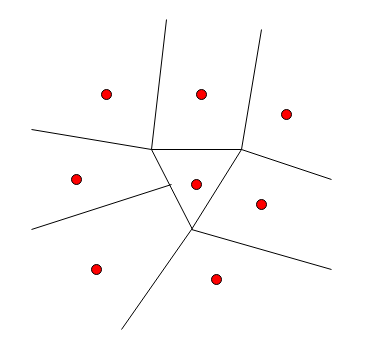
\includegraphics[width= \textwidth]{images/VoronoiDiagram.png}
      		\caption{}
      		\label{VoronnoiDiag}
      	\end{subfigure}~
      	\begin{subfigure}[b]{0.30\textwidth}
      		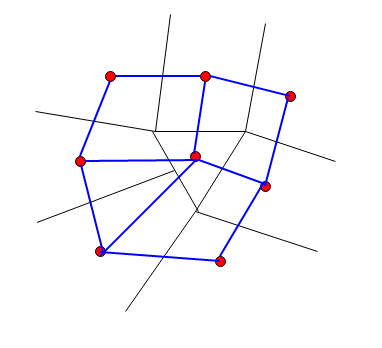
\includegraphics[width= \textwidth]{images/voronoiandDelanauy.png}
      		\caption{}
      		\label{VoronoiDelaunay}
      	\end{subfigure}
      	\caption{A sample Vorronoi diagram on $8$ seeds/points (red) (\subref{VoronnoiDiag}) and its corresponding dual graph (Delaunay Triangulation in blue) superimposed (\subref{VoronoiDelaunay}).}
       \end{figure}
  
      
      
     Corner point detection, Voronoi diagrams, and Delaunay triangulation are very useful methods in the extraction of graphs from objects. In later chapters of this work, we demonstrate the process of image extraction from objects of selected database using a combination of the $3$ mentioned concepts.
     
     \subsection{Graph embedding}
     In this era where graphs manifest in a number of fields ranging from chemistry, infrastructure, social and biology,  there is quite large amounts of data represented in graph form from which information needs to be extracted. \\
     
     Graph analysis for purposes of obtaining useful information has been greatly explored by researchers recently and various techniques have been put forward to attaining this task. It is worth noting that effective graph analysis can aid in classification of nodes/graphs, link predictions, graph visualisations, graph clustering among others.
     One efficient and effective way of handling the task of graph analysis is graph embedding. Graph embedding is a way of mapping a graph into a low-dimensional vector space in which all graph information is preserved. Such information includes structural information, node label or attribute information, among others. 
     The task of graph embedding involves an input as well as an output. The embedding input is normally a graph which could be homogeneous, heterogeneous, attributed graph or graph constructed from relational data. Given an input graph, different embedding outputs can be obtained depending on the task at hand. The outputs include node embedding, edge embedding, substructure embedding and whole-graph embedding. In this work, however, we will consider whole-graph embedding where a whole-graph is represented as a vector.  Formally, we consider mapping of a set of graphs to vectorial space, that is,
     
     \begin{equation}
     \Phi : G \longrightarrow \mathbb{R}^n, \quad 
     g \longrightarrow \Phi(g) = (f_1, f_2, f_3, \cdots, f_n)
     \end{equation}     
     
     There are various methods studied in literature that are used in creating feature vectors of graphs. These can be categorised as spectral clustering methods, Substructure finding methods, and Dissimilarity representation. For purposes of this work, we explore the spectral clustering methods and related invariants in Chapter. 
     
     \subsection{Principal Component Analysis (PCA)}
	  Principal Component Analysis is a very important and widely used statistical technique in various applications such as image compression, face recognition, pattern identification in high dimensional data, among others. It is such a powerful tool for data analysis especially for dimension reduction of data \citep{shlens2014tutorial}. Before we dive into details of PCA, let us first define some of the statistical concepts that we will come across most often. Given a sample of size $n$ of a population. We have the following definitions in \citep{smith2002tutorial} :\\
	  
	  \begin{defn}[Mean]
	  	The mean, $\bar{X}$, of a sample is the average of elements of the sample and is given by
	  	\begin{equation}
	  	\bar{X} = \frac{\sum_{i=1}^{n} X_i}{n}
	  	\end{equation}
	  \end{defn}
    
      \begin{defn}[Standard Deviation]
      	The standard deviation of a data set is a measure of how spread out the data is. It is average distance of a given point from the mean of the data set. The standard deviation, denoted by $\sigma$ is given by
      	\begin{equation}
      	\sigma = \sqrt{\frac{\sum_{i=1}^{n} (X_i - \bar{X})^2}{(n-1)}}
      	\end{equation}
      \end{defn}
  
      \begin{defn}[Variance]
      	The variance, $\sigma^2$, is the square of the standard deviation. It is also a measure of spread of a data set. It is given by
      	\begin{equation}
      	\sigma^2 =  \frac{\sum_{i=1}^{n} (X_i - \bar{X})^2}{(n-1)}
      	\end{equation}
      	It is important to note that both the standard deviation and variance measure the spread of a data set that is $1$-dimensional. \\
      \end{defn}
  
      \begin{defn}[Covariance]
      	For data sets with more than $1$ dimension, we use the covariance instead of variance (or standard deviation) to measure the deviation from the mean amongst any pair of dimensions. The covariance of two dimensions $x$ and $y$ is given by
      	\begin{equation}
      	cov(X,Y) = \frac{\sum_{i=1}^{n} (X_i - \bar{X}) (Y_i - \bar{Y})}{(n-1)}
      	\end{equation}\\
      \end{defn}
  
       \begin{defn}[Covariance matrix]
       	For a set of data with $n$ dimensions, the covariance matrix is given by
       	\begin{equation}
       	C^{n \times n} = (c_{i,j}, c_{i,j} = cov(Dim_i, Dim_j)),
       	\end{equation}
       	where $C^{n \times n}$ is a matrix with $n$ rows and $n$ columns, $Dim_i$ is the $i$th dimension. 
       \end{defn}
       For example, for a data set with $3$ dimensions $x$,$y$, and $z$, we write the covariance matrix as
       \begin{equation}
       C = \begin{pmatrix}
       cov(x,x) & cov(x,y) & cov(x,z) \\
       cov(y,x) & cov(y,y) & cov(y,z) \\
       cov(z,x) & cov(z,y) & cov(z,z)
       \end{pmatrix}
       \end{equation}
       
       Given a set of data with $n$ dimensions, we perform PCA on the data set following the steps below:
       \begin{itemize}
       	\item Compute the mean for each dimension and then subtract the mean from the respective dimension for instance for dimensions $x$ and $y$, subtract each $x$ value, compute $x-\bar{x}$ and for each $y$ value, compute $y-\bar{y}$. The data obtained after subtracting the mean is referred to as Normalised data.
       	\item Calculate the covariance matrix as explained previously.
       	\item Compute the eigenvalues and eigenvectors of the covariance matrix.
       	\item For dimensional reduction and data compression, choose principal components which are the eigenvectors corresponding to largest eigenvalues. The principal components are the directions where there is most variance (that is, where data is most spread).
       	The number of principal components corresponds to the new dimensionality.
       	\item Feature vector formation. Having chosen which eigenvectors to keep, we construct the feature vector which is a matrix with the chosen eigenvectors as columns.
       	\item New data set. We obtain the new data set (with reduced dimensions) by 
       	 \begin{equation}
       	 NewData = FeatureVector^T \times NormalisedData^T
       	 \end{equation}
       	
       \end{itemize}
       Having obtained the feature vectors as explained in the previous subsection, we create a database whose columns are the feature vectors for each graph. We can then apply principal components analysis to the database so as to embed the respective graphs onto low dimension space as we will elaborate in the following chapters.
     
    \newpage
    \section{Diffusion on networks}
    Dynamical processes on networks aid in the modelling of processes that occur in real-world systems for example spread of diseases in a social group, transmission of signals in brain networks, spread of information in a social network, and many others. In this work, we explore the diffusion process is one of the most popular dynamic processes studied in literature.
    
    According to \citep{newman2010networks}, diffusion is, among others, the movement of substance from a region of high concentration to a region of low concentration. Such substance include heat, gas, and many more. 
    The diffusion process on networks is used in developing models that depict processes that occur in real-world systems. The modeling scheme used in this case involves: First, identifying each node of a network with a particular component or part of the system. Secondly, for each node $i$, a variable $\sigma_i$ is introduced that characterises its dynamical state \citep{barrat2008dynamical}. Examples of diffusion models that adopt the mentioned modeling scheme can be found in \citep{estrada2011epidemic,kasprzak2012diffusion,lopez2008diffusion}. 
    
    In this work, we discuss the diffusion of heat on a network in which we explore the diffusion model where diffusion occurs only along edges of a network, study the equilibrium behaviour of this model and also ascertain the impact of structure,  selection of source nodes, and  network homogeneity on rate of diffusion on a network through simulations. We also explore diffusion on directed networks and discuss equilibrium behaviour on different types of directed networks.
    
    Furthermore, we consider another diffusion model that involves both direct interactions ( among nearest neighbor nodes) as well as long-range interactions among non-nearest nodes in the network. We explore this model as  many processes in real-world involve some kind of long-range interaction for example epidermic spread in population, synchronisation processes in physics, consensus problems, to mention but a few.
    In accounting the long-range interactions, we adopt a method put forward by Estrada in \citep{estrada2012path,estrada2017long}.
    
    
    \subsection{Heat diffusion model}
    Recently, various models have been developed to depict the process of heat diffusion on networks. Here, we consider a simple model on a simple graph as explained:
    
%    which include selection of marketing candidates in social network marketing, data analysis and processing in which the observed data is considered as a sum of diffusion processes, dimensionality reduction and classification problems   \citep{ma2008mining,thanou2017learning,belkin2003laplacian}.
    
    Let $G=(V,E)$ be a simple connected undirected graph with vertex set $V$ and edge set $E$. Suppose we randomly select a few nodes ( that is, sources) to which we assign specific amounts of heat as in vector $\phi_0$. Let $\varepsilon \in [0,1]$ be the heat diffusion coefficient that controls the rate of diffusion. When $\varepsilon$ tends to $0$, heat transfer among nodes becomes difficult and as a result, heat does not spread to each of the nodes with in the network. However, as $\varepsilon$ tends to $1$, heat spreads rapidly among nodes and thus, with out loss, heat is distributed to all nodes in the network.
    
   At each time $t$, we obtain the quantities, $\phi_i(t)$, of heat at each node, $i$. The spread of heat is considered to occur along the edges connecting nodes, that is to say, through direct interactions.  
%     We then try to understand how the heat will spread through out the network, whether equilibrium can be attained and if so, when does this happens?? We then explore the impact of network structure and node centralities on heat diffusion.
%    \begin{enumerate}[a)]
%    	\item Direct interactions
%    	Let us consider a simple network where a few randomly selected nodes are assigned quantities of heat $\phi_i$. The diffusion process is considered to occur by means of interactions between neighbouring nodes in the network. This mode of interaction is referred to as direct interactions. 
    	
    	The process of heat spread through out the network can therefore be modelled by
    	\begin{equation}
    	\frac{d\phi_i(t)}{dt} = \varepsilon \sum_j (\mathbf{A}_{ij} - \delta_{ij} k_i) \phi_j(t),
    	\label{difusion}
    	\end{equation}
    	where $\mathbf{A}$ is the adjacency matrix, $k_i$ is the degree of node $i$, and $\delta_{ij}$ is the Kronecker delta whose value is $1$ if $i=j$ and $0$ otherwise. In matrix-vector notation, we have
    	\begin{equation}
    	\frac{d\boldsymbol{\phi}(t)}{dt} = -\varepsilon\mathbf{L}\boldsymbol{\phi}(t), \quad \boldsymbol{\phi}(0) = \boldsymbol{\phi}_0 ,
    	\label{dif-final-eqn}
    	\end{equation}
    	where $\mathbf{L}$ is the Laplacian matrix of a graph. Alternatively, the normalised version $\mathcal{L}$ of the Laplacian is used.
    	\begin{rem} 
    		It is worth noting that for diffusion processes, the normal Laplacian $\mathbf{L}$ performs well as is its normalised counterpart. Thus, for most simulations of diffusion in this work, we use the normal Laplacian matrix.
    	\end{rem}
    	The solution to equation \ref{dif-final-eqn} is 
    	\begin{eqnarray}
    	\boldsymbol{\phi}(t) = \boldsymbol{\phi}_0~e^{-\varepsilon t \mathbf{L}}.
    	\end{eqnarray}
    	Alternatively, the solution can be expressed as a linear combination of eigenvectors of the Laplacian matrix. That is
    	 \begin{eqnarray*}
    	 	\boldsymbol{\phi}(t) = \sum_i \langle \boldsymbol{\phi}(0),\mathbf{v}_i \rangle \quad e^{-\varepsilon\lambda_i t} \mathbf{v}_i,  
    	 \end{eqnarray*}
    	 where $\lambda_i$, $\mathbf{v}_i$ are respectively the eigenvalues and corresponding eigenvectors of the Laplacian matrix and $\langle \boldsymbol{\phi}(0),\mathbf{v}_i \rangle$ is simply the projection of $\boldsymbol{\phi}(0)$ onto the set of eigenvectors \citep{anton2007elementary}.
    	 
    	 \subsection{ Equilibrium behaviour }
    	 We study the behaviour of the diffusion process and the quantities of heat at each of the nodes after an infinite period of time. 
    	 For a simple undirected network, as $t$ goes to infinity, we have 
    	 \begin{equation}
    	 \lim_{t \to \infty} e^{-\varepsilon\lambda_i t} = \begin{cases} 0 &\mbox{if } \lambda_i > 0 \\
    	 1 & \mbox{if } \lambda_i = 0, \end{cases} 
    	 \end{equation}
    	 Asymptotically, the equilibrium state is completely determined by the kernel of $\mathbf{L}$. Since $\sum_{j} \mathbf{L}_{ij}=0$, it is easy to see that $\mathbf{v^1}= \frac{1}{\sqrt{n}}[1,\cdots,1]$, the eigenvector associated with $\lambda_i =0$, is in the kernel of $\mathbf{L}$. We then have
    	 %$\displaystyle \lim_{t \to \infty}\boldsymbol{\phi}(t)$, $a_i(t) = a_i(0) e^{-C \lambda_i t}$ where $\lambda_i = 0$. Since $L(\mathbf{v^1}) = \mathbf{0}$, for a given initial condition $\mathbf{a}(0)$ for a network with $n$ nodes, we have
    	 \begin{equation}
    	 \lim_{t \to \infty}\boldsymbol{\phi}(t) = \langle \boldsymbol{\phi}(0), \mathbf{v^1} \rangle \mathbf{v^1}.
    	 \end{equation}
    	 The quantity of heat $\phi_j(t)$ at any node $j$ at time $t$ is given by
    	 \begin{equation}
    	 \lim_{t \to \infty}\phi_j(t) = \frac{1}{n} \sum_{i = 1}^n \phi_i(0). 
    	 \end{equation}
    	 At steady state, the quantity $\phi_i(t)$ at each of the nodes is the same, which is the average of the initial values at all of nodes. This is because, as expected, neighboring nodes in the network will exchange heat amongst each other until all nodes attain equal amounts of heat (i.e no difference in amount for any given pair of nodes).
    	 
    	 For better understanding of the heat diffusion model, let us consider the following simple example.
    	 
    	 \begin{exa} Let us consider diffusion of heat over the network in Fig.~\ref{graph-plot}(\subref{difn-graph}). Suppose the quantity of heat at each node at time $t=0$ is given by the vector $\boldsymbol{\phi}(0)= [0.3,0.0,0.8,0.0,0.5,0.2,0.0,0.0,0.0,0.2]$, random values between $0$ and $1$. Let $\varepsilon=0.05$. Fig.~\ref{graph-plot}(\subref{difn-plot}) illustrates how heat spreads over the network in Fig.~\ref{graph-plot}(\subref{difn-graph}). 
    	 	
    	 	\begin{figure}[H]
    	 		\centering
    	 		\begin{subfigure}[b]{0.29\textwidth}
    	 			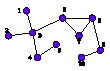
\includegraphics[width=\textwidth]{images/diffusion-graph.pdf}
    	 			\caption{}
    	 			\label{difn-graph}
    	 		\end{subfigure}~
    	 		\begin{subfigure}[b]{0.45\textwidth}
    	 			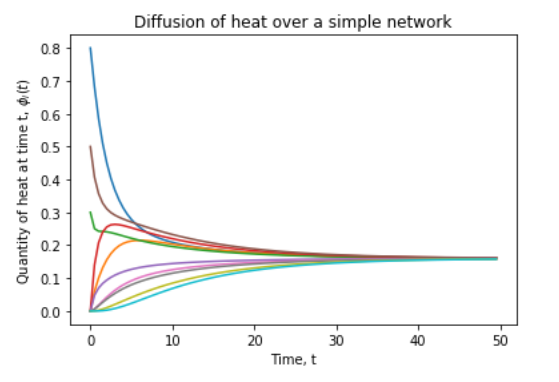
\includegraphics[width= \textwidth]{images/Diffusion-on-network-new.png}
    	 			\caption{}
    	 			\label{difn-plot}
    	 		\end{subfigure}
    	 		\caption{ Results from simulation of diffusion process over the network in (\subref{difn-plot}). }
    	 		\label{graph-plot}
    	 	\end{figure}
     	  From Fig.\ref{graph-plot}, we observe that at each time step $t$, nodes that initially have high amounts of heat (i.e $1,3,5,6,$ and $10$) exchange heat with adjacent nodes that initially had none or little amounts of heat. The latter gain heat from the former and eventually all nodes in the network have relatively equal amounts of heat. This explains the fact that as time $t$ increases, the quantity of heat $\boldsymbol{\phi}_j(t)$ at each node tends to the equilibrium value of $0.2$ which is attained as $t$ approaches $50$. 
    	 \end{exa}
     
     \subsection{Impact of network structure on the rate of diffusion}
     The structure of a network basically means the way in which nodes are connected in the network. For instance, in a regular network each node is connected to equal number of nodes, for a star network one node is positioned in a way that all other nodes are connected to it. Since diffusion on networks occurs due to the interactions within neighbourhoods of nodes, it therefore implies that the topology of a network has a strong influence on the diffusion process. 
     
     We consider two networks with different structures: one is an Erdos-Renyi (ER) network that follows a Poisson degree distribution and the other
     Barabasi-Albert (BA) network in which connection of nodes follows scale free power-law distribution, that is to say, the probability of finding a node with degree $k$ decreases as the negative power of $k$. We perform simulations of diffusion on these networks and the results are explained:
%     in which a pair of nodes is connected by random probability, $p$. The degree of nodes in ER network follow a Poisson distribution \cite{erdos1960evolution}. Second, we consider the Barabasi-Albert(BA) network in which connection of nodes follows scale free power-law distribution, that is to say, the probability of finding a node with degree $k$ decreases as the negative power of $k$. It therefore less likely to find a node with high degree (hub) compared to low degrees \cite{barabasi1999emergence, estrada2011structure} . 
     Consider ER and BA networks with $n=100$ and average degree $\bar{k}= 2.3$, we randomly select $20$ nodes to which we assign random quantities (range of 0 to 20) of heat and then allow diffusion to occur. After every time step $t$, we compute the quantities at each node as depicted in Figure \ref{barabasi-Erdos-compare}.
     \begin{figure}[H]
     	\centering
     	\begin{subfigure}[b]{0.45\textwidth}
     		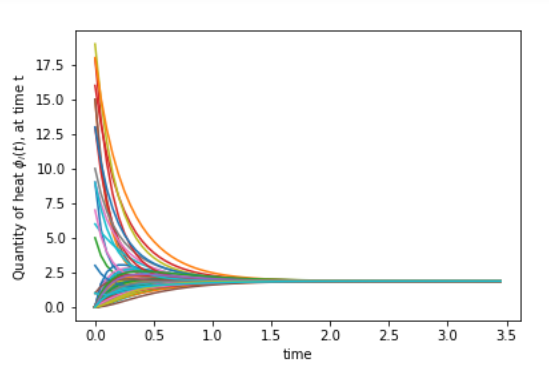
\includegraphics[width=\textwidth]{images/Barabasi-normalDiffusion.png}
     		\caption{}
     		\label{barabasi-normal}
     	\end{subfigure}~
     	\begin{subfigure}[b]{0.45\textwidth}
     		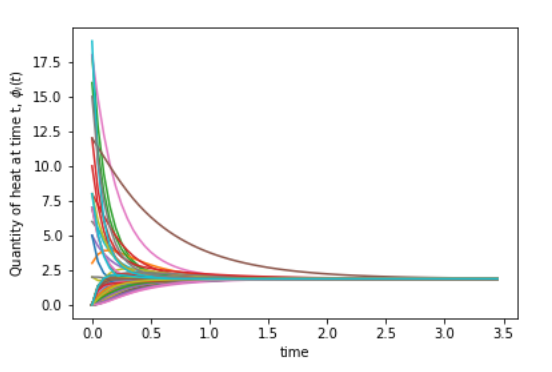
\includegraphics[width= \textwidth]{images/E-R-normalDiffusion.png}
     		\caption{}
     		\label{ER-normal}
     	\end{subfigure}
        \caption{Simulations for diffusion on networks following equation \ref{dif-final-eqn}. To the left is the BA network and to the right is ER. Both networks have $100$ nodes and average path length $2.3$. }
     	\label{barabasi-Erdos-compare}
     \end{figure}
      From Fig \ref{barabasi-Erdos-compare} we observe that diffusion occurs much faster in BA network than in ER network. In BA, equilibrium is reached after $1.5$ time steps while in ER network equilibrium is reached much later after $2.5$ time steps. This behaviour is attributed to the different structures of the two networks. The BA network is composed of highly connected nodes known as hubs that interact with a number of nodes at the same time thus fastening the diffusion process. On the other hand, the ER network is homogeneous which means there are no hubs and for that reason, diffusion occurs quite slower than in BA networks as evident in Fig.~\ref{barabasi-Erdos-compare}. Following these results, we can see that the structure of a network plays a key role in influencing the rate of diffusion and thus a determinant of how fast equilibrium is attained.
      
     %\newpage
%     \begin{figure}[H]
%     	\centering
%     	\begin{subfigure}[b]{0.45\textwidth}
%     		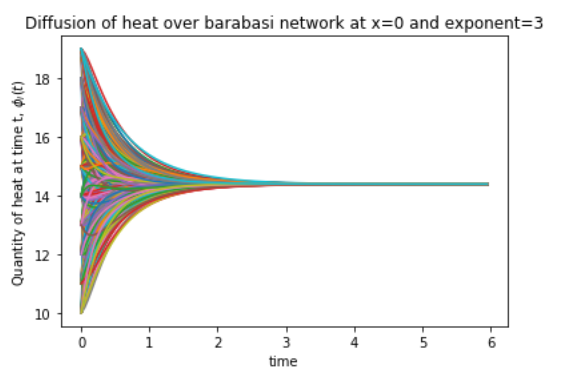
\includegraphics[width=\textwidth]{images/barabasi-x0.png}
%     		\caption{$x=0$}
%     		\label{barabasi-x0}
%     	\end{subfigure}~
%     	\begin{subfigure}[b]{0.45\textwidth}
%     		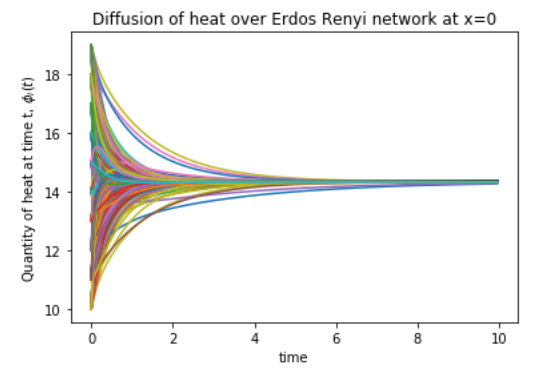
\includegraphics[width= \textwidth]{images/erdos-x0.png}
%     		\caption{$x=0$}
%     		\label{erdos-x01}
%     	\end{subfigure}\\
%     	\begin{subfigure}[b]{0.45\textwidth}
%     		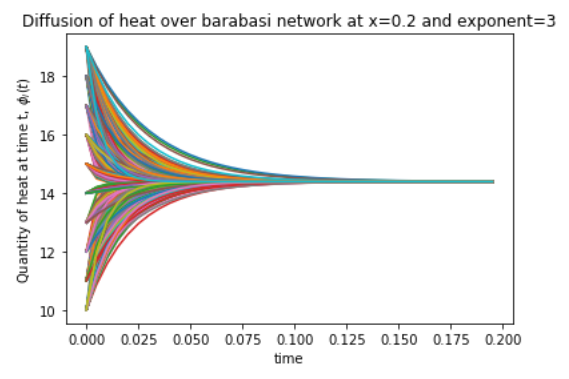
\includegraphics[width= \textwidth]{images/barabasi-x02.png}
%     		\caption{$x=0.2$}
%     		\label{barabasi-x02}
%     	\end{subfigure}~
%     	\begin{subfigure}[b]{0.45\textwidth}
%     		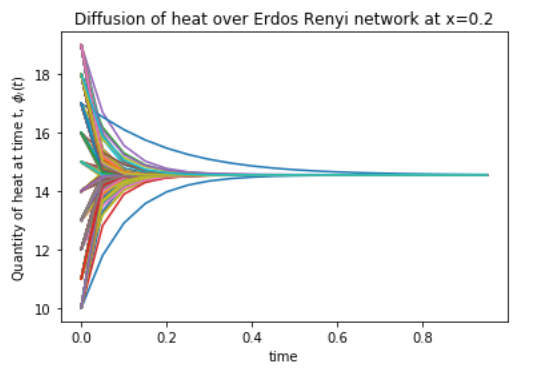
\includegraphics[width= \textwidth]{images/erdos-x02.png}
%     		\caption{$x=0.2$}
%     		\label{erdos-x02}
%     	\end{subfigure}\\
%     	\begin{subfigure}[b]{0.45\textwidth}
%     		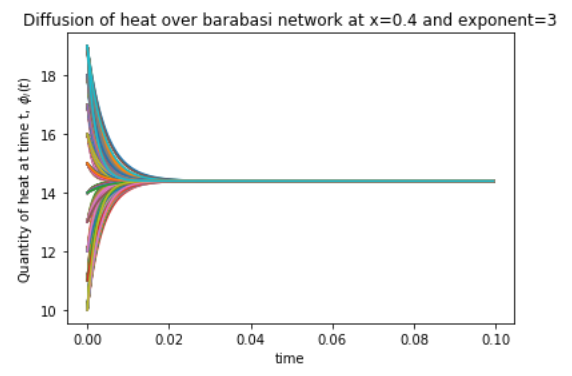
\includegraphics[width= \textwidth]{images/barabasi-x04.png}
%     		\caption{$x=0.4$}
%     		\label{barabasi-x04}
%     	\end{subfigure}~
%     	\begin{subfigure}[b]{0.45\textwidth}
%     		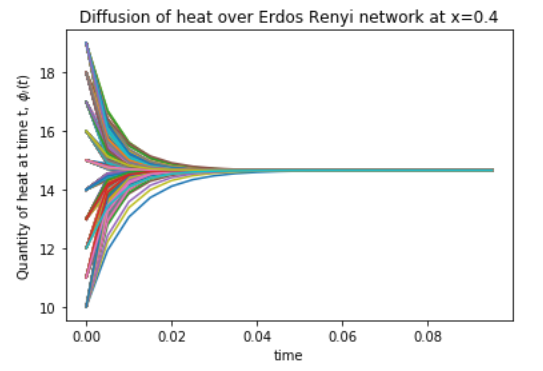
\includegraphics[width= \textwidth]{images/erdos-x04.png}
%     		\caption{$x=0.4$}
%     		\label{erdos-x04}
%     	\end{subfigure}
%     	\caption{Barabasi networks (left) and Erdos Renyi networks(right) of 1000 nodes and average degree of 6. Top row is illustration of diffusion process at $x=0$ ( i.e accounting for direct interactions only), middle row corresponds to $x=0.2$ followed by $x=0.4$ in the last row}
%     	\label{barabasi-Erdos-compare}
%     \end{figure}
%     
%     From Fig \ref{barabasi-Erdos-compare} at the top row, we observe that at $x=0$, equilibrium is reached faster for Barabasi-Alberto(BA) network ( that is after about $4$ time steps) compared to Erdos-Renyi(ER) network in which equilibrium is reached after about $10$ time steps. This is explained based on the fact that in BA networks there are more hubs compared to ER networks. These hubs tend to interact with a number of nodes with in the network thus fastening the diffusion process. On increasing $x$ to $0.2$, we observe a drastic drop in equilibrium time from  $4$ to $0.15$ time steps and from $10$ to $0.8$ time steps for BA and ER networks respectively. It is important to note that drop in equilibrium time is relatively higher in ER than in BA and this is because of the few hubs in ER networks which aids a larger number of long range interactions than in BA networks. As $x$ increases further to $0.4$, equilibrium time further drops to $0.03$ and $0.06$ for BA and ER networks respectively.
     
     \subsection{Influence of heterogeneity on diffusion over network}
     
     Here, we consider heterogeneity in scale free networks with total number of nodes $n=1000$ and average degree $\bar{k}=20$ by varying power exponent, $\gamma$. For different conductances $x$, we assign initial quantities of heat to each of the $200$ nodes with highest degree. Figure \ref{quantity-exponents} illustrates how the average quantities of heat of the selected initial diffusion nodes varies with time.
     \begin{figure}[H]
     	\centering
     	\begin{subfigure}[b]{0.35\textwidth}
     		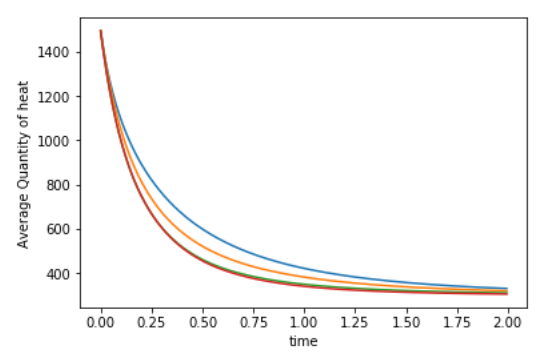
\includegraphics[width=\textwidth]{images/quantity-time-exponents-x0.png}
     		%\caption{$x=0.1, t=0$}
     		%\label{gridt0x01}
     	\end{subfigure}~
     	\begin{subfigure}[b]{0.35\textwidth}
     		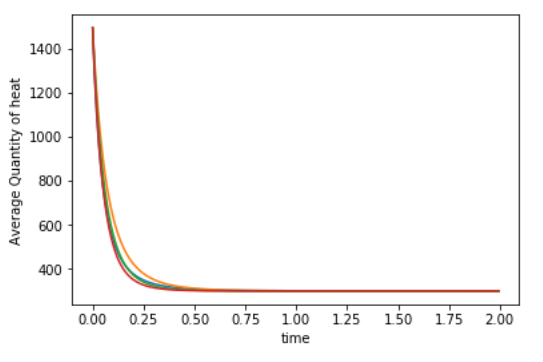
\includegraphics[width= \textwidth]{images/quantity-time-exponents-x01.png}
     		%\caption{$x=0.1, t=0.5$}
     		%\label{gridt05x01}
     	\end{subfigure}\\
%     	\begin{subfigure}[b]{0.35\textwidth}
%     		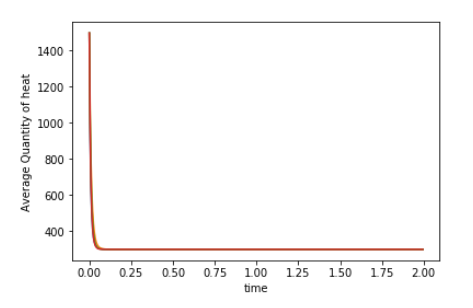
\includegraphics[width= \textwidth]{images/quantity-time-exponents-x03.png}
%     		%\caption{$x=0.1, t=3.0$}
%     		%\label{gridt3x01}
%     	\end{subfigure} \\
     	\begin{subfigure}[b]{0.80\textwidth}
     		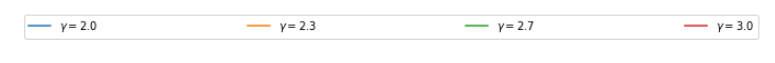
\includegraphics[width= \textwidth]{images/legend-gamma.png}
     	\end{subfigure}
     	\caption{Plots of the average quantity of heat for $200$ nodes with the highest degree centrality against time for $3$ scale free networks having different values of the power exponent($2.0$,$2.3$,$2.7$, and $3.0$), n=1000 and average degree=$6$. The figures to the left, centre and right correspond to x values $0$, $0.1$, and $0.3$ respectively.}
     	\label{quantity-exponents}
     \end{figure}
 
     \subsection{Impact of choice of initial diffusion nodes on the diffusion process on networks}
     We consider a BA network and ER network, both of $100$ nodes and average path length of $6$. First case, we select $20$ nodes in both networks with the highest degree centrality to which we assign specific amounts of heat. Second case, we randomly select $5$ nodes in both networks. At each time $t$, we measure the average quantity of heat at the $20$ nodes and the results of the simulations are illustrated by Fig.~\ref{sourceimpact}.
     
     \begin{figure}[H]
     	\centering
     	\begin{subfigure}[b]{0.45\textwidth}
     		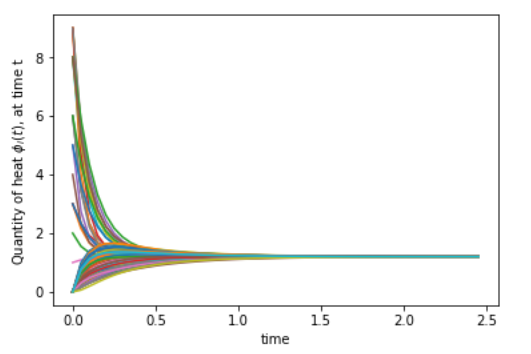
\includegraphics[width= \textwidth]{images/BA-degreesource.png}
     		\caption{}
     		\label{}
     	\end{subfigure}~
     	\begin{subfigure}[b]{0.45\textwidth}
     		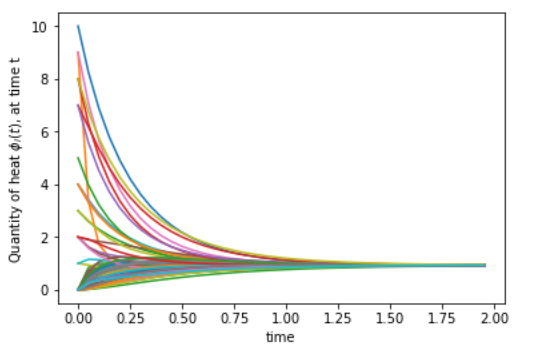
\includegraphics[width= \textwidth]{images/BA-randomsource.png}
     		\caption{}
     		\label{}
     	\end{subfigure}\\
     	\begin{subfigure}[b]{0.45\textwidth}
     		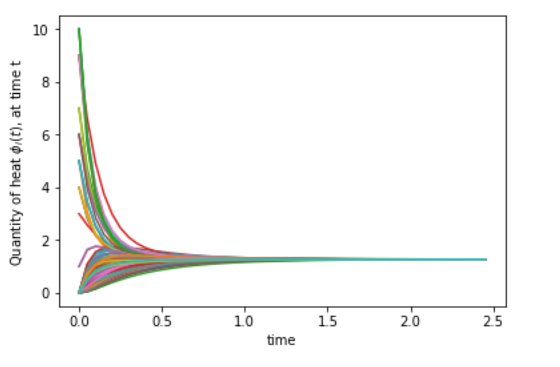
\includegraphics[width= \textwidth]{images/ER-degreesource.png}
     		\caption{}
     		\label{}
     	\end{subfigure}~
     	\begin{subfigure}[b]{0.45\textwidth}
     		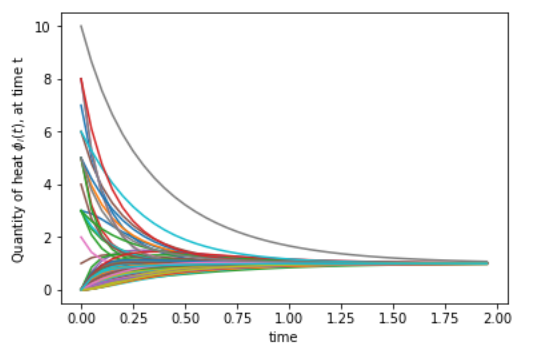
\includegraphics[width= \textwidth]{images/ER-randomsource.png}
     		\caption{}
     		\label{}
     	\end{subfigure}
     	\caption{ Results of the simulations for two networks. The top row corresponds to the BA network, (left) is illustration for which the $20$ source nodes are ones with the highest degree and (right) is illustration for randomly selected source nodes. On the other hand, the bottom row is ER network for which (left) corresponds to diffusion for which the source nodes are the highest degree nodes and the figure to the right is one for which the source nodes are selected randomly.}
     	\label{sourceimpact}
     \end{figure}
     
     From the simulations, we observe that when the source nodes (those  from which diffusion commerces) are chosen based on the degree, diffusion occurs much faster and equilibrium is attained quickly compared to when the source nodes are chosen randomly. We explain this observation based on the fact when the highest degree nodes initiate the diffusion process, they quickly interact with their neigbouring nodes at the same time and since their neighbourhood is big in size, this results into fast spread of heat among the nodes in the network. On the other hand, when source nodes are randomly selected, their is a possibility of including nodes with low degree among the selection, these low degree nodes are not fast agents of heat transfer due to their small neighbourhood which results into a relatively slow diffusion process.
     
     \newpage
     
        \subsection{Diffusion on directed networks}
        A directed graph, also known as a digraph or directed network, is one in which all the edges are directed from one vertex to another. 
        
        There are various complex systems whose structural skeleton can be captured by directed networks. Examples include ecological  networks, power grids, transportation networks, communication networks, metabolic networks, gene regulatory networks, citation networks among others. It is therefore paramount to study how dynamic processes such as diffusion, consensus, occur on such networks. There are various categories of directed networks which include:\\
        
        \begin{defn}[Weakly connected digraph]
        	A directed graph is called weakly connected if replacing all of its directed edges with undirected edges produces a connected (undirected) graph.\\
          \end{defn}   
        \begin{defn}[Strongly connected digraph]
        	A digraph is called strongly connected if and only if any two distinct nodes of the graph can be connected via a path that respects the orientation of the edges of the digraph \citep{saber2003agreement}.\\
        \end{defn}        
        For a strongly connected digraph with atleast two distinct nodes and with no self loops, the diffusion process on this network can be modelled in a similar manner as its undirected counterpart by 
        \begin{equation}
        \frac{d\boldsymbol{\phi}}{dt} = -\varepsilon\mathbf{L}\boldsymbol{\phi}, \quad \boldsymbol{\phi}(0) = \boldsymbol{\phi}_0.
        \end{equation}
        For undirected graph $G$, the graph Laplacian  $\mathbf{L}$, is symmetric positive semi-definite. However, for directed graphs $\mathbf{L}$ is non-symmetric which implies that the diffusion on the former and latter graphs is not necessarily the same.\\
        
         \begin{defn}[Balanced Graphs]
        	We say the node $v_i$ of a digraph $G=(V,E)$ is balanced if and only if its in-degree and out-degree are equal, that is, $d_{out}(v_i) =d_{in}(v_i)$. A graph $G$ is balanced if and only if all its nodes are balanced, i.e $\sum_j a_{ij} = \sum_j a_{ji}, \forall i$. 
        \end{defn}
        
        \subsection{Equilibrium behaviour in directed network}
        In order to understand the process of attainment of steady state in networks, we need to study the spectral properties of graph Laplacian. Let $G=(V,E)$ be a digraph with Laplacian $\mathbf{L}$ with eigenvalues $\lambda_1, \lambda_2, \cdots, \lambda_n$ in non-decreasing order. 
        \subsubsection{Estimation of eigenvalues of the Laplacian}
        Let $d_{max}$ be the maximum node out-degree of $G$, then following from Gershgorin disk theorem, then all the eigenvalues of $\mathbf{L}$ are located in the following disk
        \begin{equation} 
        \mathbf{D} = \{ z \in \mathbb{C} : |z-d_{max}| \leq d_{max} \}
        \end{equation}
        with centre at $z = d_{max} +0j$ in the complex plane \citep{saber2003agreement}. Thus, for a strongly connected digraph $G$, $\mathbf{L}$ has a zero eigenvalue $\lambda_1=0$ and all the other non-trivial eigenvalues have non-negative real parts.
        Let us consider a strongly connected digraph $G=(V,E)$. Let $\boldsymbol{\phi}_0$ be the vector of quantities of heat at all nodes at $t=0$, $\varepsilon=1$ be the diffusion coefficient. Similar to undirected case,the quantities of heat, $\boldsymbol{\phi}(t)$ at each node at a given time $t$ is given by
        \begin{equation}
        \boldsymbol{\phi}(t) = \boldsymbol{\phi}_0~e^{-\mathbf{L}t}.
        \end{equation}
        
        \begin{thm}[Limit Theorem for Exponential Matrices]
        	Assume $G$ is a strongly connected digraph with Laplacian $\mathbf{L}$ satisfying $\mathbf{L} \mathbf{v}_r = \mathbf{0}$, $\mathbf{v}_{l} ^T \mathbf{L} =\mathbf{0}$, and $\mathbf{v}_{l} ^T \mathbf{v}_r=1$. Then 
        	
        	\begin{equation}
        	 R = \lim_{t \longrightarrow +\infty} e^{(-\mathbf{L}t)
        	} = \mathbf{v}_r  \mathbf{v}_{l} ^T \in M_n,
        	\end{equation}
        	where $M_n$ denotes a set of square $n\times n$ matrices, $\mathbf{v}_r$,and $\mathbf{v}_{l} ^T$ denote the right and left eigenvalues of $\mathbf{L}$ associated with eigenvalue $\lambda_1 = 0$ \citep{saber2003agreement}.
        	\label{exponentialTheorem}
        \end{thm}
    From the theorem, we deduce that for a strongly connected digraph, equilibrium state can be attained and the quantity of heat at the nodes is given by
    \begin{equation}
    \lim_{t \longrightarrow \infty} =  \boldsymbol{\phi}_0  \mathbf{v}_r  \mathbf{v}_{l} ^T
    \label{equildirected}
    \end{equation}
    It is important to note that following Equation \ref{equildirected}, any equilibrium value $x^*$ can be attained such that $x^*_i =x^*_j$ for all $i$, $j$. This therefore motivates the search for which classes of digraphs attain equilibrium similar to that of undirected graphs where the value at each node is the average of the initial values at all nodes in the network.
    
    \begin{prop}
    Consider a directed network $G=(V,E)$ that is strongly connected. Then the digraph $G$ globally attains average equilibrium if and only if $\mathbf{1}^T \mathbf{L}= \mathbf{0}$ \citep{saber2003agreement}.
    \label{prop1}
    \end{prop} 

    \subsubsection{Equilibrium state for balanced graphs}
     The proposition in \citep{saber2003agreement} states that \\
     
     \begin{prop}
     Let $G=(V,E)$ be a digraph with an adjacency matrix $A=[a_{ij}]$ satisfying $a_{ii}=0, \forall i$. Then, all the following statements are equivalent:
     \begin{enumerate}[i)]
     	\item $G$ is balanced,
     	\item $\mathbf{v}_l = \mathbf{1}$ is the left eigenvector of the Laplacian of $G$ associated with the zero eigenvalue, that is, $\mathbf{1}^T \mathbf{L} = 0$.
     	\item $\sum_{i=1} ^ n u_i = 0, \forall x \in  \mathbb{R}^n$ with $u_i = \sum_{j \in N_i} a_{i,j} (x_j -x_i).$
     \end{enumerate}
     \label{prop1}
     \end{prop}
 
      Since for a balanced digraph $\mathbf{v_l}$ is an all ones vector, it therefore follows from Proposition \ref{prop1} that at equilibrium, the value at all nodes in a balanced graph is the average of the initial values at all nodes. \\
      
      \begin{exa}
      	Let us consider two directed graphs, one is a balanced digraph and the other is not. We then assign initial quantities of heat to all nodes in the order $0$ to $4$ as in the vector $\phi_0=[2,0,3,0,0]$ and set the diffusion coefficient, $C=1$. We then obtain plots for diffusion on both graphs after a specific time $t$ as shown in Figs.~ \ref{unbalanced-diffusion}(\subref{plot-balanced}) and \ref{unbalanced-diffusion}(\subref{plot-unbalanced}).
      	
      	\begin{figure}[H]
      		\centering
      	    \begin{subfigure}[b]{0.40\textwidth}
      	    	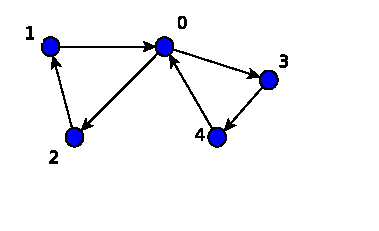
\includegraphics[width=\textwidth]{images/balanceDigraph.pdf}
      	    	\caption{}
      	    	\label{balanced-graph}
      	    \end{subfigure}~
      	    \begin{subfigure}[b]{0.5\textwidth}
      	    	\includegraphics[width= \textwidth]{images/Balanced-digraph-diffusion.png}
      	    	\caption{}
      	    	\label{plot-balanced}
      	    \end{subfigure} \\
            \begin{subfigure}[b]{0.40\textwidth}
            	\includegraphics[width=\textwidth]{images/UnbalanceDigraph.pdf}
            	\caption{}
            	\label{unbalanced-graph}
            \end{subfigure}~
            \begin{subfigure}[b]{0.5\textwidth}
            	\includegraphics[width= \textwidth]{images/non-balnceddigraph-difusion.png}
            	\caption{}
            	\label{plot-unbalanced}
            \end{subfigure}
      		\caption{Diffusion over different categories of directed networks. (\subref{unbalanced-graph}) is an illustration of diffusion over weakly connected and unbalanced digraph in (\subref{balanced-graph}). (\subref{unbalanced-graph}) is an illustration of diffusion over strongly connected and balanced digraph (\subref{unbalanced-graph}).  }  
      		\label{unbalanced-diffusion}		
      	\end{figure} 
   For the balanced graph in Fig.~\ref{balanced-graph}, its Laplacian matrix $\mathbf{L}$,$v_r$ and $v_l$ are respectively:
   \begin{equation*}
   \mathbf{L} = \begin{pmatrix}
    2 &  0 & -1 & -1 &  0 \\
   -1 & 1  & 0  & 0  &  0 \\ 
    0 & -1 & 1  & 0  &  0 \\
    0 &  0 & 0  & 1  & -1 \\
    -1&  0 & 0  & 0  & 1
   \end{pmatrix}, \quad 
   v_r = v_l = \begin{pmatrix}
   0.4472136 \\  
   0.4472136 \\  
   0.4472136 \\ 
   0.4472136 \\
   0.4472136
   \end{pmatrix}
   \end{equation*} 
   The values for $v_r$ and $v_l$ satisfy Theorem \ref{exponentialTheorem} as well as Proposition \ref{prop1} and thus, equilibrium is attained at $x^*=1.0$ which is the average of initial values $x_0$.\\
   On the other hand, for the unbalanced graph in Fig.~\ref{unbalanced-graph}, we have the following matrices
    \begin{equation*}
   \mathbf{L} = \begin{pmatrix}
    3 &  0 & -1 & -1 & -1 \\
   -1 &  1 & 0  & 0  & 0  \\
    0 & -1 & 1  & 0  & 0  \\
    0 &  0 & 0  & 1  & -1 \\
    0 &  0 & 0  & 0  & 0
   \end{pmatrix}, \quad 
   \mathbf{v}_r = \begin{pmatrix}
   0.4472136 \\  
   0.4472136 \\  
   0.4472136 \\ 
   0.4472136 \\
   0.4472136
   \end{pmatrix}, \text{ and }
   \mathbf{v}_l = \begin{pmatrix}
   0.0 \\  
   0.0 \\  
   0.0 \\ 
   0.0 \\
   1.0
   \end{pmatrix}
   \end{equation*}
   We observe that $\mathbf{L} \mathbf{v}_r = 0$ and $\mathbf{v}_l^T \mathbf{L} = 0$. However, the condition $\mathbf{v}_l^T \mathbf{v}_r = 1$  is not satisfied and therefore equilibrium cannot be attained as shown in Fig.~\ref{unbalanced-diffusion}. In addition, we observe that considering the structure, vertex $4$ has only in coming edges which signifies that during the diffusion process, vertex $4$ only receives heat from the immediate neighbours vertices $0$ and $3$ without giving out any due to lack of out going links. As a result, quantity of heat at vertex $4$ keeps on increasing as shown in Fig.~\ref{unbalanced-diffusion}.
   \end{exa}
	
    \subsection{Diffusion on network with long-range interactions}
    The `classical' case considers diffusion over a network where a substance under consideration, say heat, flows along the edges of the network. However, long range interactions (which are interactions between non neighbouring nodes) are evident during diffusion processes on networks in real-world. Various models to capture these interactions have beeen documented in literature for example Random Walks with Levy Flights (RWLF), Fractional Diffusion Equation (FDE), and many others. In this work, however, we account for longrange interactions using an elegant model based on $k$-path Laplacian matrices which was introduced by Estrada \citep{estrada2017path}. To start with, let us understand what the $k$-path Laplacian matrices are.
    	    \subsubsection{ k-path Laplacian matrices, $\mathbf{L}_k$}
    	    The $k$-path Laplacian matrices are a natural generalisation of the combinatorial Laplacian of a graph \citep{estrada2012path}. The motivation behind this generalisation is the idea of determining whether every node in a graph can be visited by means of a process that involves hopping from one node to another separated at a distance $k$. We can better understand the concept of the $k$-path Laplacian through considering a polarisation process on a network, that is to say as, suppose a particle with a positive charge resides at a given node of simple graph $G= (V,E)$ and while at that node, it polarises all nodes at a distance $d$ from it. Consequently, the particle's movement to another is such that it hops to any nearest non-positively charged node. While at the new node, the particle polarises neighbouring nodes in the same manner as before. As a result, the particle either hops to the nearest non-positive nodes or returns to the origin node as illustrated in Fig.\ref{1-path-particle} and Fig.\ref{2-path-particle} for $d=1$ and $d=2$ respectively.
    	    
    	    
    	    \begin{figure}[!h]
    	    	\centering
    	    	\begin{subfigure}[b]{0.3\textwidth}
    	    		\includegraphics[width=\textwidth]{images/nodecharge1.png}
    	    		\caption{}
    	    		\label{polarity1}
    	    	\end{subfigure}~
    	    	\begin{subfigure}[b]{0.3\textwidth}
    	    		\includegraphics[width=\textwidth]{images/nodecharge11.png}
    	    		\caption{}
    	    		\label{polarity2}
    	    	\end{subfigure}~ 
    	    	\begin{subfigure}[b]{0.3\textwidth}
    	    		\includegraphics[width=\textwidth]{images/nodecharge2.png}
    	    		\caption{}
    	    		\label{polarity3}
    	    	\end{subfigure}
    	    	\caption{ Illustration of how the polarisation analogy used as a motivation for the $k$-path Laplacian concept for networks. Starting with a positively charged particle at node $1$ as shown in (\subref{polarity1}), taking $d=1$, the particle polarises all its nearest neighbours at a distance $d$ from it (that is nodes $2$ and $3$) as depicted in (\subref{polarity2}). The particle can therefore jump to the non-polarised nearest neighbours namely nodes $4$ and $5$ and $6$ (though node $6$ is further compared to other two alternatives). Suppose the particle jumps to node $4$, similar polarisation process as the particle polarises the new nearest neighbours. The particle either jumps to node $3$ or returns to node $1$ as shown in (\subref{polarity3}).}
    	    	\label{1-path-particle}
    	    \end{figure}
    	    \vspace{1cm}
    	    
    	    \begin{figure}[H]
    	    	\centering
    	    	\begin{subfigure}[b]{0.3\textwidth}
    	    		\includegraphics[width=\textwidth]{images/nodecharge1.png}
    	    		\caption{}
    	    		\label{polarityl21}
    	    	\end{subfigure}~
    	    	\begin{subfigure}[b]{0.3\textwidth}
    	    		\includegraphics[width=\textwidth]{images/nodecharge41.png}
    	    		\caption{}
    	    		\label{polarityl22}
    	    	\end{subfigure}~ 
    	    	\begin{subfigure}[b]{0.3\textwidth}
    	    		\includegraphics[width=\textwidth]{images/nodecharge4.png}
    	    		\caption{}
    	    		\label{polarityl23}
    	    	\end{subfigure}
    	    	\caption{Illustration of how the a charged particle navigates the network taking jumps of length $d=2$. As discussed before, a particle starting off at node $1$ will polarise neighbouring nodes separated at not more than distance $2$ from it (that is nodes $2$,$3$, $5$, and $4$) as shown in (\subref{polarityl22}). The particle then has only an option of jumping to the non-polarised node $6$ after which a similar process occurs again as in (\subref{polarityl23}). } \label{2-path-particle}
    	    \end{figure}
    	    
    	    As for the `classical' case in which traversing the graph involves subsequent hops of length $1$ at a time, terminology such as walk, path, and many more are defined. In the same way, for the generalised case in which hops of various length not exceeding the diameter of a graph are taken into account, we need to define terminology as well:\\
    	    \begin{defn}[k-hopping walk]
    	    	A k-hopping walk of length $l$ is any sequence of (not necessarily different) nodes $v_1,v_2, \cdots,v_l, v_{l+1}$ such that $d_{i,i+1} = k$ for each $i=1,2, \cdots, l.$ In otherwords, this walk is referred to as a $k$-hopping walk from $v_1$ to $v_{l+1}$ \citep{estrada2012path}.\\ 
    	    \end{defn}
    	    
    	    
    	    \begin{defn}[$k$-path degree]
    	    	The $k$-path degree $\delta_k(v_i)(k\leq d_{max})$ of a node $v_i$ is the number of irreducible shortest-paths of length $k$ having $v_i$as an endpoint \citep{estrada2012path}. \\
    	    \end{defn}
            For a simple graph in Fig.\ref{spanning} with diameter equal to $2$, the $k$-degree ($k\leq 2 $) for each vertex is summarised in Table.
           
             \begin{figure}[H]
             	\centering
             	\begin{minipage}[b]{.30\textwidth}
             		\centering
             		\vspace{0pt}
             		\includegraphics[width=\textwidth]{images/sample-lap2.pdf}
             		\captionof{figure}{A Graph of size 4.}
             		\label{spanning}
             	\end{minipage}
             	\hfill
             	\begin{minipage}[b]{.64\textwidth}
             		\centering
             		\vspace{0pt}
             		\setlength{\tabcolsep}{15pt}
             		\renewcommand{\arraystretch}{1.2}
             		\begin{tabular}{|c|c|c|}
             			\hline 
             			Vertex &$\sigma_1$ & $\sigma_2$ \\
             			\hline
             			a & $2$ & $1$ \\
             			b & $3$ & $0$ \\
             			c & $3$ & $0$ \\
             			d & $2$ & $1$ \\
             			\hline
             		\end{tabular}
             	\captionof{table}{$k$-path degree for vertices of graph in Fig.~\ref{spanning}.}
             	\end{minipage}
             \end{figure}
            
    	    \begin{defn}[$k$-path Laplacian matrix]
    	    	The $k$-path Laplacian matrix $\mathbf{L}_k(k \leq d_{max})$ of a connected undirected graph $G=(V,E)$ is defined as the square symmetric $n \times n$ matrix whose entries are given by
    	    	\begin{eqnarray}
    	    	\mathbf{L}_k(ij) = \begin{cases} 
    	    	\delta_k(i) &\mbox{if } i = j,  \\
    	    	-1 &\mbox{if } d_{i,j} = k, \\
    	    	0 & \text{otherwise},
    	    	\end{cases}
    	    	\end{eqnarray}\label{k-laplacian}
    	    	where $d_{i,j}$ is the shortest path distance between nodes $i$ and $j$, $\delta_{k}(i)$ known as the $k$-path degree is the number of irreducible shortest paths of length $k$ having node $i$ as an endpoint.	
    	    \end{defn}
            For clarity, let us compute the $k$-path Laplacian matrices for the simple graph in Fig.\ref{spanning}. Note that since $d_{max} = 2$ for the graph, then we consider $k=1$ and $k=2$.	
    	    	\begin{eqnarray*}
    	    		\mathbf{L}_1 = \begin{pmatrix}
    	    			2 & -1 & 0 & -1 \\
    	    			-1 & 3 & -1 & -1 \\
    	    			0 & -1 & 2 & -1  \\
    	    			-1 & -1 & -1 & 3
    	    		\end{pmatrix}, \quad
    	    		\mathbf{L}_2 = \begin{pmatrix}
    	    			1 & 0 & -1 & 0 \\
    	    			0 & 0 & 0 & 0 \\
    	    			-1 & 0 & 1 & 0 \\
    	    			0 & 0 & 0 & 0
    	    		\end{pmatrix}
    	    	\end{eqnarray*}
    	    
    	    In his work, Estrada proved that the $k$-path Laplacian matrices are positive semi-definite and they satisfy the condition:
    	    \begin{equation}
    	    \mathbf{y}^Tc_{k}\mathbf{L}_{k}\mathbf{y} \geq 0  \quad \text{ for } c_{k}>0
    	    \label{equatezero}
    	    \end{equation}
    	    
    	    The concept of $k$-path Laplacians defined in Eqn.\ref{k-laplacian} for finite undirected graphs was extended for connected and locally finite infinite graphs as follows:
    	    Consider $\Gamma = (V,E)$ to be an indirected finite or infinite graph with vertices $V$ and edges $E$. We assume that $\Gamma$ is connected and locally finite that is to say each vertex has only finitely many edges emanating from it. Let $d$ be the distance metric on $\Gamma$, i.e. $d(v,w)$ is the length of the shortest path from $v$ to $w$, and let $\delta_{k}(v)$ be the $k$-path degree of the vertex $v$, i.e.
    	    \begin{equation}
    	    \delta_{k}(v) := \#\{w \in V : d(v,w) = k\}.
    	    \end{equation}
    	    Since $\gamma$ is locally finite, $\delta_{k}(v)$ is finite for every $v \in V$. Denote by $C(V)$ the set of all complex-valued functions on $V$ and by $C_{0}(V)$ the set of the complex-valued functions on $V$ with finite support. Moreover, let $\ell^2(V)$ be the Hilbert space of square-summable functions on $V$ with inner product
    	    \begin{equation}
    	    \langle f,g\rangle = \sum_{v\in V} f(v) \overline{g(v)}, \quad f,g \in \ell^2(V) 
    	    \end{equation}
    	    In $\ell^2(V)$ there is a standard orthonormal basis consisting of the vectors $e_v, v\in V$, where
    	    \begin{equation}
    	    e_v(w) :=  \begin{cases*}
    	    1 & if  w = v,  \\
    	    0 & otherwise.
    	    \end{cases*}
    	    \end{equation}
    	    Let $\mathbf{L}_{k}$ be the following mapping from $C(V)$ into itself:
    	    \begin{equation}
    	    (\mathbf{L}_{k}) (f) := \sum_{w\in V: d(v,w)=k} (f(v) -f(w)), \quad f \in C(V).
    	    \label{infinite-dif}
    	    \end{equation}
    	    
    	    
    	    \begin{defn}[$k$-hopping connected component]
    	    	A $k$-hopping connected component in a graph $G=(V,E)$ is a subgraph $G' = (V',E')$, $V'\subset V$, $E' \subset E$, such that there is at least one $k$-hopping walk that visit every node $v_i \in V'$.
    	    	As mentioned earlier, the motivation of the generalisation of graph Laplacian to find the solution of the problem of whether a given graph can be $k$-hopped. If not, how many $k$-hopping connected components exist?\\
    	    \end{defn}
    	    
    	    \textbf{Remark}:
    	    	The number of $k$-hopping connected components in a connected undirected graph $G=(V,E)$ is given by $\eta_k(G) = m[\lambda_1(\mathbf{L}_k)=0]$ \citep{estrada2012path}.\\
    	    
        
%    	    \begin{proof}
%    	    	Let us consider a simple undirected graph $G$ that is connected, in otherwords a graph that can be $1$-hopped. Let ${v_1, v_2, \cdots, v_n}$ be an orthogonal basis of $\mathbb{R}^n$ such that $\mathbf{L} \mathbf{y}_j = \lambda_j (\mathbf{L}) \mathbf{y}_j$. Using Rayleigh-Ritz Principle we obtain
%    	    	\begin{equation}
%    	    	\lambda_1(\mathbf{L}) = \min\limits_{\mathbf{y} \in \mathbb{R}^n \ \{\mathbf{0} \}} \frac{\mathbf{y}^T \mathbf{L} \mathbf{y}}{\mathbf{y}^T \mathbf{y}} =
%    	    	\min\limits_{\mathbf{y} \in \mathbb{R}^n \ \{\mathbf{0} \}}
%    	    	\frac{\sum_{p,q \in P(v_p,v_q)} (y_p -y_q)^2}{\sum_{p\in V} y_p ^2}
%    	    	\end{equation}
%    	    	Let $\mathbf{y}$ be an eigenvector of $\mathbf{L}$ with eigenvalue $\lambda_i(\mathbf{L}_k)=0$. This implies that
%    	    	\begin{equation}
%    	    	\mathbf{y}^T \mathbf{L} \mathbf{y} = \frac{1}{2} \sum_{p,q \in P(v_p,v_q)} (y_p-y_q)^2 , 
%    	    	\label{equatezero} 
%    	    	\end{equation}
%    	    	Equation \ref{equatezero} holds if $y_p = y_q$ which happens if and only if the two vertices $v_p$ and $v_q$ are connected which implies that for all vertices connected by a path in the network, $\mathbf{y}$ should be a constant.
%    	    	which happens if and only if, $y_p =y_q$ for each pair of nodes which are connected by an edge. However, on assumption that $G$ is connected, it implies that each pair of vertices of the connected component can be connected by a path and thus $y_p =y_q$ for all pair of vertices of the connected component. Consequently, for a one connected component, the vector $\mathbf{v}= \mathbf{0}$ is the only vector with corresponding to eigenvalue of $0$. In otherwise, $\mathbf{v}$ is a constant vector spanning a dimensional space. 
%    	    	
%    	    	Let us now consider the case of $n$ connected components. Suppose graph $G$ is made of vertices arranged, without loss of generality, in way that its Laplacian matrix is organised as 
%    	    	\begin{equation*}
%    	    	\mathbf{L} = \begin{pmatrix}
%    	    	\mathbf{L}_{1} & 0 & \cdots & 0 \\
%    	    	0 & \mathbf{L}_{2} & \cdots & 0\\
%    	    	\vdots& \vdots & \ddots & \vdots \\
%    	    	0 & 0 & \cdots & \mathbf{L}_{n}
%    	    	\end{pmatrix}.
%    	    	\end{equation*}
%    	    	The spectrum of the block diagonal matrix $\mathbf{L}$ is given as the union of the spectra of blocks $\mathbf{L}_i$. The corresponding eigenvectors are given as those of $\mathbf{L}_i$ with zeroes at the positions of other blocks.
%    	    	Since $\mathbf{L}_i$ is a graph Laplacian for a connected component and we know that each $\mathbf{L}_i$ has $0$ as an eigenvalue with multiplicity $1$, it therefore implies that the multiplicity of $0$ as an eigenvalue of $\mathbf{L}$ corresponds to the number of connected components in the graph $G$. %\citep{von2007tutorial}. 
%    	    	
%    	    	Let us now consider a graph that can be $k$-hopped that is to say graph with only $1$ k-connected component for $k>1$. The graph Laplacian $\mathbf{L}_k$ is defined as in Equation \ref{k-laplacian}. Following similar argument as the case of $1$-hopped graph discussed before, we have
%    	    	\begin{equation}
%    	    	\mathbf{y}^T \mathbf{L}_k \mathbf{y} = \sum_{p,q \in P_k(v_p,v_q)} (y_p-y_q)^2 = 0,  
%    	    	\end{equation} 		
%    	    	which happens if and only if, $y_p =y_q$ for each pair of nodes which are connected by the shortest-path of length $k$. Now, let us assume that the graph is k-hopping connected. Then, because every pair of nodes is connected by paths of length $ck$, we have that $y_p =y_q \neq 0$ for every pair of nodes in the graph. Consequently, $\mathbf{y}$ is a constant vector spanning a one-dimensional space.
%    	    	
%    	    	Now let $j>1$ and let us assume that the graph has $g$ $k$-hopping connected components $\mathbf{L}_{k}^1,\mathbf{L}_{k}^2,\cdots, \mathbf{L}_{k}^g $. Then, the $k$-Laplacian matrix can be written as:
%    	    	\begin{equation*}
%    	    	\mathbf{L}_k = \begin{pmatrix}
%    	    	\mathbf{L}_{k}^1 & 0 & \cdots & 0 \\
%    	    	0 & \mathbf{L}_{k}^2 & \cdots & 0\\
%    	    	\vdots& \vdots & \ddots & \vdots \\
%    	    	0 & 0 & \cdots & \mathbf{L}_{k}^g
%    	    	\end{pmatrix}.
%    	    	\end{equation*}
%    	    	Following similar arguments as for the case of the $k$-hopping connected graph it can be seen that $\mathbf{L}_k$ has $g$ orthogonal eigenvectors $\mathbf{y}_j$ of eigenvalue $0$, such that $y_p = y_q \neq 0$ for each pair of nodes which are in the same $k$-connected of the graph and zero otherwise \citep{estrada2012path}.\\  	
%    	    \end{proof}
    	    
    	    \begin{exa}
    	    	Let us consider the graph, $G$ in Fig.\ref{spanning}, since $d_{max} = 2$ we compute the $1$-hopping and $2$-hopping connected components of $G$.
    	    	
    	    	\begin{table}[H]
    	    		\centering
    	    		\begin{tabular}{ |l|l|c|l| }
    	    			\hline
    	    			& & no. of components & components \\
    	    			\hline
    	    			\multirow{4}{*}{$\lambda_i(\mathbf{L}_1)$} & $\mathbf{0.000}$& & \\
    	    			& 2.000& 1& 1- 2- 3- 4\\
    	    			& 4.000 & & \\
    	    			& 4.000 & & \\ \hline
    	    			\multirow{4}{*}{$\lambda_i(\mathbf{L}_2)$} & $\mathbf{0.000}$& & \\
    	    			& $\mathbf{0.000}$& 3 & 1-3,\\
    	    			& $\mathbf{0.000}$ &  & 2,\\
    	    			& 2.000 &  & 4\\
    	    			\hline
    	    		\end{tabular}
        		\captionof{table}{Computation of connected components of the graph in Fig.\ref{spanning}.}  
        		\label{table-components} 
    	    	\end{table}
    	    	We see from Table.~\ref{table-components}, that when we consider hops of length $k=1$, there is only one connected component which is equal to the multiplicity of $0$ as an eigenvalue in the spectrum given as ${0,2,2,4}$. On the other hand, however, considering hops of length $2$ ($k=2$), we obtain $3$ components which are reflective of the multiplicity of $0$ eigenvalue in the respective spectrum ${0,0,0,2}$.
    	    	
    	    \end{exa}
    	   
%    	    \subsection{k-path Laplacian for Weighted Networks}
%    	    For a weighted network, The weight of a path between two nodes $u$ and $v$ separated by $k$ edges, is the sum of the weights along the path. The entries of $k$-path Laplacian matrices are, therefore, given by
%    	    
%    	    \begin{equation}
%    	    \mathbf{L}_k(i,j) = \begin{cases} -d_{i,j} &\mbox{if } e_p(ij) = k, \\
%    	    \sum_{j} d_{ij} &\mbox{if } i = j , \\
%    	    0 & \text{otherwise}.
%    	    \end{cases}
%    	    \end{equation}
%    	    where $e_p(ij)$ is the number of edges long the shortest path between nodes $p$ and $q$.\\
%    	    
%    	    \begin{exa}
%    	    	Let us consider aa simple weighted graph in Fig.~\ref{weighted}.
%    	    	\begin{figure}[!h]
%    	    		\centering
%    	    		\vspace{0pt}
%    	    		\includegraphics[width= 0.35\textwidth]{images/centralities-weighted.pdf}
%    	    		\caption{ A weighted network with $6$ nodes and $6$ weighted edges.} \label{weighted}
%    	    	\end{figure} 
%    	    	
%    	    	\begin{table}[!h]
%    	    		\centering
%    	    		\begin{tabular}{ |l|l|c|l| }
%    	    			\hline
%    	    			& & no.of components(computed) & no. of components (actual)\\
%    	    			\hline
%    	    			\multirow{6}{*}{$\lambda_i(\mathbf{L}_1)$} 
%    	    			& 12.3472& & \\
%    	    			& 5.7468 & & \\
%    	    			& $\mathbf{0.0000}$ & & \\
%    	    			& 0.7503 & 1&1 i.e  \\
%    	    			& 2.0000 & & A-C-B-D-B-E-F\\
%    	    			& 3.1558 & & \\
%    	    			\hline
%    	    			\multirow{6}{*}{$\lambda_i(\mathbf{L}_2)$} 
%    	    			& 19.6847& &\\
%    	    			& 7.3153 & & \\
%    	    			& $\mathbf{0.0000}$ &2 & 2 i.e\\
%    	    			& $\mathbf{0.0000}$ & &A-E-C-D, B-F \\
%    	    			& 6.0000 & & \\
%    	    			& 17.000 & & \\
%    	    			\hline
%    	    			\multirow{6}{*}{$\lambda_i(\mathbf{L}_3)$} 
%    	    			& 21.7251& &\\
%    	    			& $\mathbf{0.0000}$ & & \\
%    	    			& 5.9228 &3 & 4 i.e\\
%    	    			& 4.3521 & &A-F-C-F-D, E,B \\
%    	    			& $\mathbf{0.0000}$ & & \\
%    	    			& $\mathbf{0.0000}$ & & \\
%    	    			\hline
%    	    		\end{tabular}   
%    	    		\caption{k-hopping components of a graph in Fig.\ref{weighted}} 
%    	    		\label{tablecomponentsg1}
%    	    	\end{table}
%    	    	
%    	    	From Table.~\ref{tablecomponentsg1}, we observe that for $k=1$ and $k=2$, the number of components computed based on the multiplicity of the smallest eigenvector corresponds with the number of components obtained through navigating the graph (actual value). However, for $k=3$, we observe inconsistency in the two values.\\
%    	    \end{exa}
%    	    
%    	    \begin{exa}
%    	    	Let us consider a simple weighted graph in Fig.~\ref{weighted}.
%    	    	\begin{figure}[!h]
%    	    		\centering
%    	    		\vspace{0pt}
%    	    		\includegraphics[width= 0.35\textwidth]{images/weighted2.png}
%    	    		\caption{ A weighted network with $6$ nodes} \label{weighted3}
%    	    	\end{figure} 
%    	    	
%    	    	\begin{table}[!h]
%    	    		\centering
%    	    		\begin{tabular}{ |l|l|c|l| }
%    	    			\hline
%    	    			& & no.of components(computed) & no. of components (actual)\\
%    	    			\hline
%    	    			\multirow{4}{*}{$\lambda_i(\mathbf{L}_1)$} 
%    	    			& 26.1073 & & \\
%    	    			& 0.0000 & 1 &1 \\
%    	    			& 8.8606 & & \\
%    	    			& 14.0321& & \\
%    	    			\hline  
%    	    			\multirow{4}{*}{$\lambda_i(\mathbf{L}_2)$} 
%    	    			& 26.0000& &\\
%    	    			& $\mathbf{0.0000}$ &3 & 3 i.e\\
%    	    			& $\mathbf{0.0000}$ & &b-c, a, d\\
%    	    			& $\mathbf{0.0000}$ & & \\
%    	    			\hline 
%    	    		\end{tabular}   
%    	    		\caption{k-hopping components of a graph in Fig.\ref{weighted}} 
%    	    		\label{tablecomponentsg1}
%    	    	\end{table}
%    	    	The diameter of the graph is $2$. Computations for $k-$ hopping components for $k=1$ and $k=2$ correspond to the actual number as drawn from the graph.
%    	    \end{exa}
%    	    
%    	    \begin{exa}
%    	    	Let us consider a simple weighted graph in Fig.~\ref{weighted3}.
%    	    	\begin{figure}[!h]
%    	    		\centering
%    	    		\vspace{0pt}
%    	    		\includegraphics[width= 0.5\textwidth]{images/weighted3.png}
%    	    		\caption{ A weighted network with $6$ nodes} \label{weighted3}
%    	    	\end{figure} 
%    	    	\begin{table}[H]
%    	    		\centering
%    	    		\begin{tabular}{ |l|l|c|l| }
%    	    			\hline
%    	    			& & no.of components(computed) & no. of components (actual)\\
%    	    			\hline
%    	    			\multirow{6}{*}{$\lambda_i(\mathbf{L}_1)$} 
%    	    			& 14.7000& & \\
%    	    			& 6.3200 & & \\
%    	    			& $\mathbf{0.0000}$ & & \\
%    	    			& 0.7600 & 1&1 \\
%    	    			& 2.6800 & & \\
%    	    			& 3.5500 & & \\
%    	    			\hline
%    	    			\multirow{6}{*}{$\lambda_i(\mathbf{L}_2)$} 
%    	    			& $\mathbf{0.0000}$& &\\
%    	    			& 9.4900 & & \\
%    	    			& 25.9000 &2 & 2 i.e\\
%    	    			& 20.6000 & &A-E-C-D, B-F \\
%    	    			& $\mathbf{0.0000}$ & & \\
%    	    			& 6.0000 & & \\
%    	    			\hline
%    	    			\multirow{6}{*}{$\lambda_i(\mathbf{L}_3)$} 
%    	    			& 24.4100& &\\
%    	    			& $\mathbf{0.0000}$ &3 & 3 i.e\\
%    	    			& 7.0000 & &A-F-D-F-C, E,B \\
%    	    			& $\mathbf{0.0000}$ & & \\
%    	    			& $\mathbf{0.0000}$ & & \\
%    	    			& 4.5900& &\\
%    	    			\hline
%    	    		\end{tabular}   
%    	    		\caption{k-hopping components of a graph in Fig.\ref{weighted3}} 
%    	    		\label{tablecomponentsg3}
%    	    	\end{table}
%    	    	
%    	    	From Table.~\ref{tablecomponentsg3}, we observe that for $k=1$ and $k=2$, the number of components computed based on the multiplicity of the smallest eigenvector corresponds with the number of components obtained through navigating the graph (actual value). However, for $k=3$, we observe inconsistency in the two values.
%    	    \end{exa}
    	    \subsubsection{The generalised Laplacian matrix}
    	    The generalised Laplacian matrix is obtained as a linear combination of the $k$-path Laplacian matrices and it is given by
    	    \begin{equation}
    	    \mathbf{L}_{G} = \sum_{k=1}^{\Delta} c_{k} \mathbf{L}_{k}
    	    \end{equation}
			where $1 \leq \Delta \leq d_{max}$ and $c_k$ are the coefficients \citep{estrada2012path}.
		    The coefficients $c_k$ play a crucial role in the generalisation of diffusion process on network and so determining the values of these coefficients is an important task. The values of $c_k$ are expected to give more weight to shorter than to the longer range interactions. In \citep{estrada2012path} Estrada proposed two approaches categorised as social and physical ways of influence.
		    
		    
		    %    	    	 \subsubsection{Spectrum of the Generalised Laplacian matrix}
%		    The spectrum of the Laplacian matrix is the set of eigenvalues and their multiplicities \citep{estrada2011epidemic}. Let $\lambda_1 < \lambda_2 < \cdots < \lambda_n$ be the eigenvalues of $L(x)$ and their corresponding multiplicities $m(\lambda_1), m(\lambda_2), \cdots, m(\lambda_n)$. The spectrum of $L$ is given by
%		    \begin{equation}
%		    S_p L = \big(\lambda_1 \quad \lambda_2 \quad \cdots \quad \lambda_n \\
%		    m(\lambda_1) \quad m(\lambda_2) \quad \cdots \quad m(\lambda_n)  \big).!h
%		    \end{equation}
%		    Some analytical expressions for the spectra of the Laplacian matrix of some common simple networks are:\\
%		    \begin{itemize}
%		    	\item Star, $S_n$: $S_p(L) = {0~ 1^{n-2}~ n}$\\
%		    	\item Path, $P_n$: $S_p(L) = {2-2\cos\big( \frac{\pi(j-1)}{n}\big) }$
%		    \end{itemize}
%		    For generalised Laplacian matrix $L(x)$, the above expressions as a function of conductance $x$ are given by
%		    \begin{itemize}
%		    	\item Star, $S_n$: $S_p(L(x)) = {0~ (1+8x)^{n-2}~ n}$\\
%		    	\item Path, $P_n$: $S_p(L(x)) = { }$
%		    \end{itemize}
%		    \begin{figure}[H]
%		    	\centering
%		    	\begin{subfigure}[b]{0.45\textwidth}
%		    		\includegraphics[width= \textwidth]{images/Star-network-eigenplot.png}
%		    		%\caption{$x=0.1, t=0.5$}
%		    		\label{star-spectra}
%		    	\end{subfigure}~
%		    	\begin{subfigure}[b]{0.45\textwidth}
%		    		\includegraphics[width= \textwidth]{images/Path-network-eigenplot.png}
%		    		%\caption{$x=0.1, t=3.0$}
%		    		\label{path-spectra}
%		    	\end{subfigure} \\
%		    	\begin{subfigure}[b]{0.85\textwidth}
%		    		\includegraphics[width= \textwidth]{images/legend-eigenvalues.png}
%		    		%\caption{$x=0.1, t=3.0$}
%		    		%\label{gridt3x01}
%		    	\end{subfigure}
%		    	\caption{Illustrations of variation of eigenvalues with conductance $x$ two networks.
%		    		(\subref{star-spectra}) corresponds to that a star network, $S_{10}$ and  (\subref{path-spectra}) corresponds to that of a path graph, $P_{10}$}.
%		    	\label{eigen-xvalues}
%		    \end{figure}
%		    As discussed before, the eigenvalues $\lambda_i(x)$ of the Laplacian matrix $L(x)$ are an increasing function of $x$ except for the smallest eigenvalue $\lambda_1(x) = 0$ which remains almost constant as observed in Figure \ref{eigen-xvalues}. For the star network , both $\lambda_1(x) = 0$ and $\lambda_1(n) = 5$ remain constant the analytical expressions mentioned before. However, the rest of the eigenvalues increase linearly with increase in $x$ values. At $x=0.5$, we observe that all eigenvalues are equal with a value of $10$. This is because at $x=0.5$, all edges of the star network have a weight of $1$ and thus, a complete network,$K_n$, whose spectrum is given by $S_p(L) = \{0~ n^{n-1} \}$. On the other hand, the path network follows a similar trend as that of the star network but the $x$ value at which all eigenvalues (except $\lambda_i=0$) are equal is relatively higher than $0.5$ that is to say the point lies at $x=0.7$. 
        \subsubsection{Choice of co-efficients, $c_k$}
        \begin{enumerate}[1)]
        	\item \textbf{Social influence }
        	  	
    	    	Here, we consider a social network where nodes represent the people with in a society and the links are the social relationship or ties among the people for instance friendship, family relations, collaboration, among others. In such networks, influence between two people connected to each other in the network can be accounted for. However, it is quite challenging to account for the indirect influence between two people that are not directly connected in the network. An approach introduced in \citep{estrada2011epidemic}considers that which on empirical evidence, the indirect influence or long range interactions among people can be thought of as a pre-conditioner for establishment of a new social tie. In otherwords, new social ties among humans are created as an investment in the future as justified by empirical evidence in \citep{estrada2011epidemic}. it is quite obvious that two individuals that influence each other, probability is high that the two become friends compared to those that have no mutual influence. This process can be considered as an analogy in which the future value of money, in particular the future value of a growing annuity, is determined in quantitative finance but for this case we consider a transaction involving information instead of money. Suppose an individual A lends information to individual B whose present value is $PVI$ at an interest rate $r$ and for a time period $t$. The future value of the information $FVI$ is given by
    	    	\begin{equation}
    	    	FVI = PVI (1+r)^t
    	    	\end{equation}
    	    	Let us consider the process on a network where node $v_1$ lends information to node $v_(l+1)$. On assumption that information flows through the shortest path and considering a discrete time at every step, the information is transferred from $v_1$ to nearest neighbour $v_2$ at a value $A$ and rate $r$. At $v_2$, the present value $PVI=A/(1+r)$. The information is enriched at $v_2$ at a growing rate of $g$ and then transferred to $v_3$. The process is repeated as before and at each node information is enriched before transfer to the next node. Finally, the information at borrower node $v_(l+1)$ is $A ( 1 + g )^ {l -1} /( 1 + r )^l$. Thus, The cumulative present
    	    	value of the information in this process is given by the sum of all the values at the nodes of the chain, that is,
    	    	\begin{equation}
    	    	PVI
    	    	= A /( 1 + r ) + A ( 1 + g )/( 1 + r )^2 + \cdots + A ( 1 + g )^(l -1) /( 1 + r )^l .
    	    	\end{equation}
    	    	Suppose $g=r$ and $A=1$ for the sake of simplicity, for a connected network with shortest distance between any pair of nodes denoted by $d_{i,j}$, the future value of information transmitted from $i$ to $j$ is:
    	    	
    	    	\begin{equation}
    	    	FVI_{i,j} = d_{i,j} x^{d{i,j}-1},
    	    	\end{equation}
    	    	where $x = 1+r = 1+g$.
    	    	Thus, from the analogy, we can consider that the mutual influence between two nodes separated at distance $k$ is given by the future value of the investment that the creation of a new link will represent to them. 
    	    	
    	    	For the social influence, we can define the coefficients in Eqn. \ref{kgen-difeqn} as $c_1 =1 $ and $c_{k \geq 2} = k x^{k-1}$, where $0 < x < 1 / 2$. The empirical parameter $x$ also known as the conductance in \citep{estrada2011epidemic} controls the strength of interaction between nodes $i$ and $j$ separated at distance $k$. This implies that the strength of the casual contact  between two nodes reduces with increase in social distance between them.
    	    	
    	    	When we account the long-range interactions by the social influence based co-efficients, the generalised Laplacian is thus given by 
    	    	\begin{eqnarray}
    	    \mathbf{	L}_{G,x} = \begin{cases} \delta_{Gv_i} &\mbox{if } i = j \\
    	    	-1 &\mbox{if } i \neq j \text{ and } v_i \text{ is adjacent to } v_j \\
    	    	-k x^{k-1} & \text{otherwise},
    	    	\end{cases}
    	    	\end{eqnarray}
    	    	where $\delta_{Gv_i}$ denotes the generalised degree.
    	    	
    	    	 In modelling the spread of epidermic, Estrada in \citep{estrada2011epidemic} considered two types of contacts that is close contacts  which are frequent interactions among individuals and casual or long range interactions are the non frequent encounters among individuals which facilitate the spread of infections.The latter which were considered as non-random where accounted by use of the social influence approach.
    	    	 
    	    	 
    	    	
    	    	\item \textbf{Physical influence}
    	    	
    	    	It is observed in many man-made and naturally evolving systems that communication among the agents of the system follows a spatial decay as illustrated in sensor systems where sensors far away from the target display low noise-signal ratio as a result of attenuation (spatial decay) of signal energy, in earthquake incidences where the aftershocks follow a spatial decay, that is, areas further from the main shock are less affected compared to nearer areas.
    	    	 This spatial decay takes on the form $r ^{-\alpha}$ , where $r$ is the distance from the main shock. 
    	    	Other examples of similar physical scenarios include the brain in which the interconnectivity certain neurons in mammalian neo-cortex decays exponentially with the intersomatic distance, and many others.  Following from the physical scenarios, a similar idea is used in accounting for long-range interactions between a given pair of nodes separated at a distance $k$ ($k$is the length of the shortest path between them) where by weights are assigned based on the fact that the longer the distance of separation, the weaker the strength of long-range influence. As Estrada \citep{estrada2012path} suggested, we can model the long-range interactions using two laws namely:
    	    	
    	        \begin{enumerate}[i)]
    	    	\item \textbf{Laplace transform}
    	    	
    	    	Here, the rate at which long-range influence weakens with increase in distance $d$ (i.e decay rate) is exponential. It is given by $e^{-\lambda k}$.
    	    	We thus obtain the generalised Laplacian from the Laplacian transformed Laplacian matrices of a graph by
    	    	
    	    	\begin{equation}
    	    	\mathbf{L}_{G} = \mathbf{L} + \sum_{k=2}^{\infty} e^{-\lambda k} \mathbf{L}_k, 
    	    	\label{laplacetransform}
    	    	\end{equation}
    	    	where $\lambda >0$.
    	    	Thus, the coefficients of Eqn.~\ref{kgen-difeqn} are $c_1 = 1$ and $c_{k \geq 2} = e^{-\lambda k}$.
%    	    	\item The factorial-transformed $k$-Laplacian
%    	    	\begin{equation}
%    	    	\tilde{\mathbf{L}}_{F,z} =  \mathbf{L} + \sum_{k=2}^{\infty} \frac{z^k}{k!} \mathbf{L}_k 
%    	    	\end{equation}
				
    	    	\item \textbf{Mellin transform}
    	    	
    	    	The decay rate with distance $k$ in this case follows a power law, that is, $k^{-s}$ where $s>0$. 
    	    	The generalised Laplacian matrix can be computed from the Mellin transformed path Laplacians by
    	    	\begin{equation}
    	    	\mathbf{L}_{G} = \sum_{k=1}^{\infty} k^{-s} \mathbf{L}_k,
    	    	\label{mellin-transforms}
    	    	\end{equation}
    	    	 For this case, the coefficients of Eqn.~\ref{kgen-difeqn} are $c_{k} = k^{-s}$. 	
    	    	In \citep{estrada2017path}, it is shown that normal diffusion occurs only when $s > 3$. On the other hand, superdiffusion occurs when $1 <s < 3$ with superdiffusive exponent being $ \kappa = \frac{2}{s-1}$,
    	    	which leads to arbitrary values for $\kappa \in (1,\infty)$. 
%    	    	The Mean Square Distance, $MSD \sim t^\kappa$. Normal diffusion is attained  at $\kappa =1$, superdiffusion is attained at $\kappa > 1$. However, a special type of diffusion known as Ballistic diffusion is characterised by the fact that at small times the particles are not hindered yet
%    	    	by collisions and diffuse very fast. It is attained at $\kappa = 2$.
    	    \end{enumerate}
        \end{enumerate}
        Given a finite graph $G=(V,E)$ for which both direct interactions and long-range interactions are taken into account. We account for the latter using two models namely the Laplace and Mellin transforms of the path Laplacian matrix from which the generalised Laplacian matrix, $\mathbf{L}_G$, is derived. It is thus given by
        \begin{equation}
        \mathbf{L_G} = \tilde{\mathbf{L}}_\tau = \begin{cases} 
        \mathbf{L} + \sum_{k=2}^{\Delta} e^{-\lambda k}  \mathbf{L}_k, & \mbox{for } \tau = \text{ Laplace},\lambda > 0 \\
        \sum_{k=1}^{\Delta} k^{-s} \mathbf{L}_k, &\mbox{for }  \tau = \text{ Mellin}, s>0,
        \end{cases} 
        \end{equation}
        where $\lambda$ and $s$ are positive constant parameters for the Laplace and Mellin transforms respectively and $\Delta$ is the diameter of $G$. 
        
        \subsubsection{Properties of the generalised Laplacian matrix }
        \begin{itemize}
        	\item The generalised matrix $\mathbf{L}_G$ is real and symmetric which follows from the fact that $\mathbf{L}_G$ is a linear combination of real and symmetric $k$-path matrices. 
        	
        	\item The generalised matrix is also a positive semi-definite matrix. 
        	\begin{proof}
        		For any column vector $\mathbf{y}$
        		\begin{equation}
        		\mathbf{y}^T \mathbf{L}_{G} \mathbf{y} = \mathbf{y}^T(c_{1}\mathbf{L}_{1} + c_{2}\mathbf{L}_{2} + \cdots + c_{\Delta}\mathbf{L}_{\Delta} )\mathbf{y}
        		= \mathbf{y}^Tc_{1}\mathbf{L}_{1}\mathbf{y} + \mathbf{y}^Tc_{2}\mathbf{L}_{2}\mathbf{y} + \cdots + \mathbf{y}^Tc_{\Delta}\mathbf{L}_{\Delta}\mathbf{y} 
        		\end{equation}
        		Since $\mathbf{y}^Tc_{k}\mathbf{L}_{k}\mathbf{y} \geq 0$ for $c_{k}>0$ and $1 \leq k \leq \Delta$ as in Eqn.~\ref{equatezero}, then
        		\begin{equation}
        		\mathbf{y}^T \mathbf{L}_{G} \mathbf{y} \geq 0	
        		\end{equation}
        	\end{proof}
        	\item Like for the normal Laplacian matrix, zero is always an eigenvalue of $\mathbf{L}_G$ with eigenvector, $\mathbf{1}$, an all ones vector.
        	\item Behaviour of eigenvalues with change in $s$ ( or $\lambda$). As discussed in \citep{estrada2017long}, for a graph $G=(V,E)$  with generalised Laplacian matrix $\mathbf{L}_G$ formed by the Laplace or Mellin transform of path Laplacian, its eigenvalues behave as follows:
        	
        	\begin{equation}
        	\bigg(\frac{\mu_i}{N} \bigg) \longrightarrow  \begin{cases} 
        	\Big(\frac{\lambda_i}{N} \Big), & \mbox{if } \lambda,s \longrightarrow \infty \\
        	1,  &\mbox{if } \lambda,s \longrightarrow 0,
        	\end{cases}
        	\end{equation}
        	where $\mu_i$ and $\lambda_i$ are the eigenvalues of $\mathbf{L}_G$ and $\mathbf{L}$ respectively and $N$ is the size of the spectrum.
        \end{itemize}
    
        \subsubsection{Time complexity of the generalised Laplacian matrix} 
        In computing of the generalised Laplacian matrix $\mathbf{L}_G$, we need to compute $k$-path Laplacian matrices for $1 \leq k \leq d_{max}$ which we obtain from the distance matrix $\mathbf{D}$. The matrix $\mathbf{D}$ is obtained by computing all pairs of shortest paths between nodes in the network. There are various algorithms used in computing the all-pairs shortest paths in a given network as discussed in \citep{cherkassky1996shortest}. The most common one of these algorithms is the Dijkstra's with time complexity $O(mn+n^2 \log n)$ where $n$ and $m$ are the number of nodes and links respectively \citep{dijkstra1959note,fredman1987fibonacci}. Though improvements to Dijkstra's algorithm have been developed \citep{pettie2002faster,thorup1999undirected,seidel1995all}, for very large networks, however, computation of the generalised Laplacian matrix still remains a computationally cumbersome task especially as the size of the network increases. For this reason, research directed towards developing more efficient algorithms for solving the all-pairs shortest path problem for very large networks would be of utmost importance. 
        
        
        %\begin{figure}[!h]
        %	\centering
        %	\begin{subfigure}[b]{0.45\textwidth}
        %		\includegraphics[width=\textwidth]{images/Barabasi-highest-degree.png}
        %		%\caption{$x=0.1, t=0$}
        %		%\label{gridt0x01}
        %	\end{subfigure}~
        %	\begin{subfigure}[b]{0.45\textwidth}
        %		\includegraphics[width= \textwidth]{images/barabasi-random-selection.png}
        %		%\caption{$x=0.1, t=0.5$}
        %		%\label{gridt05x01}
        %	\end{subfigure}
        %	\caption{Illustration of the impact of the choice of the initial nodes from which diffusion starts. We consider Barabasi-Albert networks of $100$ nodes. The left plot corresponds to one in which the $5$ most important node according to degree centrality(hubs) are chosen. On the other hand, the plot at the right is as a result of random selection of initial nodes. }
        %	\label{}
        %\end{figure}
        
        
        \subsubsection{Generalised diffusion model}
        In this case, we consider diffusion on a graph where by both direct and long-range interactions are involved. One interesting study of long-range interactions is by Estrada on modelling epidermic spread in networks \citep{estrada2011epidemic}. Here, the long range interactions are considered to be nonrandom and depend on the social distances between individuals in the social network.
        In this section, we consider diffusion on network which involves not only direct interactions but also interactions between non-neighboring nodes which are referred to as indirect interactions.
        This type of diffusion which we call the generalised diffusion is obtained by substituting $\mathbf{L}_G$ for $\mathbf{L}$ in Eqn.~\ref{dif-final-eqn}. That is 
        \begin{equation}
        \frac{d\boldsymbol{\phi}}{dt} = -\varepsilon \mathbf{L}_{G}\boldsymbol{\phi}, \quad \boldsymbol{\phi}(0) = \boldsymbol{\phi}_0 ,
        \label{gen-difeqn}
        \end{equation}
        where $\mathbf{L}_G$ is the generalised Laplacian matrix. 
        
        
        We then consider generalised diffusion on graph where interactions are both short-range and long-range. The long-range interactions are accounted for by use of $k$-path Laplacian matrices. Following this generalisation, Eqn.~\ref{gen-difeqn} then becomes
        %    	    In accounting for indirect interaction, we consider the fact that longer paths contribute less compared to shorter ones. This is achieved by considering Equation \ref{dif-final-eqn} where $\mathbf{L}$ is any of the transformed $k$-path Laplacians given as
        
        \begin{equation}
        \frac{d\boldsymbol{\phi}}{dt} =  -\varepsilon \Big(\sum_{k=1}^{\Delta}c_k\mathbf{L}_{k} \Big) \boldsymbol{\phi}, \quad \boldsymbol{\phi}(0) = \boldsymbol{\phi}_0 ,
        \label{kgen-difeqn}
        \end{equation}
        
        It is necessary to consider long-range interactions in studying diffusion on networks due to the fact that many real-world networks consist of highly connected clusters which are poorly linked amongst themselves. In network theory, such clusters are referred to as communities. Within individual communities, connection between nodes is very high but the interconnection between communities is very poor. Therefore, diffusion with in a particular community occurs faster and as result equilibrium can be attained easily for different communities. On the otherhand, diffusion between nodes belonging to different communities is quite slower when we consider only direct interactions among nodes. However, it is observed that in many real-networks made up of such communities, equilibrium is attained faster despite the limited direct interactions between nodes in different communities. This behaviour could possibly be justified by the long-range influences between non-nearest nodes in the network.
        
%        \subsection{The Long Range Interaction Model (LRI-model)}
%        
%         In \citep{estrada2017path} Estrada discusses the long-range interaction model as follows:
%          Considers a simple graph $G=(V,E)$ with diameter denoted by $d_{max}$. Its $k$-path Laplacian matrices can be transformed in various ways. However, in this work we consider two types of transforms as covered in \citep{estrada2017path} namely the Mellin and Laplace transforms. The Generalised Laplacian can be given by
%        
%        \begin{equation}
%        \mathbf{L}_{G} = \tilde{L}_{\tau} = \begin{cases} \sum_{d=1}^{d_{max}} d^{-s} L_d &\mbox{for } \tau = Mell, s>0 \\
%        L + \sum_{d=2}^{d_{max}} e^{-\lambda d} L_d   & \mbox{for } \tau = Lapl, \lambda>0. \end{cases} 
%        \end{equation}
%        
%        Estrada, et.al \citep{estrada2017long} gave an insightful interpretation of the  LRI-model in the following way.
%        Let us consider a simple connected graph $G=(V,E)$ and the transformation: $f: G(V,E) \longrightarrow G'=(V, E', \phi, W)$, such that $E' ={E \bigcup (p,q)\mid p,q \in V, (p,q) \notin E} $ and $\phi:W \longrightarrow E'$ is a surjective mapping that assigns a weight to each of the elements of $E'$. The weights $w_{ij} \in W$ are given by the Mellin or Laplace transforms and they are specific for each graph, that is $w_{ij} = d_{ij}^{-s}$ or $w_{ij} = e^{-\lambda d_{ij}}$ for $d_{ij} >1$, and $w_{ij} =1$ for connected pairs of nodes. We this interpretation, it is important to note that when $ s, \lambda \longrightarrow \infty$ the weighted graph $G'=(V, E', \phi, W)$ tends to the original graph $G(V,E)$. On the other hand, when $ s, \lambda \longrightarrow 0$ the weighted graph $G'=(V, E', \phi, W)$ tends to the complete graph with $N$ nodes ($N = |V|$), $K_{N}$.
        
        \subsection{Comparison of Mellin and Laplace based generalised diffusion}
        Here, we consider two networks of different structures that is the Erdos-Renyi\citep{erdos1959random,karonski1982review,newman2002random} and Barabasi networks \citep{barabasi1999emergence,newman2002random} of size $100$ and average path length approximately equal to $2.3$. We consider a random selection of $20$ nodes from each of the network and randomly generated amounts of heat are assigned to the selected nodes. The rest of the nodes have $Q_i = 0$ at $t=0$. We then perform simulations using Eqn.~\ref{gen-difeqn} for both networks for different values of $s$ and $\lambda$ following the Mellin and Laplace transform based diffusion with long-range interactions. Equilibrium is attained when $|Q(i)(t) -Q_j(t) \leq 10^{-4}|$ for each pair of nodes in the graph.
        	
        	\begin{figure}[H]
        	\centering
        	\begin{subfigure}[b]{0.45\textwidth}
        		\includegraphics[width=\textwidth]{images/Barabasi-Mellin15.png}
        		\caption{$s=1.5$}
        		%\label{barabasi-x0}
        	\end{subfigure}~
        	\begin{subfigure}[b]{0.45\textwidth}
        		\includegraphics[width= \textwidth]{images/Barabasi-Laplace15.png}
        		\caption{$\lambda=1.5$}
        		%\label{erdos-x01}
        	\end{subfigure}\\
        	\begin{subfigure}[b]{0.45\textwidth}
        		\includegraphics[width= \textwidth]{images/Barabasi-Mellin2.png}
        		\caption{$s=2$}
        		%\label{barabasi-x02}
        	\end{subfigure}~
        	\begin{subfigure}[b]{0.45\textwidth}
        		\includegraphics[width= \textwidth]{images/Barabasi-Laplace2.png}
        		\caption{$\lambda=2$}
        		%\label{erdos-x02}
        	\end{subfigure}\\
        	\begin{subfigure}[b]{0.45\textwidth}
        		\includegraphics[width= \textwidth]{images/Barabasi-Mellin3.png}
        		\caption{$s=3$}
        		%\label{barabasi-x04}
        	\end{subfigure}~
        	\begin{subfigure}[b]{0.45\textwidth}
        		\includegraphics[width= \textwidth]{images/Barabasi-Laplace3.png}
        		\caption{$\lambda=3$}
        		%\label{erdos-x04}
        	\end{subfigure}
        	\caption{Simulations for diffusion on Barabasi  network of $100$ nodes for which long-range interactions are accounted for using the Mellin and Laplace transforms of the $k$-path Laplacian matrices using $s=\lambda=1.5,2$ and $3$. The left column corresponds to the Mellin while the left column corresponds to the Laplace.}
        	\label{barabasi-Mellin-Laplace}
        \end{figure}
         
       We observe from simulations in Fig.~\ref{barabasi-Mellin-Laplace} for both the Mellin and Laplace transforms, diffusion due to both direct and long-range interactions becomes less faster as the values of $s$ and $\lambda$ respectively are increased. For instance at $s=1.5$, equilibrium is attained at about $0.25$ time steps compared to $s=3$ where equilibrium is attained at about $0.50$ time steps which is double the time for the former. It is however important to note that though diffusion occurs faster in both the Mellin and Laplace cases, it is evident that it is much faster in the former than the later. For instance, we observe that equilibrium is attained at about $0.25$ and $1.0$ time steps for $s=2$ and $\lambda=2$ respectively.
        \begin{figure}[H]
        	\centering
        	\begin{subfigure}[b]{0.45\textwidth}
        		\includegraphics[width=\textwidth]{images/Erdos-Mellin15.png}
        		\caption{$s=1.5$}
        		%\label{barabasi-x0}
        	\end{subfigure}~
        	\begin{subfigure}[b]{0.45\textwidth}
        		\includegraphics[width= \textwidth]{images/Erdos-Laplace15.png}
        		\caption{$\lambda = 1.5$}
        		%\label{erdos-x01}
        	\end{subfigure}\\
        	\begin{subfigure}[b]{0.45\textwidth}
        		\includegraphics[width= \textwidth]{images/Erdos-Mellin2.png}
        		\caption{$s=2$}
        		%\label{barabasi-x02}
        	\end{subfigure}~
        	\begin{subfigure}[b]{0.45\textwidth}
        		\includegraphics[width= \textwidth]{images/Erdos-Laplace2.png}
        		\caption{$\lambda = 2$}
        		%\label{erdos-x02}
        	\end{subfigure}\\
        	\begin{subfigure}[b]{0.45\textwidth}
        		\includegraphics[width= \textwidth]{images/Erdos-Mellin3.png}
        		\caption{$s=3$}
        		%\label{barabasi-x04}
        	\end{subfigure}~
        	\begin{subfigure}[b]{0.45\textwidth}
        		\includegraphics[width= \textwidth]{images/Erdos-Laplace3.png}
        		\caption{$\lambda=3$}
        		%\label{erdos-x04}
        	\end{subfigure}
        	\caption{Simulations (performed using Eqn.~\ref{gen-difeqn}) for diffusion on Erdos-Renyi network of $100$ nodes for which long-range interactions are accounted for using the Mellin and Laplace transforms of the $k$-path Laplacian matrices using $s=\lambda=1.5,2,$ and $3$. The left column corresponds to the Mellin while the left column corresponds to the Laplace.}
        	\label{Erdos-Mellin-Laplace}
        \end{figure}
    \subsubsection{Simulations of diffusion on lattice}
    We consider a 2-dimensional discrete grid in which each point is connected to 8 of its nearest neighbours. Initially, we assign heat quantities to all the points on the grid and then we investigate how the diffusion process occurs and at each time $t$. 
    
    Let us take a $20$ by $20$ grid on which we assigned heat quantities of amounts $5$(green), $7$(yellow) and $10$(red) to selected blocks of the lattice and the rest are assigned zeroes (dark blue). We consider two cases of diffusion over the grid namely one through direct interactions of nearest neighbours and the other through both direct and long-range interactions. The latter are accounted for by the Mellin and Laplace transforms of the path Laplacian matrices following equations \ref{laplacetransform} and \ref{mellin-transforms} respectively.
    
    	\begin{figure}[!h]
    		\centering
    		\begin{subfigure}[b]{0.25\textwidth}
    			\includegraphics[width=\textwidth]{images/nolongrange-t0.png}
    			\caption{}
    			\label{nolongranget0}
    		\end{subfigure}~
    		\begin{subfigure}[b]{0.25\textwidth}
    			\includegraphics[width= \textwidth]{images/nolongrange-t05.png}
    			\caption{}
    			\label{nolongranget05}
    		\end{subfigure}~
    		\begin{subfigure}[b]{0.25\textwidth}
    			\includegraphics[width= \textwidth]{images/nolongrange-t3.png}
    			\caption{}
    			\label{nolongrange3}
    		\end{subfigure}~
    		\begin{subfigure}[b]{0.25\textwidth}
    			\includegraphics[width= \textwidth]{images/nolongrange-t5.png}
    			\caption{}
    			\label{nolongranget5}
    		\end{subfigure}\\
    	\begin{subfigure}[b]{0.25\textwidth}
    		\includegraphics[width= \textwidth]{images/laplace-x3-t0.png}
    		\caption{}
    		\label{laplacet0}
    	\end{subfigure}~
    	\begin{subfigure}[b]{0.25\textwidth}
    		\includegraphics[width= \textwidth]{images/laplace-x3-t05.png}
    		\caption{}
    		\label{laplacet05}
    	\end{subfigure}~
    	\begin{subfigure}[b]{0.25\textwidth}
    		\includegraphics[width= \textwidth]{images/laplace-x3-t3.png}
    		\caption{}
    		\label{laplacet3}
    	\end{subfigure}~
    	\begin{subfigure}[b]{0.25\textwidth}
    		\includegraphics[width= \textwidth]{images/laplace-x3-t5.png}
    		\caption{}
    		\label{laplacet5}
    	\end{subfigure} \\
    	\begin{subfigure}[b]{0.25\textwidth}
    		\includegraphics[width=\textwidth]{images/mellin-x3-t0.png}
    		\caption{}
    		\label{mellint0}
    	\end{subfigure}~
    	\begin{subfigure}[b]{0.25\textwidth}
    		\includegraphics[width= \textwidth]{images/mellin-x3-t05.png}
    		\caption{}
    		\label{mellint05}
    	\end{subfigure}~
    	\begin{subfigure}[b]{0.25\textwidth}
    		\includegraphics[width= \textwidth]{images/mellin-x3-t3.png}
    		\caption{}
    		\label{mellint3}
    	\end{subfigure}~
    	\begin{subfigure}[b]{0.25\textwidth}
    		\includegraphics[width= \textwidth]{images/mellin-x3-t5.png}
    		\caption{}
    		\label{mellint5}
    	\end{subfigure} \\
        \begin{subfigure}[b]{0.45\textwidth}
        \includegraphics[width= \textwidth]{images/colour-bar-grid.png}
        \end{subfigure}
    		\caption{Sample illustrations for progression of diffusion over a $20 \times 20$ lattice with initial heat quantities indicated by coloured blocks. Diffusion state is captured at different time steps that is, from left to right, $t= 0, 0.5, 3$ and $5$ respectively. The top row (\subref{nolongranget0} - \subref{nolongranget5}) correspond to diffusion through direct interactions only. The middle row (\subref{laplacet0} - \subref{laplacet5}) and bottom row (\subref{mellint0} - \subref{mellint5}) correspond to diffusion with long-range interactions accounted for by the Laplace and Mellin transforms of path Laplacians at $\lambda = s=3$ respectively. }
    		\label{gridx0}
    	\end{figure}
    	
    	At the start, $t=0$. Both cases (direct and long-range cases) are in the same state. As time progresses, we observe that diffusion occurs much faster in the cases where long-range interactions are involved (middle and bottom rows) compared to the case where diffusion occurs through direct interactions only (top row). However, it is evident from the illustrations that the case where long-range interactions are accounted for by Mellin transform, diffusion occurs much more faster than the Laplace based counterparts. For example, at $t=5$ almost the whole lattice is at equilibrium (light blue coloured blocks) for the Mellin based case (see Fig \ref{mellint5}) yet for the the Laplace based case, (see Fig \ref{laplacet5}), different blocks contain different amounts of heat that is, equilibrium is not yet attained.
   	
       
        \newpage
        \section{Heat kernel}
        The heat kernel associated with the diffusion equation has been proved very useful in a number of applications for instance identification of communities in graph, partitioning of graphs, as a pagerank of a graph, as a means of embedding a graph into a pattern space, among others \citep{chung2007heat,chung2009local,kloster2014heat}. 
        As discussed earlier, diffusion of heat on a graph can be modelled by the equation 
        
        \begin{equation}
        \frac{d \phi}{dt} = -\mathbf{L} \phi,
        \label{heateqn}
        \end{equation}
        where $\mathbf{L}$ is either the Laplacian matrix or its normalised version. 
        
        The heat kernel is the fundamental solution to the diffusion equation (\ref{heateqn}) and it is obtained by exponentiating the Laplacian eigensystem over time. It is given by
        \begin{equation}
        \mathbf{H}_t = e^{-t \mathbf{L}} 
        \label{kernel}
        \end{equation}
        It literally describes the flow of substance (heat) across edges (direct interactions) in the graph \citep{xiao2009graph}.
        On applying spectral decomposition to Equation \ref{kernel}, we have 
        \begin{equation}
        \mathbf{H}_t = \mathbf{V} e^{-t \mathbf{\Lambda}} \mathbf{V}^T =  \sum_{i=0}^n e^{-\lambda_i t} \mathbf{v}_i \mathbf{v}_i^T 
        \label{decomp}
        \end{equation}
        where $\lambda_i$ are the eigenvalues of $\mathbf{L}$ in a non-decreasing order $0=\lambda_1 \leq  \lambda_2 \leq \cdots \leq \lambda_n$ (or $0 \leq \lambda_i \leq 2$ for normalised Laplacian) and $\mathbf{v}_i$ is the eigenvector corresponding to the eigenvalue $\lambda_i$ \citep{anton2007elementary}.
        
        For a graph $G=(V,E)$, the heat kernel matrix of the graph is an $|V| \times |V|$ matrix whose entry for a pair of node $p$, $q$ is given by 
        
        \begin{equation}
        \mathbf{H}_t(p,q) = \sum_{i=1}^{|V|} e^{-\lambda t} \mathbf{v}_i(p) \mathbf{v}_i(q)
        \end{equation} 
        We should note that for any two vertices $p$ and $q$, $\mathbf{H}_t(p,q) \geq 0$ \citep{chung1997spectral}.
        
        When $t$ tends to zero, the kernel behaviour can be obtained from the Taylor's expansion of  Equation \ref{kernel} which is 
        \begin{equation}
        e^{-\mathbf{L}t} = \sum_{k=0}^{\infty} \frac{(-t)^k}{k!} \mathbf{L}^k = \mathbf{I} -t \mathbf{L} + \frac{ t^2}{2!}\mathbf{L}^2 + \frac{ t^3 }{3!}\mathbf{L}^3 + \cdots
        \end{equation}
        Thus,
        \begin{equation}
        \lim_{t\longrightarrow 0} \Big(e^{-t\mathbf{L}}\Big) = \mathbf{I} - t\mathbf{L}.
        \label{kerneltozero}
        \end{equation}
        It therefore implies that for $t$ tending to zero, the heat kernel depends on the local connectivity structure of the graph.
        On the other hand, as $t$ tends to infinity, following from Equation \ref{decomp}
        \begin{equation}
        \lim_{t\longrightarrow \infty} \Big(e^{-t\mathbf{L}}\Big) = \mathbf{I} - e^{-\lambda_2 t} \mathbf{v}_2 \mathbf{v} _2^T.
        \label{kernelinfinity}  
        \end{equation}
        From Equation \ref{kernelinfinity}, it is evident that for large $t$, the heat kernel behaviour is determined by the global structure of the graph. 
        
        \subsection{Heat kernel trace}
        
        The combinatorial trace of the heat kernel, denoted as $Tr(H_t)$, is the sum of the entries at the main diagonal of the heat kernel matrix. 
        It is given by
        \begin{equation}
        Tr(\mathbf{H}_t) = Tr(\mathbf{V} e^{-t \mathbf{\Lambda}} \mathbf{V}^T)=Tr( e^{-t\mathbf{\Lambda}} (\mathbf{V}^T \mathbf{V})) = Tr(e^{- t\mathbf{\Lambda}})
        %&=& Tr(\mathbf{V} (e^{(-\Lambda t)} \mathbf{V}^T)) \\
        %&=& Tr( (e^{(-\Lambda t)} \mathbf{V}^T) \mathbf{V})\\
        %&=& Tr( e^{(-\Lambda t)} (\mathbf{V}^T \mathbf{V})) \\
        %&=& Tr(e^{(-\Lambda t)})
        \end{equation}
        %        	Like the trace of any other matrix, the trace of heat kernel is the summation of the main diagonal elements of the heat kernel matrix of a graph. 
        Thus, the trace of the heat kernel, $Z(t)$, is a function whose parameter are the eigenvalues of the Laplacian matrix and whose argument is time. It is given by                                                           
        \begin{equation}
        Z(t) = Tr(\mathbf{H}_t) = \sum_{p} \mathbf{H}_{t} (p,p)=  \sum_{i} e^{-\lambda_i t},
        \label{kerneltrace}
        \end{equation}
        where $\lambda_i$ is the eigenvalue of the normalised Laplacian matrix \citep{xiao2009graph}. 
        From Equation \ref{kerneltrace}, it is evident that the trace of the heat kernel is invariant to permutations.
        For a connected graph, Equation \ref{kerneltrace} can be written as 
        \begin{equation}
        Z(t) =  1+ e^{-\lambda_2 t} + e^{-\lambda_3t} + \cdots + e^{-\lambda_{|V|} t}
        \label{alttraceformula}
        \end{equation}
        
        Chung \citep{chung1997spectral} pointed out that in spectral geometry, various invariants of the Riemannian manifold can be extracted by estimating the heat kernel. Using the trace of the heat kernel instead of the heat kernel helps overcome the cumbersome task associated with computing the heat kernel as the trace can capture the essential part of the heat kernel and can  be computed in polynomial time (following from Equation \ref{kerneltrace}). The trace is thus an effective tool in capturing graph properties as well as  major invariants. For example, for a vertex-transitive graph such as complete graph, $k_4$, for all vertices, $v$, the entry $\mathbf{H}_{t} (v,v)$ is the same which makes computation of its trace much easier.
        
        \subsubsection{Heat kernel trace as a graph analysis technique}
        According to Xiao \citep{xiao2009graph}, the trace of the heat kernel has a potential applicability to distinguishing graphs with different topologies based on the shape of the curves obtained by plots of the trace of the heat kernel as a function of time. Let us consider $3$ simple graphs namely a star, path and $2$-regular graph of size $10$. Fig \ref{distinguishGraphs} shows the plot of heat kernel trace against time for the three graphs.
        
        \begin{figure}[H]
        	\centering
        	\begin{subfigure}[b]{0.45\textwidth}
        		\includegraphics[width= \textwidth]{images/kernel-graphs.pdf}
        		\caption{}
        		\label{kernelgraphs}
        	\end{subfigure}~
        	\begin{subfigure}[b]{0.45\textwidth}
        		\includegraphics[width= \textwidth]{images/Trace-kernel-plot}
        		\caption{}
        		\label{plot-kernel}
        	\end{subfigure}
        	\caption{(\subref{kernelgraphs}) are the three graphs used for which analysis is performed. (\subref{plot-kernel}) plot of the heat kernel trace against time for star (blue), path (orange) and regular (green) graphs.}
        	\label{distinguishGraphs}
        \end{figure}
        From (\ref{plot-kernel}), we observe that since the $3$ graphs have different topologies, the corresponding curves take on different shapes as well , that is to say, the curves are distinct. It is evident that since path and $2$-regular graphs have almost similar topologies, the two curve corresponding the graphs are close to each other unlike for the star graph whose  curve is quite separate and has a different (deeper trough). 
        On comparing the plots for $s=2$ and $s=3$, we observe drastic shift in the curves for the former than the latter in comparison with the plot for the normal graph Laplacian in Fig.(\ref{plot-kernel}).
        
        Since the trace function is computed from the eigenvalues of the Laplacian matrix $\mathbf{L}$. It implies that for isomorphic graphs, the curves of the trace function coincide following from the coincidence of the eigenvalues of the graphs as illustrated in Fig.~\ref{TraceIsomorphism}.
        \begin{figure}[H]
        	\centering
        	\begin{subfigure}[b]{0.30\textwidth}
        		\includegraphics[width= \textwidth]{images/traceisomorphism2.pdf}
        		\caption{}
        		\label{isotracegraph1}
        	\end{subfigure}~
        	\begin{subfigure}[b]{0.30\textwidth}
        		\includegraphics[width= \textwidth]{images/traceisomorphism3.pdf}
        		\caption{}
        		\label{isotracegraph2}
        	\end{subfigure}~
        	\begin{subfigure}[b]{0.35\textwidth}
        		\includegraphics[width= \textwidth]{images/traceplot-isomorphic.png}
        		\caption{}
        		\label{isotracegraphplot}
        	\end{subfigure}
        	\caption{(\subref{isotracegraph1}) and (\subref{isotracegraph2})  are two isomorphic graphs of size $8$. (\subref{isotracegraphplot}) is the plot of the trace function of the normal Laplacian against time for both graphs. Only one curve is visible since both graphs have same values for the trace function due to the same eigenvalues for both of them. }
        	\label{TraceIsomorphism}
        \end{figure}
        
        On the otherhand, there exists graphs that are not isomorphic but have the same multi-set of eigenvalues. Such graphs are known as co-spectral graphs. They too show similar behaviour of the trace function as isomorphic graphs due to the similarity of eigenvalues. An example of co-spectral graphs is shown in Fig.\ref{TraceCospectral} along with the corresponding plot of the trace function of the heat kernel.
        \begin{figure}[H]
        	\centering
        	\begin{subfigure}[b]{0.30\textwidth}
        		\includegraphics[width= \textwidth]{images/graph-cospectral1.pdf}
        		\caption{}
        		\label{cospectralgraph1}
        	\end{subfigure}~
        	\begin{subfigure}[b]{0.30\textwidth}
        		\includegraphics[width= \textwidth]{images/graph-cospectral2.pdf}
        		\caption{}
        		\label{cospectralgraph2}
        	\end{subfigure}~
        	\begin{subfigure}[b]{0.35\textwidth}
        		\includegraphics[width= \textwidth]{images/trace-isospectral.png}
        		\caption{}
        		\label{cospectracegraphplot}
        	\end{subfigure}
        	\caption{(\subref{cospectralgraph1}) and (\subref{cospectralgraph2})  are two co-spectral graphs with respect to $\mathbf{L}$. (\subref{cospectracegraphplot}) is the plot of the trace function of the normal Laplacian matrix against time for both graphs. It evident that the two graphs have similar multi-set of eigenvalues of the heat kernel matrix as only one curve is visible because of coincidence between the two curves for different plots. }
        	\label{TraceCospectral}
        \end{figure}
        
        At this point, it is worth noting that, the use of the trace formula for characterisation of graphs is limited. One limitation is based on analysis of co-spectral graphs, as they display similarity in structure following from the plots of the trace function and yet their structures are quite different. In addition, Xiao \citep{xiao2009graph} highlighted another limitation that is attributed to the fact that for each value of time, $t$, only a single scalar attribute is provided which implies that the heat kernel trace function must be either sampled with time or a fixed time value must be selected.  In addition, we propose that a combination of eigenvalues and their corresponding eigenvectors would possibly give better characterisation of graphs in comparison with using only eigenvalues.
        
        \subsection{Generalised heat kernel}
        In the previous section, we have discussed the heat kernel for diffusion process that occurs through direct interactions between nearest neighbours in the network. In this section however, we consider the fact that in many observed real-world process, it is observed that interactions do not only occur among nearest neighbours but also among non-nearest which we term as the long range interactions. In this work, we consider the method introduced by Estrada \citep{estrada2012path} which accounts for long-range interactions using the concept of $k$-path Laplacian matrices. Consequently, The generalised heat kernel is the fundamental solution of the generalised diffusion equation \ref{gen-difeqn} and it is given by 
        \begin{equation}
        \mathbf{H}_{G_t} = e^{-t \mathbf{L}_{G}},
        \end{equation}
        where
        \begin{equation}
        \mathbf{L}_{G} =  \Big(\sum_{k=1}^{\Delta}c_k\mathbf{L}_{k} \Big) = c_{1} \mathbf{L}_{1} + c_{2} \mathbf{L}_{2} + \cdots + c_{\Delta} \mathbf{L}_{\Delta}, 
        \label{gen-heatkernel}
        \end{equation}
        where $k\in \mathbb{N}$, $1 \leq \Delta \leq d_{max} \in \mathbb{N}$ and $c_k$ are the coefficients. As discussed earlier, 
        the coefficients $c_k$  are chosen in a way that as distance $k$ increases, the long range effect is weakened. Some of the common expressions for coefficients $c_k$ are $c_1 =1, c_{k\geq 2} = e^{-\lambda k}$, $ c_{k\geq 2} =k^{-s}$ which depict physical influence while $c_k = kx^{k-1}$ for the social influence as discussed before in Subsection 4.17.
        On expansion of eqn.~\ref{gen-heatkernel} can be written as 
        \begin{equation}
        \mathbf{H}_{G_t} = e^{-t(c_{1}\mathbf{L}_{1} + c_{2}\mathbf{L}_{2} + \cdots + c_{\Delta}\mathbf{L}_{\Delta})},
        \label{heatkernel-hsope}
        \end{equation}
        where $\mathbf{L}_1, \mathbf{L}_2, \cdots, \mathbf{L}_{\Delta}$ are  $k$-path Laplacian matrices for hops of length $k=1,2,\cdots, \Delta$ respectively. 
        
        At $k=1$, we recover the normal heat kernel in eqn.~\ref{kernel}.
        
        On performing permutations of node labels of a graph, the spectrum of Laplacian matrix of the graph remains unchanged thus functions whose arguments are the spectrum of the Laplacian are considered invariants under node label permutations. In subsequent subsections, we explore some of the invariants of the generalised heat kernel which include trace, zeta function, derivative of the zeta function at the origin and heat content.
        
        \subsection{Trace of the generalised heat kernel}
        The trace of the generalised heat kernel is therefore given by
        \begin{equation}
        Z_{G}(t) = Tr(\mathbf{H}_{G_t}) = \sum_{i=1}^{|V|} e^{-\mu_i t},
        \label{Genkerneltrace}
        \end{equation}
         where $\mu_{i}$ is the $i$th eigenvalue of the generalised Laplacian matrix.
        Alternatively, Eqn.~\ref{Genkerneltrace} can be written as 
        \begin{equation}
        Z_{G}(t) =  1+ e^{-\mu_{2} t} + e^{-\mu_{3}} + \cdots + e^{-\mu_{N} t,}
        \label{alttraceeqn}
        \end{equation}
        which takes on a similar format as eqn.~\ref{alttraceformula} for the trace of the 'classical' Laplacian matrix.
        
        We earlier on pointed out that the multiplicity of zero as an eigenvalue of $\mathbf{L}_G$ is equal to the number of connected components in a given graph, it therefore follows from eqn.\ref{alttraceeqn} that 
        the trace of the generalised heat kernel can also be expressed as 
        \begin{equation}
        Tr(\mathbf{H}_{G_t}) = C + \sum_{\mu_i \neq 0} e^{-\mu_i t}
        \label{kernelexp2},
        \end{equation}
        where $C$ is the multiplicity of zero as an eigenvalue of $\mathbf{L}_G$ that is the number of connected components of a graph.
        
        It is quite interesting to ascertain whether the trace of the generalised heat kernel can be used as a basis for analysing graphs as is the case with the trace of the 'classical' heat kernel discussed earlier.
        We consider an example of the three graphs namely the star, ring and path graphs of size $10$ each in Fig.~\ref{kernelgraphs}. We use the Mellin and Laplace transforms for the Generalised Laplacian matrix.
        \begin{figure}[H]
        	\centering
        	\begin{subfigure}[b]{0.45\textwidth}
        		\includegraphics[width= \textwidth]{images/kernel-graphs.pdf}
        		\caption{}
        		\label{kernelgraphs}
        	\end{subfigure}~
        	\begin{subfigure}[b]{0.45\textwidth}
        		\includegraphics[width= \textwidth]{images/Trace-kernel-plot}
        		\caption{}
        		\label{plot-kernel}
        	\end{subfigure}\\
        	\begin{subfigure}[b]{0.45\textwidth}
        		\includegraphics[width= \textwidth]{images/graphskernelmellin2.png}
        		\caption{$s=2$}
        		\label{threegraphMellin2}
        	\end{subfigure}~
        	\begin{subfigure}[b]{0.45\textwidth}
        		\includegraphics[width= \textwidth]{images/graphskernelmellin3.png}
        		\caption{$s=3$}
        		\label{threegraphMellin3}
        	\end{subfigure} \\
        	\begin{subfigure}[b]{0.45\textwidth}
        		\includegraphics[width= \textwidth]{images/graphskernellaplace2.png}
        		\caption{$\lambda=2$}
        		\label{threegraphLaplace2}
        	\end{subfigure}~
	        \begin{subfigure}[b]{0.45\textwidth}
	        	\includegraphics[width= \textwidth]{images/graphskernellaplace3.png}
	        	\caption{$\lambda=3$}
	        	\label{threegraphLaplace3}
	        \end{subfigure}
        	\caption{(\subref{kernelgraphs}) are the three graphs namely star, circular and path for which analysis is performed. (\subref{plot-kernel}) plot of the trace of the heat kernel (based on normal Laplacian) against time for star (blue), path (orange) and regular (green) graphs.
        		(\subref{threegraphMellin2}) and (\subref{threegraphMellin3}) in the middle row correspond to plots of the trace function for the generalised heat kernel with Mellin transform for $s=2$ and $s=3$ respectively. The bottom row, that is, (\subref{threegraphLaplace2}) and (\subref{threegraphLaplace3}) are plots of trace function of the generalised heat kernel with Laplace transform for $\lambda=2$ and $\lambda=3$ respectively.}
        	\label{genthreegraphsTraceplots}
        \end{figure}
        
        From Fig.~\ref{genthreegraphsTraceplots}, we observe distinct curves with distinct shapes for the $3$ graphs for the heat kernel of both the normal and generalised Laplacian matrix.
Focusing at the Mellin transformation is in the middle row, we observe that for $s=2$, the curves get much closer to each other, nevertheless,  we can still observe their distinctiveness, albeit their slopes are only slightly different from each other. On the other hand, the curves corresponding to the $3$ graphs are much more distinct and also much closer in shape to those depicting trace plots of the normal Laplacian in Fig.~\ref{plot-kernel} due to minimal influence of longrange interactions in the Laplace based case than the Mellin based scenario. From the plots, we can thus conclude that the trace function of the generalised heat kernel can as well be used as a tool for analysing graphs with different topologies.
        
        
        Let us consider a simple toy example to illustrate the variation of the trace of the generalised heat kernel with time.
        \begin{figure}[H]
        	\centering
        	%         	\begin{subfigure}[b]{0.35\textwidth}
        	%         		\includegraphics[width= \textwidth]{images/kenel-toymodel.pdf}
        	%         		\caption{}
        	%         		\label{keneltoymodel1}
        	%         	\end{subfigure}~
        	%\begin{subfigure}[b]{0.35\textwidth}
        	\includegraphics[width= 0.35 \textwidth]{images/diffusion-graph.pdf}
        	\label{keneltoymodel2}
        	%\end{subfigure} 
        	%         	\caption{(\subref{keneltoymodel1}) is a simple network of size $5$ and (\subref{keneltoymodel2}) is a simple network of size $10$}.
        	\caption{A simple network of size $10$}
        	\label{gen-sample-graph}
        \end{figure}
        
        \begin{figure}[H]
        	\centering
        	\begin{subfigure}[b]{0.45\textwidth}
        		\includegraphics[width= \textwidth]{images/Laplace-trace-simple.png}
        		\caption{}
        		\label{model1-mellin}
        	\end{subfigure}~
        	\begin{subfigure}[b]{0.45\textwidth}
        		\includegraphics[width= \textwidth]{images/Mellin-trace-simple.png}
        		\caption{}
        		\label{model2-mellin}
        	\end{subfigure} 
        	\caption{Plots (performed using Eqn.~\ref{Genkerneltrace}) of the trace of the generalised heat kernel against time for the simple graph in Fig.\ref{gen-sample-graph}, for which the long-range influence is accounted for by the Laplace (left) and Mellin (right) transforms of the Laplacian matrix of the graph for different values of $\lambda$ and $s$ respectively.}
        	\label{toy-Mellin-Laplce-simulations}
        \end{figure}
    
    Firstly, we observe from the plots in Fig.\ref{toy-Mellin-Laplce-simulations} that the curve  for the trace function against time for diffusion along edges (also known as direct interactions) of the graph (in blue) is the top most and it decreases gradually with time. When we consider long-range influence, we can see that as vary the values of the parameters $\lambda$ and $s$ for the Laplace and Mellin based transforms respectively, we deduce that as the parameter values are increases the corresponding curves approach that of the normal diffusion (in blue). However, we note that the approach to the normal curve occurs much faster in the Laplace transform than the Mellin counterpart. This is explained by the fact the longrange influence is more pronounced in the Mellin case than for the Laplace for the same value of respective parameters. For clarity, let us take $\lambda=s=3.0$ (brown), we observe from      Fig.\ref{toy-Mellin-Laplce-simulations} that the curve corresponding to Laplace is already coinciding with that of the normal Laplacian while for the Mellin is a quite further from the normal Laplacian curve.
         
         \subsection{Comparison with complete graph based on trace of the heat kernel}
         \begin{figure}[H]
         	\centering	\begin{subfigure}[b]{0.32\textwidth}
         		\includegraphics[width= \textwidth]{images/complete_5.pdf}
         		\caption{G}
         		\label{G}~
         	\end{subfigure}	  	\begin{subfigure}[b]{0.30\textwidth}
         		\includegraphics[width= \textwidth]{images/cycle-khop.pdf}
         		\caption{G1}
         		\label{G1}
         	\end{subfigure}~
         	\begin{subfigure}[b]{0.35\textwidth}
         		\includegraphics[width= \textwidth]{images/kenel-toymodel.pdf}
         		\caption{G2}
         		\label{G2}
         	\end{subfigure} \\
         	\begin{subfigure}[b]{0.35\textwidth}
         		\includegraphics[width= \textwidth]{images/G3-khop.pdf}
         		\caption{G3}
         		\label{G3}
         	\end{subfigure}~
         	\begin{subfigure}[b]{0.35\textwidth}
         		\includegraphics[width= \textwidth]{images/G4-khop.pdf}
         		\caption{G4}
         		\label{G4}
         	\end{subfigure}
         	\caption{The five graphs of size $5$. (\subref{G2}) is the complete graph,$K_5$ whose trace function is to be compared with that of the other $4$ graphs.}
         	\label{complete-compgraphs}
         \end{figure}
         
         \begin{figure}[H]
         	\centering
         	\begin{subfigure}[b]{0.45\textwidth}
         		\includegraphics[width= \textwidth]{images/complete-L1.png}
         		\caption{}
         		\label{completeL1}
         	\end{subfigure}~
         	\begin{subfigure}[b]{0.45\textwidth}
         		\includegraphics[width= \textwidth]{images/s2-graphcomp.png}
         		\caption{}
         		\label{completeMellins2}
         	\end{subfigure} \\
         	\begin{subfigure}[b]{0.45\textwidth}
         		\includegraphics[width= \textwidth]{images/s3-graphcomp.png}
         		\caption{}
         		\label{completeMellins3}
         	\end{subfigure}~
         	\begin{subfigure}[b]{0.45\textwidth}
         		\includegraphics[width= \textwidth]{images/s4-graphcomp.png}
         		\caption{}
         		\label{completeMellins4}
         	\end{subfigure} \\
            \begin{subfigure}[b]{0.45\textwidth}
            	\includegraphics[width= \textwidth]{images/Laplace-complete-lam2.png}
            	\caption{}
            	\label{completeLaplace2}
            \end{subfigure}~
            \begin{subfigure}[b]{0.45\textwidth}
            	\includegraphics[width= \textwidth]{images/Laplace-complete-lam3.png}
            	\caption{}
            	\label{completeLaplace3}
            \end{subfigure}
         	\caption{Plots of trace function of generalised heat kernel against time for graphs in Fig.\ref{complete-compgraphs}.  From left to right and top to bottom, the plots are respectively for the normal Laplacian (\subref{completeL1}), Mellin based generalised Laplacian for $s=2,3$ and $4$.  To the right, is a plot of the trace function of the Mellin transformed Laplacian matrix at $s=3$ against time for graphs $G$(blue), $G1$(orange),$G2$(green), $G3$(red), and $G4$(purple).}
         \end{figure}
         
         
         
         We observe from Fig.\ref{completeL1} that based on the trace function curves, the process of diffusion over graph $G_4$ is closer to that occurring on the complete graph $G$. Graphs $G_1$, $G_2$ and $G_3$ follow by that order. Interestingly, on considering the generalised heat kernel of both the Mellin and Laplace based transforms, the order is maintained. However, we can see that for the former case, as $s$ reduces, the curves corresponding to the four incomplete graphs get closer to that of the complete graph $G$ which implies that as the long-range influence increases (which happens with decrease in $s$), the diffusion process tends closer to that on a complete graph. However, for the case where long-range influence is accounted for by the Laplace transformed Laplacian matrix, we can see that as the value of $\lambda$ decreases (or increases), the diffusion process on the four graphs $G1$, $G2$, $G3$, and $G4$ gets slightly closer (or further) from that of the complete graph.
        
        %		   \begin{figure}[H]
        %		    \begin{subfigure}[b]{0.45\textwidth}
        %		    	\includegraphics[width= \textwidth]{images/model-1-klap.png}
        %		    	\caption{}
        %		    	\label{model1-kpath}
        %		    \end{subfigure}~
        %		    \begin{subfigure}[b]{0.45\textwidth}
        %		    	\includegraphics[width= \textwidth]{images/model-2-klap.png}
        %		    	\caption{}
        %		    	\label{model2-kpath}
        %		    \end{subfigure}
        %			\caption{Figures (\subref{model1-mellin}) and (\subref{model2-mellin}) are plots of trace function of the generalised Laplacian matrix against time for graphs (\ref{keneltoymodel1}) and (\ref{keneltoymodel2}) respectively. On the other hand, figures in the lower row that is (\subref{model1-kpath}) and (\subref{model2-kpath}) are plots for the trace function for $k$-path Laplacian matrices ($L_1, L_2,\cdots, L_{\Delta}$) for graphs (\ref{keneltoymodel1}) and (\ref{keneltoymodel2}) respectively  }
        %\label{toy-Mellin-Laplce-simulations}
        %\end{figure}
        %	  The Mellin transforms of the $k$-path Laplacian matrices is one of ways used to account for long range interactions in networks. For the above simulations, we consider the exponents ranging from $2$ to $4$. In both cases, at $t=0$, the value of the trace function is equal to the size of the eigenvalues as each exponential term, $e^{\lambda_{iG}t} = 1$.  We also observe that as the exponent $s$ increases, the corresponding curve approaches that of the combinatorial Laplacian. This is based on the fact that the strength of the longrange interactions are controlled by the exponent, $s$ in such a way that the larger the value of $s$, the weaker the interactions. Interestingly, for $s=2$ in both figures (\subref{model1-mellin}) and (\subref{model2-mellin}), the trace of the heat kernel has a deeper trough compared to others. This can be explained by the superdiffusion that is always manifested at $s=2$ as discussed in the previous sections.
        %	  
        %	  Let us then focus on the plots for the trace function for the individual $k$-path Laplacians against time. Figure (\subref{model1-kpath}) corresponds to the simple graph in (\ref{keneltoymodel1}). We observe that there is a clear distinction for the trace functions of each of the $3$-path Laplacian matrices namely $L_1$, $L_2$, and $L_3$. For $k=1$ which is the combinatorial Laplacian, the curve has a deeper trough followed by $k=2$ and lastly $k=3$. This distinction in curves is possibly based on the change in eigenvalues for each of the $k$-path Laplacian following a decreasing of this format: $\lambda_i(L_1) \geq \lambda_i(L_2) \geq \lambda_i(L_3)$. On the other hand, however, Figure (\subref{model2-kpath}) shows a slightly different trend from what we observe in Figure (\subref{model1-kpath}) that is there is no clear distinction among the curves corresponding to different $k$-path Laplacian matrices. This is attributed to the fact that for some graphs, the eigenvalues for the $k$-path Laplacians do not necessarily follow a decreasing order as explained earlier.
        
        \subsection{Zeta function}
        In the literature \citep{knill2013zeta,friedli2017spectral}, there exists various definition for the zeta function for finite simple graphs. Zeta functions play a vital role in definition of determinants of Laplacians and analytic torsion \citep{voros1987spectral,  moscovici1991r} as well as applicability in various aspects in differential geometry and theoretical physics. However, in this work we consider the Zeta function associated with the eigenvalues of the generalised Laplacian matrix which is obtained by exponentiating and summing the reciprocal of the non-zero Laplacian eigenvalues \citep{friedli2017spectral}. It is thus defined by
        \begin{equation}
        \zeta_G(p) =  \sum_{\mu_{i} \neq 0} \mu_{i} ^{-p}.
        \end{equation}
             
        \begin{figure}[H]
        	\centering
        	\begin{subfigure}[b]{0.35\textwidth}
        		\includegraphics[width= \textwidth]{images/zeta-laplace2.png}
        		\caption{}
        		\label{zeta-laplace}
        	\end{subfigure}~
        	\begin{subfigure}[b]{0.35\textwidth}
        		\includegraphics[width= \textwidth]{images/zeta-mellin2.png}
        		\caption{}
        		\label{zeta-mellin}
        	\end{subfigure} 
        	\caption{Illustration of the Zeta function of the graph in Fig.~\ref{gen-sample-graph} against exponent $\delta$. (\subref{zeta-laplace}) corresponds to the Laplace transform of the graph Laplacian with $\lambda = 2,2.5,3 $ and $4$. (\subref{zeta-mellin}) corresponds to the Mellin transform of the graph Laplacian with $s = 2, 2.5, 3,$ and $4$. }
        	\label{}
        \end{figure}
    
    For the normal Laplacian, Mellin and Laplace transformed generalised Laplacian, we observe that the zeta function increases with increase in the exponent $p$. For different values of Laplace exponent $\lambda$, we can tell from the illustration in Fig.\ref{zeta-laplace} that the variation of the zeta function with $p$ follows a similar trend as that in the normal Laplacian curve (in blue) due to a moderate long-range influence. On the contrary, as the Mellin exponent, $s$, changes, there are observable changes in the corresponding curves for the zeta function against $p$ (see Fig. \ref{zeta-mellin}). This can be attributed to the pronounced long-range interactions evident in the Mellin-based transformed Laplacian.
    
    \subsection{Zeta function and generalised heat kernel trace moments}
     In his work \citep{xiao2009graph}, Xiao showed that the zeta function and the heat kernel trace are related in some way using the Mellin transform. In a similar way, we explore this relationship for the case of the generalised heat kernel and the zeta function of the eigenvalues of the generalised Laplacian matrix.
    
    We consider a function $f(t)=e^{-\mu_i t}$, its Mellin transform is given by
    \begin{equation}
    \mu_i ^{-p} = \frac{1}{\Gamma(p)} \int_{0}^{\infty} t^{p-1} e^{-\mu_i t} dt,
    \label{exponentlambda}
    \end{equation}
    where $\mu_i$ is the $i$-th eigenvalue of $\mathbf{L}_G$ and $\Gamma(p)$ is the gamma function defined as 
    \begin{equation}
    \Gamma(p) = \int_{0}^{\infty} t^{p-1} e^{-t} dt.
    \end{equation}
    On summation for all non-zero eigenvalues of the Laplacian, Eqn.\ref{exponentlambda} becomes
    \begin{equation}
    \zeta(p) = \sum_{\mu_i \neq 0} \mu_i ^{-p} = \frac{1}{\Gamma(p)} \int_{0}^{\infty} t^{p-1} \sum_{\mu_i \neq 0} e^{-\mu_i t} dt
    \label{label-kernel}
    \end{equation}
    Using the connected component based formula for the trace of the heat kernel,that is, Eqn.\ref{kernelexp2} in Eqn \ref{label-kernel} gives
    \begin{equation}
    \zeta(p) = \frac{1}{\Gamma(p)} \int_{0}^{\infty} t^{p-1} \left \{ Tr(\mathbf{H}_{G_t})-C \right \} dt.
    \end{equation}
    
    Thus the zeta function is related to the moments of the heat kernel trace. It is the moment generating function and thus a way of characterising the shape of the heat kernel trace.
    
      \subsection{Derivative of the Zeta function at the origin}
    
    The derivative or slope of the zeta function at the origin is another characterisation of the heat kernel trace second to the zeta function which measures its shape. It is obtained as follows:
  	\begin{equation}
  	\zeta(p) = \sum_{\mu_i \neq 0} \mu_{i} ^{-p} = \sum_{\mu_i \neq 0} e^{-p \ln \mu_i},
  	\end{equation}
  	where $C$ is the number of connected components of the graph.
  	Thus, the derivative is given by
  	\begin{equation}
  	\zeta'(p) = \sum_{\mu_i \neq 0} \{-\ln \mu_i\}
  	e^{-p \ln \mu_i}
  	\end{equation}
  	so, the derivative at the origin is 
    \begin{equation}
    \zeta'(0) = -\sum_{\mu_i \neq 0}\ln \mu_i
    \label{final-zeta}
    \end{equation}
    
    \begin{figure}[H]
    	\centering
    	\begin{subfigure}[b]{0.5\textwidth}
    		\includegraphics[width= \textwidth]{images/Zeta-function-Origin-normal.png}
    		\caption{}
    		\label{normal-zetaderivative}
    	\end{subfigure}~
    	\begin{subfigure}[b]{0.5\textwidth}
    		\includegraphics[width= \textwidth]{images/Zeta-function-Origin.png}
    		\caption{ }
    		\label{normalised-zetaderivative}
    	\end{subfigure}
    	\caption{Derivative of Zeta function against time for the graph in Fig.\ref{gen-sample-graph}. (\subref{normal-zetaderivative}) corresponds to the plot for the normal Laplacian $\mathbf{L}$ matrix of the graph. (\subref{normalised-zetaderivative}) corresponds to the plot for which the eigenvalues of the normalised Laplacian $\mathcal{L}$ is used in Fig.~\ref{final-zeta}.}
    	\label{}
    \end{figure}
    
    To start with we compute the values of the zeta function for graph (Fig.\ref{gen-sample-graph}) which are $1.5686$ and $-3.4012$ for the normalised and unnormalised Laplacian matrices respectively. As discussed earlier on, increase in values of $s$ and $\lambda$ results into lesser influence due to long-range interaction in the Mellin and Laplace transform cases respectively. We, however, observe that for the latter case, the value for the derivative of zeta function reaches faster (in both (\ref{normal-zetaderivative}) and (\ref{normalised-zetaderivative}) ) that of the normal diffusion with no long range interactions compared to the former case.     
    
    \subsection{Heat content}
    Heat content of a graph is intuitively the total amount of heat preserved in the graph.
    The heat content is defined as the sum of entries of the generalised heat kernel matrix of a graph. Its given by
    \begin{equation}
    Q(t) = \sum_{p \in V} \sum_{q \in V} \mathbf{H}_{G_t}(p,q)
    \label{heat-content}
    \end{equation}
    
    The structural properties of a graph play a role in determining the quantity of heat preserved within a graph over time.
    
    We note that from Eqn.\ref{heatkernel-hsope}, when we consider a particular case of hops of length $1$ $(k=1)$, we recover the heat content based on the normal Laplacian matrix which is extensively presented in \citep{xiao2009graph}.
    
    On substituting for $\mathbf{H}_{G_t}(p,q)$ in Eqn.\ref{heat-content} gives
    \begin{equation}
    Q(t) = \sum_{p \in V} \sum_{q \in V} \sum_{k=1}^{\arrowvert V\arrowvert} e^{(-\mu_{k} t)} v_{k}(p) v_{k}(q),
    \label{heatcontentdecomp}
    \end{equation}
    which can be expanded into a polynomial in time as in \citep{mcdonald2002diffusions}
    \begin{equation}
    Q(t) = \sum_{m=0}^{\infty} q_m t^m,
    \end{equation}
    where $q_m$ is given by
    \begin{equation}
    q_m  = \sum_{k=1}^{|V|} \Bigg\{ \bigg(\sum_{p\in V}v_{k} (p)\bigg)^2 \Bigg\} \frac{(-\lambda_k)^m}{m}
    \end{equation}
    
    The set of polynomial co-efficients, $q_m$ is unique for a given graph and thus, can be used for graph characterisation. For purposes of graph clustering, we can construct feature vector using the $k$ leading co-efficients, that is $B_k = (q_1,q_2,\cdots,q_k)^T$. We will further explore this idea in Section 6.
    
    Alternatively, Eqn. \ref{heatcontentdecomp} can be written as
    \begin{equation}
      Q(t) = \sum_{i=1}^{m} \alpha_i e^{-\lambda t},
      \label{heatcontent2}
    \end{equation}
    where $\alpha_i = \sum_{p \in V} \sum_{q \in V}  v_{k}(p) v_{k}(q) $.
    We can see from Eqn \ref{heatcontent2} that the heat content can be treated as a summation of exponential functions with different decay rates determined by Laplacian eigenvalues and different weights ($\alpha_i$) determined by the eigenvectors of the Laplacian. 
  \subsection{Heat content simulations}
   As pointed out before, the normalised Laplacian matrix performs better than the normal Laplacian in some scenarios. For computation of heat content, we opt for the normalised Laplacian since for the unnormalised case, the heat content remains constant over time.
    \begin{figure}[H]
    	\centering
    	\begin{subfigure}[b]{0.5\textwidth}
    		\includegraphics[width= \textwidth]{images/Mellin-heatcontent.png}
    		\caption{}
    		\label{mellin-heatcont}
    	\end{subfigure}~
    	\begin{subfigure}[b]{0.5\textwidth}
    		\includegraphics[width= \textwidth]{images/Laplace-heatcontent.png}
    		\caption{ }
    		\label{laplace-heatcont}
    	\end{subfigure}
    	\caption{Simulations for heat content against time for the graph in Fig.\ref{G2}. (\subref{mellin-heatcont}) shows the simulations for different values of the parameter $s$ of the Mellin transform based generalised normalised Laplacian matrix while (\subref{laplace-heatcont}) corresponds to that of the Laplace based generalised normalised Laplacian for different values of $\lambda$. }
    	\label{}
    \end{figure}

At $t=0$, the heat kernel matrix $\mathbf{H}_{G_0} = \mathbf{I}$ thus the heat content is equal to the trace of  $\mathbf{I}$ which is in turn equal to the number of vertices, $|V|$, in the graph, thus for graph in Fig.\ref{G2}, $Q(0) = 5$.

Considering diffusion via interactions over the edges of the graph, we observe for the corresponding plot (in blue) that with time, the heat content decreases till when its constant (at approximately $t=4$). On comparing generalised diffusion based on both Laplacian and Mellin based transforms, we can see that as the respective values of parameters $\lambda$ and $s$ increases, the faster the drop in heat content in both cases. It is however evident that the drop rate is higher in the former than the latter case. 
 
% \begin{figure}[H]
% 	\centering
% 	\begin{subfigure}[b]{0.45\textwidth}
% 		\includegraphics[width= \textwidth]{images/HeatcontMellins2.png}
% 		\caption{$s=2$}
% 		\label{}
% 	\end{subfigure}~
% 	\begin{subfigure}[b]{0.45\textwidth}
% 		\includegraphics[width= \textwidth]{images/HeatcontMellin3.png}
% 		\caption{$s=3$}
% 		\label{}
% 	\end{subfigure}\\
% 	\begin{subfigure}[b]{0.45\textwidth}
% 		\includegraphics[width= \textwidth]{images/HeatcontLaplace2.png}
% 		\caption{$\lambda = 2$}
% 		\label{}
% 	\end{subfigure}~
% 	\begin{subfigure}[b]{0.45\textwidth}
% 		\includegraphics[width= \textwidth]{images/HeatcontLaplace3.png}
% 		\caption{$\lambda = 3$}
% 		\label{}
% 	\end{subfigure}
% 	\caption{ }
% 	\label{}
% \end{figure}
 
 \newpage
 
 \subsection{Image representation using Delaunay graphs} 
 Different applications call for different graph representation of images or objects. In this work, we consider representation of objects by the Delaunay graph. The Delaunay graph is a graph obtained from Delaunay triangulation of the corner points of the objects as introduced in the previous chapters. The process of graph representation of Image using Delaunay triangulation follows the following steps:
 \begin{enumerate}[i)]
 	\item First, we obtain feature or corner points which are the nodes of the graph. Here we use the Harris corner detection method discussed in Chapter 1.
 	\item  We then compute the Voronoi tessellations on the feature points (nodes). For each feature point, there is a corresponding region consisting of all points that are closer to that feature point than any other feature points. This results into a Voronoi diagram.
 	\item We obtain the edges of the Delaunay graph by drawing an edge whenever two faces of the Voronoi diagram are separated from each other by an edge. This thus forms a graph known as the Delaunay graph.
 \end{enumerate}
 
 \subsection{Delaunay graph superimposition on images }
 Here, we use some objects from the well known Columbia Object Image Library (COIL-100) database. This database consists of color images (on dark background) of $100$ objects. For each object, images were taken at every $5$ degree turn up to $360$ making a total of $72$ images per object. 
 We select $5$ objects along with one of its object view. We then implement the Delaunay triangulation process in Matlab. This is followed by applying the code on to the selected images and the outcome are illustrated below.
 
 \begin{figure}[H]
 	\centering
 	\begin{subfigure}[b]{0.15\textwidth}
 		\includegraphics[width=\textwidth]{images/GlassSuperimpose.png}
 		\caption{}
 	\end{subfigure}~
 	\begin{subfigure}[b]{0.15\textwidth}
 		\includegraphics[width= \textwidth]{images/ToySuperimpose.png}
 		\caption{}
 		\label{}
 	\end{subfigure}~
 	\begin{subfigure}[b]{0.15\textwidth}
 		\includegraphics[width= \textwidth]{images/IcecreamSuperimpose.png}
 		\caption{}
 		\label{}
 	\end{subfigure}~
 	\begin{subfigure}[b]{0.15\textwidth}
 		\includegraphics[width= \textwidth]{images/BottleSuperimpose.png}
 		\caption{}
 		\label{}
 	\end{subfigure}~
 	\begin{subfigure}[b]{0.15\textwidth}
 		\includegraphics[width= \textwidth]{images/BirdSuperimpose.png}
 		\caption{}
 		\label{}
 	\end{subfigure}
 	\caption{Illustration of selected objects from the COIL-100 database with their Delaunay graphs superimposed.}
 	\label{}
 \end{figure}
 
 
 
 \subsection{Principal Component Analysis (PCA) on images}
 As mentioned earlier, PCA is a widely used statistical tool for dimension reduction. The PCA-based dimension reduction relies on selection of dimensions with the largest variance. Ding and He \citep{ding2004k} showed that PCA dimension reduction indirectly performs clustering according to the $K$-means objective function by proving that the principal components are the continuous solution of the cluster membership indicators in the $K$-means clustering method.
 In this subsection, we discuss the steps followed in performing  PCA-based dimension reduction on a given number $m$ of objects.
 \begin{enumerate}[i)]
 	\item We commence by selecting the objects from a database to which PCA is to be applied say $m$ objects.
 	\item Next, we extract graphs from each object using Delaunay triangulation with the Harris corner detection technique. This results into graphs $G_1, G_2, \cdots, G_m$.
 	\item We construct the feature vector $\mathbf{B}_k$ for each graph $G_k$. For instance the vector can be obtained from the $n$ leading co-efficients of the heat content polynomial that is $\mathbf{B}_k = (q_1,q_2, \cdots, q_n)^T$ or from the $n$ leading Laplacian eigenvalues: $\mathbf{B}_k = (l_1, l_2, \cdots, l_n)^T$.
 	\item We compute the matrix $\mathbf{S}=[ \mathbf{B}_1|\mathbf{B}_2| \cdots | \mathbf{B}_m]$. The feature vectors form the columns of $\mathbf{S}$.
 	\item We then compute the matrix, $\hat{\mathbf{S}}$, of normalised data by subtracting the mean feature vector of the data set, $\mathbf{\bar{B}}$, from each of the column vectors as  
 	$\hat{\mathbf{S}}=[ \mathbf{B}_1-\mathbf{\bar{B}}|\mathbf{B}_2-\mathbf{\bar{B}}| \cdots | \mathbf{B}_m -\mathbf{\bar{B}}]$. 
 	\item We compute the covariance matrix $\mathbf{C}$ by taking the matrix product $\mathbf{C} = \hat{\mathbf{S}} \hat{\mathbf{S}}^T$.
 	\item We extract the principal components directions by performing eigendecomposition on the covariance matrix $\mathbf{C}$ that is 
 	\begin{equation}
 	\mathbf{C} = \sum _{i=1} ^m \lambda_i \mathbf{v}_i \mathbf{v}_i^T,
 	\end{equation}
 	where $\lambda_i$ are the eigenvalues and $\mathbf{v}_i$ are the eigenvectors. This is followed by selection of the first $s$ leading eigenvectors (normally $3$ for purposes of visualisation) to represent the graphs that we obtained from the images of the objects. By selecting the principal components, we reduce the dimension of the data. The coordinate system of the eigenspace is spanned by the $s$ orthogonal vectors $\mathbf{V} = (\mathbf{v}_1, \mathbf{v}_2, \cdots, \mathbf{v}_s)$. 
 	\item Finally, we project individual graphs (represented by $\mathbf{B}_k$ for $1\leq k \leq m$) onto this eigenspace using $\mathbf{B}'_k = \mathbf{V}^T (\mathbf{B}_k -\mathbf{\bar{B}})$. Therefore, each graph $G_k$ is represented by an $s$-component vector $\mathbf{B}'_k$ in the eigenspace.	 
 \end{enumerate}

\section{Graph clustering}
Graph-based techniques are widely used in a number of applications such as computer vision,  image processing and analysis, pattern recognition, object clustering among others. These techniques involve graph representation where nodes represent the objects or parts of objects, while the edges (or links) describe relations between the objects or parts of the objects respectively. The idea behind graph-based techniques is to interpret the concept of interest as a graph theory concept for instance object classification which is an essential aspect in computer vision and pattern recognition can be viewed as a graph clustering concept on using graph representation of the objects. Though great progress has been attained in regards to related areas such as graph similarity measurements and inexact matching of graphs, little has been attained regarding the challenge of graph clustering which is quite an important concept with applications in unveiling the view structure of objects, organisation of large structural databases and many others. One major challenge is that graphs are not vectorial in nature and more so the task of transforming graphs into vectors is not an easy one because of the following reasons: First, there is non natural way of mapping nodes or edges of a graph into components of vectors as there exists no standard ordering of nodes or edges of graphs. Second, suppose we find an ordering of nodes or edges, vectors of different lengths can be obtained for graphs with different number of nodes and edges. This, thus,  calls for a method of dealing with pattern-vectors of different lengths. The difficulty associated with vectorising graphs makes it practically impossible to adopt clustering methods which involve pairwise similarity measurements. Luo et. al. \citep{luo2003spectral} attempted to overcome this problem by using the spectral representation of graphs in which the structure of a graph is mapped onto a vector of fixed length. The pattern vector was developed based on the adjacency matrix of a graph where the content of the vectors are unary features such as leading eigenvalues, eigenmode volume, eigenmode perimeter and Cheeger constant. Alternatively the vectors can be composed of binary features which are pairwise attributes of eigenmodes and these include mode association matrix and inter-node distances. Shortly after, Xiao \citep{xiao2009graph} introduced mapping of graphs onto pattern vectors using the spectrum of the Laplacian matrix as well as other invariants of the heat kernel such as the zeta function and heat content co-efficients. We further explore this concept by considering the spectrum of the generalised Laplacian matrix and the invariants associated with the generalised heat kernel.



\subsection{Clustering using spectrum of the Laplacian matrix}
As discussed earlier on, one of the crucial steps involved in performing PCA is to create a feature vector of the images. One way is by using the leading eigenvalues of the Laplacian matrix. In this case, we take $6$ of them. We then develop data whose columns correspond to the  $6$ eigenvalues labelled $l_1,l_2,\cdots,l_6$  while rows correspond to individual graphs of different images of the $8$ objects. For visualisation purposes, we perform dimensionality reduction to only $3$ dimensions as shown.
\begin{figure}[H]
	\centering
	\includegraphics[width=0.6\textwidth]{images/No-longrange.png}
	\caption{Clustering using PCA with feature vector composed of the $6$ leading eigenvalues of the graph Laplacian matrix for images of objects. The $3$D illustration consists of the $3$ principal components as axes.}
	\label{}
\end{figure}

We dive deeper in performing clustering using PCA for which the feature vector consists of eigenvalues of the generalised Laplacian matrix whose long-range interactions are accounted for by the Mellin and the Laplace transforms of the $k$-Laplacian matrices.

\begin{figure}[H]
	\centering
	\begin{subfigure}[b]{0.5\textwidth}
		\includegraphics[width= \textwidth]{images/Mellin-s2.png}
		\caption{$s=2$}
		\label{}
	\end{subfigure}~
	\begin{subfigure}[b]{0.5\textwidth}
		\includegraphics[width= \textwidth]{images/Mellin-s3.png}
		\caption{$s=3$}
		\label{}
	\end{subfigure}\\
	\begin{subfigure}[b]{0.5\textwidth}
		\includegraphics[width= \textwidth]{images/Mellin-s5.png}
		\caption{$s=5$}
		\label{}
	\end{subfigure}~
\begin{subfigure}[b]{0.5\textwidth}
	\includegraphics[width= \textwidth]{images/Mellin-s6.png}
	\caption{$s=6$}
	\label{}
\end{subfigure}
	\caption{Illustration of PCA based clustering for $8$ selected objects of the COIL-100 database. The feature vector consist of the largest $6$ eigenvalues of the Laplacian matrix of the respective graphs. From left to right and top to bottom, we start off with the normal Laplacian followed by generalised Laplacian based on Mellin transform at $s=2,3,5,$ and $6$. }
	\label{}
\end{figure}

\begin{figure}[H]
	\centering
	\begin{subfigure}[b]{0.5\textwidth}
		\includegraphics[width= \textwidth]{images/Laplace-lam2.png}
		\caption{$\lambda=2$}
		\label{}
	\end{subfigure}~
	\begin{subfigure}[b]{0.5\textwidth}
		\includegraphics[width= \textwidth]{images/Laplace-lam3.png}
		\caption{$\lambda=3$}
		\label{}
	\end{subfigure}\\
	\begin{subfigure}[b]{0.5\textwidth}
		\includegraphics[width= \textwidth]{images/Laplace-lam4.png}
		\caption{$\lambda=4$}
		\label{}
	\end{subfigure}~
	\begin{subfigure}[b]{0.5\textwidth}
		\includegraphics[width= \textwidth]{images/Laplace-lam6.png}
		\caption{$\lambda=6$}
		\label{}
	\end{subfigure}
	\caption{Illustration of PCA based clustering for $8$ selected objects of the COIL-100 database. The feature vector consist of the largest $6$ eigenvalues of the Laplacian matrix of the respective graphs. From left to right and top to bottom, we start off with the normal Laplacian followed by generalised Laplacian based on Laplace transform at $\lambda =2,3,4,$ and $6$. }
	\label{}
\end{figure}


\subsection{Clustering using Zeta function}
\subsection{Zeta function against view Number}
\begin{figure}[H]
	\centering
	\begin{subfigure}[b]{0.5\textwidth}
		\includegraphics[width= \textwidth]{images/zeta-viewnump1.png}
		\caption{p=1}
		\label{}
	\end{subfigure}~
	\begin{subfigure}[b]{0.5\textwidth}
		\includegraphics[width= \textwidth]{images/zeta-viewnump2.png}
		\caption{$p=2$}
		\label{}
	\end{subfigure}\\
	\begin{subfigure}[b]{0.5\textwidth}
		\includegraphics[width= \textwidth]{images/zeta-viewnump3.png}
		\caption{$p=3$}
		\label{}
	\end{subfigure}~
	\begin{subfigure}[b]{0.5\textwidth}
		\includegraphics[width= \textwidth]{images/zeta-viewnump4.png}
		\caption{$p=4$}
		\label{}
	\end{subfigure}
	\caption{ }
	\label{}
\end{figure}

Here, we perform clustering by executing PCA based on the feature vector of the zeta function for different values of $p$ for each graph representing images of selected objects in the COIL-100 database. For these simulation, we take $p$ equal to $1,2,3,$ and $4$. First we consider the zeta function of the normal Laplacian followed by that of the Mellin and Laplace based generalised Laplacian matrices.
\begin{figure}[H]
	\centering
	\includegraphics[width=0.6\textwidth]{images/Zeta-nolongrange.png}
	\caption{}
	\label{}
\end{figure}




\begin{figure}[H]
	\centering
	\begin{subfigure}[b]{0.5\textwidth}
		\includegraphics[width= \textwidth]{images/Zeta-Mellin1.png}
		\caption{$s=1$}
		\label{}
	\end{subfigure}~
	\begin{subfigure}[b]{0.5\textwidth}
		\includegraphics[width= \textwidth]{images/Zeta-Mellin3.png}
		\caption{$s=2$}
		\label{}
	\end{subfigure}\\
	\begin{subfigure}[b]{0.5\textwidth}
		\includegraphics[width= \textwidth]{images/Zeta-Mellin4.png}
		\caption{$s=4$}
		\label{}
	\end{subfigure}~
	\begin{subfigure}[b]{0.5\textwidth}
		\includegraphics[width= \textwidth]{images/Zeta-Mellin6.png}
		\caption{$s=6$}
		\label{}
	\end{subfigure}
	\caption{ }
	\label{}
\end{figure}


\begin{figure}[H]
	\centering
	\begin{subfigure}[b]{0.5\textwidth}
		\includegraphics[width= \textwidth]{images/Zeta-Laplace1.png}
		\caption{$\lambda=1$}
		\label{}
	\end{subfigure}~
	\begin{subfigure}[b]{0.5\textwidth}
		\includegraphics[width= \textwidth]{images/Zeta-Laplace3.png}
		\caption{$\lambda=2$}
		\label{}
	\end{subfigure}\\
	\begin{subfigure}[b]{0.5\textwidth}
		\includegraphics[width= \textwidth]{images/Zeta-Laplace4.png}
		\caption{$\lambda=4$}
		\label{}
	\end{subfigure}~
	\begin{subfigure}[b]{0.5\textwidth}
		\includegraphics[width= \textwidth]{images/Zeta-Laplace6.png}
		\caption{$\lambda=6$}
		\label{}
	\end{subfigure}
	\caption{ }
	\label{}
\end{figure}

\newpage
\section{Future Work}
In this section, we discuss some of the topics that we consider open for future research. 

Centrality is a measure of importance of a node or an edge in a graph. However, the definition of 'importance' is quite versatile as determined by the application. Some of the most common centralities include degree centrality (importance based on degree of the node), closeness centrality (measure of proximity of a node to other nodes in the network), betweenness centrality (role played by a node as a bridge) and Laplacian centrality (drop in Laplacian energy on node removal) \citep{qi2012laplacian}. Other centrality measures based on the number of walks include subgraph and total communicability centralities \citep{estrada2005subgraph}.  
Centrality has numerous applications in real-world such as control of spread of diseases with in a social network, prevention of virus spread in a computer network, designing robust technological systems, faster dissemination of  information with in a social network, and many others. 

In this section, we focus on building onto the existing research about centrality measures by exploring measures based on heat kernel and $k$-path communicability among nodes of a network.

\subsection{Heat kernel centrality}

As we have discussed in the previous chapters, the heat kernel is of great importance in the study of diffusion on networks as it describes the flow of substance say information, heat, disease, etc. within the network. We find it intriguing to develop a new measure of centrality where the importance of a particular node or edge is measured by the role it plays as indicated by the heat kernel of the network.

\subsection{$k$-based communicability centrality} 

\newpage
\section{Conclusion and Discussions}
\newpage
\renewcommand{\bibname}{References}
\nocite{*}
\bibliographystyle{abbrvnat}
\bibliography{references}

\end{document}